% !TeX spellcheck = en_US

\documentclass[12pt]{report}

% PACKAGES AND SETTINGS FOR PACKAGES
% ==============================================================================
% Change document layout geometry.
\usepackage[a4paper,portrait,bindingoffset=0.0cm,inner=3cm,outer=2cm,top=2cm,bottom=3cm]{geometry}

\usepackage[english]{babel}
\usepackage[T1]{fontenc}
\usepackage[utf8]{inputenc}

\addto\captionsenglish{\renewcommand{\figurename}{Fig.}}

\usepackage{graphicx}

% Positioning figures on the left, right, top, bottom, etc. and wrapping text around them.
\usepackage{wrapfig}

% To facilitate creation of multiple figures side by side.
\usepackage{caption}
\usepackage{subcaption}

% Provides \text{} command in the math mode.
\usepackage{amsmath}

% To enable \mathbb{} macro and many others.
\usepackage{amssymb}

% To enable \mathbbm{} macro.
\usepackage{bbm}

\usepackage{bm}

% Multi-column tables.
\usepackage{multicol}
\usepackage{multirow}

% Top, middle and bottom rules in tables.
\usepackage{booktabs}

% Nice fractions, \egtext{} a/b.
\usepackage{nicefrac}

% Automatic line breaking of displayed equations.
\usepackage{breqn}

% Algorithm pseudo-codes.
\usepackage{algpseudocode} 
\usepackage{algorithm}

% Allow nested function calls.
\MakeRobust{\Call}

% Change properties of titles for sections, paragraphs etc.
\usepackage{titlesec}
\titleformat{\paragraph}[runin]{\normalfont\normalsize\itshape}{\theparagraph}{1em}{}

% Small captions.
\usepackage[font=small,labelfont=bf]{caption}

% To-Do notes (comments).
\usepackage{todonotes}

% \usepackage[allfiguresdraft]{draftfigure}

% Line spacing.
\usepackage{setspace}
\setlength{\parindent}{0.5cm}
\setlength{\parskip}{0in}
\linespread{1.5}

% List of abbreviations and nomenclature.
% https://tex.stackexchange.com/questions/86666/how-to-create-both-list-of-abbreviations-and-list-of-nomenclature-using-nomencl
% https://latex.org/forum/viewtopic.php?t=14098
% https://tex.stackexchange.com/questions/287080/best-solution-for-acronyms-abbreviations-glossary-and-index
\usepackage[acronyms,shortcuts,automake]{glossaries}

% Change the color of references.
\usepackage[colorlinks=true,
            linkcolor=blue,
            urlcolor=green,
            citecolor=red]{hyperref}

% Capitalize only the first letter (used with acronyms).
\usepackage{stringstrings}
\newcommand{\firstcap}[1]{\caselower[e]{#1}\capitalize{\thestring}}

% Change table spacing.
\setlength{\arrayrulewidth}{0.5pt} % Border size.
\setlength{\tabcolsep}{5pt} % Column separation.
\renewcommand{\arraystretch}{1.5} % Row spacing.

\hyphenation{sur-vey}
\hyphenation{ho-mo-gra-phy}

\hyphenation{neu-ró-no-vých}

% ACRONYMS
% =================================================================================================
\newacronym{sota}{SOTA}{state-of-the-art}
\newacronym{vot}{VOT}{Visual Object Tracking}
\newacronym{mot}{MOT}{Multi-Object Tracking}
\newacronym{otb}{OTB}{Object Tracking Benchmark}

\newacronym[\glsshortpluralkey={RNNs},\glslongpluralkey={Recurrent Neural Networks}]{rnn}{RNN}{Recurrent Neural Network}
\newacronym[\glsshortpluralkey={CNNs},\glslongpluralkey={Convolutional Neural Networks}]{cnn}{CNN}{Convolutional Neural Network}
\newacronym[\glsshortpluralkey={GANs},\glslongpluralkey={Generative Adversarial Networks}]{gan}{GAN}{Generative Adversarial Network}

\newacronym[\glsshortpluralkey={RPNs},\glslongpluralkey={Region Proposal Networks}]{rpn}{RPN}{Region Proposal Network}
\newacronym[\glsshortpluralkey={R-CNNs},\glslongpluralkey={Region-based Convolutional Neural Networks}]{rcnn}{R-CNN}{Region-based Convolutional Neural Network}
\newacronym{fcos}{FCOS}{Fully Convolutional One-Stage Object Detector}
\newacronym{fpn}{FPN}{Feature Pyramid Network}
\newacronym{goturn}{GOTURN}{Generic Object Tracking Using Regression Networks}

\newacronym{fps}{FPS}{frames per second}

\newacronym{blob}{BLOB}{Binary Large Object}

\newacronym{lstm}{LSTM}{Long-Short Term Memory}

\newacronym{sift}{SIFT}{Scale-Invariant Feature Transform}
\newacronym{hog}{HOG}{Histogram of Oriented Gradients}
\newacronym{svm}{SVM}{Support Vector Machine}

\newacronym{ssd}{SSD}{Single Shot Detector}
\newacronym{yolo}{YOLO}{You Look Only Once}
\newacronym{nms}{NMS}{Non-Maximum Suppression}

\newacronym{tp}{TP}{true positive}
\newacronym{fp}{FP}{false positive}
\newacronym{tn}{TN}{true negative}
\newacronym{fn}{FN}{false negative}

\newacronym{ap}{AP}{average precision}
\newacronym{map}{mAP}{mean average precision}

\newacronym{roc}{ROC}{Receiver Operating Characteristic}
\newacronym{auc}{AUC}{area under curve}

\newacronym[\glsshortpluralkey={BBOXes},\glslongpluralkey={bounding boxes}]{bbox}{BBOX}{bounding box}
\newacronym{iou}{IoU}{intersection over union}

\newacronym{voc}{VOC}{Visual Object Classes}
\newacronym{coco}{COCO}{Common Objects in Context}

\newacronym{reid}{ReID}{re-identification}

\newacronym[\glsshortpluralkey={RoWs},\glslongpluralkey={responses of a candidate window}]{row}{RoW}{response of a candidate window}
\makeglossaries

% As custom mathematical definitions also rely on abbreviations, this file should come after glossaries.
% Mathematical operators.
% ==============================================================================
\DeclareMathOperator*{\argmax}{arg\,max}
\DeclareMathOperator*{\argmin}{arg\,min}

% Vectors
% ==============================================================================
\def\vx{{\mathbf{x}}}
\def\vy{{\mathbf{y}}}
\def\vtheta{{\mathbf{\theta}}}

\newcommand{\vect}[1]{\mathbf{#1}}
\newcommand{\vectt}[2]{{\mathbf{#1}}^T = \left[ {#2} \right]}

\newcommand{\euclnorm}[1]{{\left\Vert {#1} \right\Vert}_2}
\newcommand{\frobnorm}[1]{{\left\Vert {#1} \right\Vert}_F}

% Matrices
% ==============================================================================
\newcommand{\mtx}[1]{\mathbf{#1}}
\newcommand{\mtxsup}[2]{\bm{#1}^{#2}}
\newcommand{\mtxsub}[2]{\bm{#1}_{#2}}
\newcommand{\mtxsubsup}[3]{\bm{#1}_{#2}^{#3}}

\def\H{\mtx{H}}

% Brackets
% ==============================================================================
\newcommand{\rbrackets}[1]{\left( {#1} \right)}
\newcommand{\cbrackets}[1]{\left\{ {#1} \right\}}
\newcommand{\sbrackets}[1]{\left[ {#1} \right]}
\newcommand{\pbrackets}[1]{\left\Vert {#1} \right\Vert}

% Upper or lower index with or without brackets.
% ==============================================================================
\newcommand{\suprbrackets}[2]{{#1}^{\left( {#2} \right)}}
\newcommand{\subsup}[3]{{#1}_{#2}^{#3}}
\newcommand{\subsuprbrackets}[3]{{#1}_{#2}^{\left( {#3} \right)}}

% Functions.
% ==============================================================================
\newcommand{\func}[2]{{#1} \left( #2 \right)}
\newcommand{\minf}[1]{\text{min} \left( #1 \right)}
\newcommand{\maxf}[1]{\text{max} \left( #1 \right)}

\def\scoref{\mathcal{F}}
\def\lossf{\mathcal{L}}

% Probability and statistics.
% ==============================================================================
\newcommand{\prob}[1]{p \left( #1 \right)}
\newcommand{\probgiven}[2]{p \left( #1 \ | \ #2 \right)}

% Sets.
% ==============================================================================
\newcommand{\mset}[1]{\mathcal{#1}}
\newcommand{\msetsize}[1]{\left\vert \mathcal{#1} \right\vert}

% Algorithms.
% ==============================================================================
\def\arraydef{{\text{\textbf{array}}}}
\def\scores{\boldsymbol{s}}
\def\sortres{\boldsymbol{\omega}}

\newcommand{\srcfuncname}[1]{\texttt{{#1}()}}

% Table-related.
% ==============================================================================
\newcommand{\tblcolname}[1]{\textbf{#1}} % Table column name

% Abbreviations that appear in equations often.
% ==============================================================================
\def\TP{{\text{\gls{tp}}}}
\def\TN{{\text{\gls{tn}}}}
\def\FP{{\text{\gls{fp}}}}
\def\FN{{\text{\gls{fn}}}}

\def\AP{{\text{\gls{ap}}}}
\def\MAP{{\text{\gls{map}}}}

\def\IOU{{\text{\gls{iou}}}}

% Names.
% ==============================================================================
\newcommand{\modelname}[1]{\texttt{#1}} % A general name of a model (an entire network or just its part).
\newcommand{\datasetname}[1]{\texttt{#1}} % A general name of a dataset.

\def\siammot{\modelname{SiamMOT}}
\def\fasterrcnn{\modelname{Faster R-CNN}}

\def\uadetrac{\datasetname{UA-DETRAC}}
\def\mscoco{\datasetname{MS-COCO}}
\def\pascalvoc{\datasetname{PASCAL-VOC}}
\def\verisss{\datasetname{VeRI-776}}
\def\gottenk{\datasetname{GOT-10k}}
\def\otbthirteen{\datasetname{OTB-2013}}
\def\otbfifteen{\datasetname{OTB-2015}}

% Related to external sources: figures, tables, etc.
% ==============================================================================
\newcommand{\externalsrc}[1]{(\textit{source}: {#1})}

% Other
% ===============================================================================
% Image description.
\newcommand{\imgpartdesc}[1]{\textbf{({#1})}}

\def\boxplotimgwidth{0.75\linewidth}

\def\etal{\textit{et al.}}
\def\figstr{Fig.}
\def\tablestr{Table}
\def\sectionstr{Section}


% ==============================================================================
\begin{document}

\begin{titlepage}
    \begin{center}
        \vspace*{1cm} % The asterisk forces the command to take effect.

        \normalsize
        \textbf{UNIVERSITY OF ŽILINA IN ŽILINA}\\
        \textbf{FACULTY OF MANAGEMENT SCIENCE AND INFORMATICS}\\

        % ------------------------------------------------------------------------------
        \begin{figure}[!h]
            \centerline{
\includegraphics[width=0.25\linewidth]{figures/formal_pages/FRI_logo.pdf}}
        \end{figure}
        % ------------------------------------------------------------------------------

        \vspace{5cm}

        \LARGE
        \textbf{Visual Object Tracking\\Using Siamese Neural Networks}

        \vspace{1cm}

        \Large
        \textbf{DISSERTATION THESIS}
    \end{center}

    \vspace{2cm}

    \vfill

    \normalsize

    \vspace{2cm}

    \textbf{2022} \hfill \textbf{Ing. Milan~Ondra\v{s}ovi\v{c}}

\end{titlepage}


\newpage
\thispagestyle{empty}

\mbox{}
\vfill

\large
\noindent \textbf{Declaration}

\normalsize
\noindent I sincerely declare that this thesis named \textit{Visual Object Tracking Using Siamese Neural Networks} has been composed solely by myself and that it has not been submitted, in whole or in part, in any previous application for a degree. Except for the cases where stated otherwise, either by reference or an acknowledgment, the work presented is entirely my own created under the guidance of the aforementioned supervisors.

\vspace*{1.2cm}

\begin{flushright}
    Author signature: \hspace*{1.5cm} ........................................
\end{flushright}

\newpage
\thispagestyle{empty}

\mbox{}
\vfill

\large
\noindent \textbf{Acknowledgements}
\normalsize

\noindent My deepest gratitude belongs to my supervisors and my closest family for showing understanding in situations where not only did the health-related problems interfere with my studies, but also with my life in general.

\newpage
\thispagestyle{plain}

\begin{center}
    \Large{\textbf{Abstract}}
\end{center}

\noindent ONDRAŠOVIČ Milan, Ing.: Visual Object Tracking Using Siamese Neural Networks.
    [Dissertation thesis] University of Žilina in Žilina. Faculty of Management Science and Informatics. Department of Mathematical Methods and Operations Research. - Thesis supervisor: doc. Mgr. Ondrej Šuch, PhD. - Žilina: FRI ŽU, 2022, ?? pages.

\

\todo[inline]{Add number of pages.}

\noindent In this dissertation thesis, we disseminate the results concerning our research in visual object tracking using deep machine learning with an emphasis on traffic analysis. This treatise largely revolves around similarity learning, an area dominated by Siamese neural networks. Based on the review of modern approaches to tracking and their weaknesses, an object occlusion was selected as the problem to focus on. To address this, object re-identification was explored to tackle a complete occlusion, whereas to tackle partial occlusion, we adopted an attention mechanism. Latent spaces and embeddings were exploited to enhance the object ID propagation between frames. The attention-based approach is able to consistently improve a state-of-the-art architecture of our choice as measured by the established metrics for evaluating multi-object tracking frameworks, making our first contribution. In addition, there are two other contributions of this work that were published in journals. Specifically, an up-to-date comprehensive survey of Siamese-based visual object tracking and the development of a new homography ranking method, which was our attempt to aid the tracking process using perspectvie transformation.

\noindent \textbf{Keywords}: visual object tracking, deep machine learning, Siamese neural networks, latent spaces, attention mechanism, homography, traffic analysis


\newpage
\thispagestyle{plain}

\begin{center}
    \Large{\textbf{Abstrakt}}
\end{center}

\noindent ONDRAŠOVIČ Milan, Ing.: Vizuálne trasovanie objektov použitím siamských neurónových sietí.
[Dizertačná práca] Žilinská univerzita v Žiline. Fakulta riadenia a informatiky. Katedra matematických metód a operačnej analýzy. - Vedúci dizertačnej práce: doc. Mgr. Ondrej Šuch, PhD. - Žilina: FRI ŽU, 2022, ?? strán.

\

\todo[inline]{Add number of pages.}

\noindent V tejto dizertačnej práci predstavíme výsledky nášho výskumu v rámci vizuálneho trasovania objektov použitím hlbokého strojového učenia so zameraním na analýzu dopravy. Táto rozprava sa vo veľkej miere opiera o podobnostné učenie, ktorému dominujú siamské neurónové siete. Na základe prieskumu moderných prístupov k trasovaniu spoločne s ich nedostatkami bolo prekrývanie objektov vybrané ako problém, na ktorý sa budeme zameriavať. Dôsledky úplného prekrytia bola snaha riešiť pomocou re-identifikácie objektov, pričom čiastočné prekrytie sme adresovali použitím mechanizmu pozornosti. Latentné a vnorené priestory boli využité pre zlepšenie propagácie ID objektu medzi snímkami. Spomínaný prístup založený na pozornosti je schopný konzistentne vylepšiť jednu z najlepších architektúr trasovačov objektov podľa nášho výberu, čo tvorí náš prvý príspevok. Evaluácia je postavená na ustanovených metrikách určených na vyhodnocovanie trasovania viacerých objektov. Naviac, naše dva ďalšie príspevky boli publikované v žurnáloch. Konkrétne sa jedná o aktuálny, hĺbkový prehľadový článok zameraný na siamské vizuálne trasovanie objektov a o vývoj novej metódy slúžiacej na posudzovanie kvality reprojekcie homografie, ktorá bola súčasťou nášho pokusu pomôcť procesu trasovania za použitia perspektívnej transformácie.

\noindent \textbf{Kľúčové slová}: vizuálne trasovanie objektov, hlboké strojové učenie, Siamské neurónové siete, latentné priestory, mechanizmus pozornosti, homografia, analýza dopravy


\tableofcontents

\listoffigures

\listoftables

\printglossary[type=\acronymtype,title=List of Abbreviations]

\glsresetall

\section{Introduction}
\label{sec:HomographyIntroduction}

Computer vision often deals with diverse image transformations to improve the outcome of the subsequent post-processing phase. The perspective transformation was deemed of particular interest to our goal of traffic analysis. Specifically, removal of perspective distortion. To this end, the so-called homography mapping is often exploited.

Broadly speaking, homography is a perspective projection of a plane from one camera view into a different camera view. The perspective projection maps points from a $3$D world onto a $2$D image plane along lines that emanate from a single point~\cite{geetha2013automatic, bousaid2020perspective}. Such a projection is contained within a $3 \times 3$ invertible transformation matrix called the homography matrix (or just homography) with $8$ \gls{dof}. A general homography matrix can be defined as follows
\begin{equation}
    \label{eq:HomographyMatrix}
    \H =
    \begin{bmatrix}
        h_{11} & h_{12} & h_{13} \\
        h_{21} & h_{22} & h_{23} \\
        h_{31} & h_{32} & h_{33}
    \end{bmatrix}
\end{equation}
This transformation may facilitate mapping between two views of the same plane. Concretely, a single vector $\vectt{u}{u_x, u_y, 1}$, which represents a warped keypoint in homogeneous coordinates, is mapped onto the rectified keypoint $\vectt{\tilde{u}}{\tilde{u}_x, \tilde{u}_y, 1}$, by the homography $\H$ using the transformation $s \vect{\tilde{u}} \approx \H \vect{u}$, where $s$ represents the scale factor. In our case, the goal was to rectify the image so that it looks as if the camera was in an orthogonal position with respect to the desired plane in the world.

Homography is frequently adopted for text document rectification to generate a fronto-parallel view~\cite{lu2005perspective, miao2006perspective}, image stitching~\cite{adel2014image, gao2011constructing}, extracting metric information from $2$D images~\cite{zhang2000flexible}, pose estimation~\cite{mariyanayagam2018poseestim}, and for various traffic-related applications, \egtext{}, ground-plane detection~\cite{arrospide2010homography}, and bird's-eye view projection~\cite{luo2010low}.

We aimed at exploring the possibility of employing homography for \gls{vot}. The primary incentive was the fact that as long as a static camera is used and a few assumptions that we will discuss later hold, the scene may be easily stripped off the effect of the perspective distortion. Consequently, the use case of tracking vehicles visually using a static camera while exploiting a fronto-parallel view over the road seemed like a plausible extension with possible advantages for traffic analysis. Furthermore, the combination of homography and object tracking is present in the literature, \egtext{}~\cite{bose2004groundplane, zhang2012homographytrack, Mei2009}. Bose~\etal{}~\cite{bose2004groundplane} presented a fully automated technique for both affine and metric rectification of a given ground plane by simply tracking moving objects. The derivation of the necessary constraints for projective transformation between the image and the ground plane was obtained by observing objects that moved at constant velocity in the world for some part of their trajectory. We conjectured that the extra information about the scene geometry that we may achieve using rectification could aid in making the tracking more accurate. Visual trackers are often supported by motion models such as Kalman filter~\cite{kalman1960linearfilter}, so the rationale was to estimate the motion model in an orthogonal projection, rather than a perspectively distorted one.

% ------------------------------------------------------------------------------
\begin{figure}[t]
    \centerline{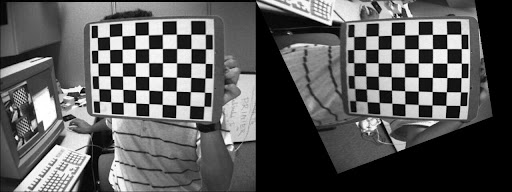
\includegraphics[width=0.8\linewidth]{figures/homography/chessboard_marker.jpg}}
    \caption[Chessboard marker]{An example of a chessboard marker present in a scene that may be used to establish a point correspondence that would serve for a homography transformation. The rectified, fronto-parallel view demonstrates the desired effect that points present on the ``ground'' plane are properly projected, whereas other points suffer from substantial distortion. \externalsrc{\cite{webhomographybasiccode}}}
    \label{fig:ChessboardMarker}
\end{figure}
% ------------------------------------------------------------------------------

% ------------------------------------------------------------------------------
\begin{figure}[t]
    \centerline{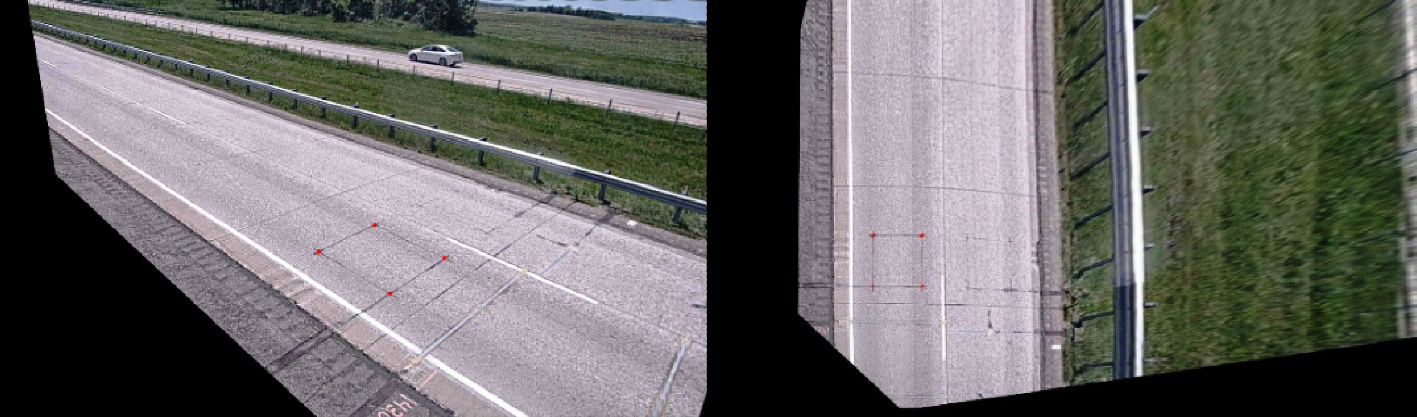
\includegraphics[width=\linewidth]{figures/homography/homography_road.png}}
    \caption[Square marker on a road]{An example of a virtual square marker present on a road that may be used to establish a point correspondence, and thus the homography transformation, too. The obtained view allows for many applications such as speed and size measurements that would otherwise be a lot more problematic in a perspectively deformed view. \externalsrc{\cite{bose2004groundplane}}}
    \label{fig:RoadMarker}
\end{figure}
% ------------------------------------------------------------------------------

A common approach to estimate the homography is to use a set of at least four $2$D point correspondences~\cite{hartley1997defense}. The points that are used for establishing the $2$D point correspondences will be referred to as keypoints. These keypoints may belong to a marker which is an object with a known shape that is either naturally occurring or artificially positioned in the scene. A regular, easy-to-detect pattern (\egtext{}, a chessboard) is commonly utilized~\cite{zhang2016flexible} (\figtext{}~\ref{fig:ChessboardMarker}). A single marker is identified in the image by multiple independent keypoints that have a direct correspondence to its real shape, thus making a group of point correspondences. For the sake of traffic analysis, the marker may be represented by virtually any points on the image as long as certain conditions are met (\figtext{}~\ref{fig:RoadMarker}). However, the point correspondences established this way are often subjected to noise, thus errors may be introduced in the homography estimation. Although $4$ keypoints are satisfactory, often a greater number of keypoints is used, allowing to use optimization to minimize a suitable cost function~\cite{osuna2016multiobjective, mou2013robust}. Subsequently, an outlier removal becomes an important step in the processing pipeline, for which effective and robust algorithms such as RANSAC~\cite{fischler1981ransac} are usually employed.

% ------------------------------------------------------------------------------
\begin{figure}[t]
    \centerline{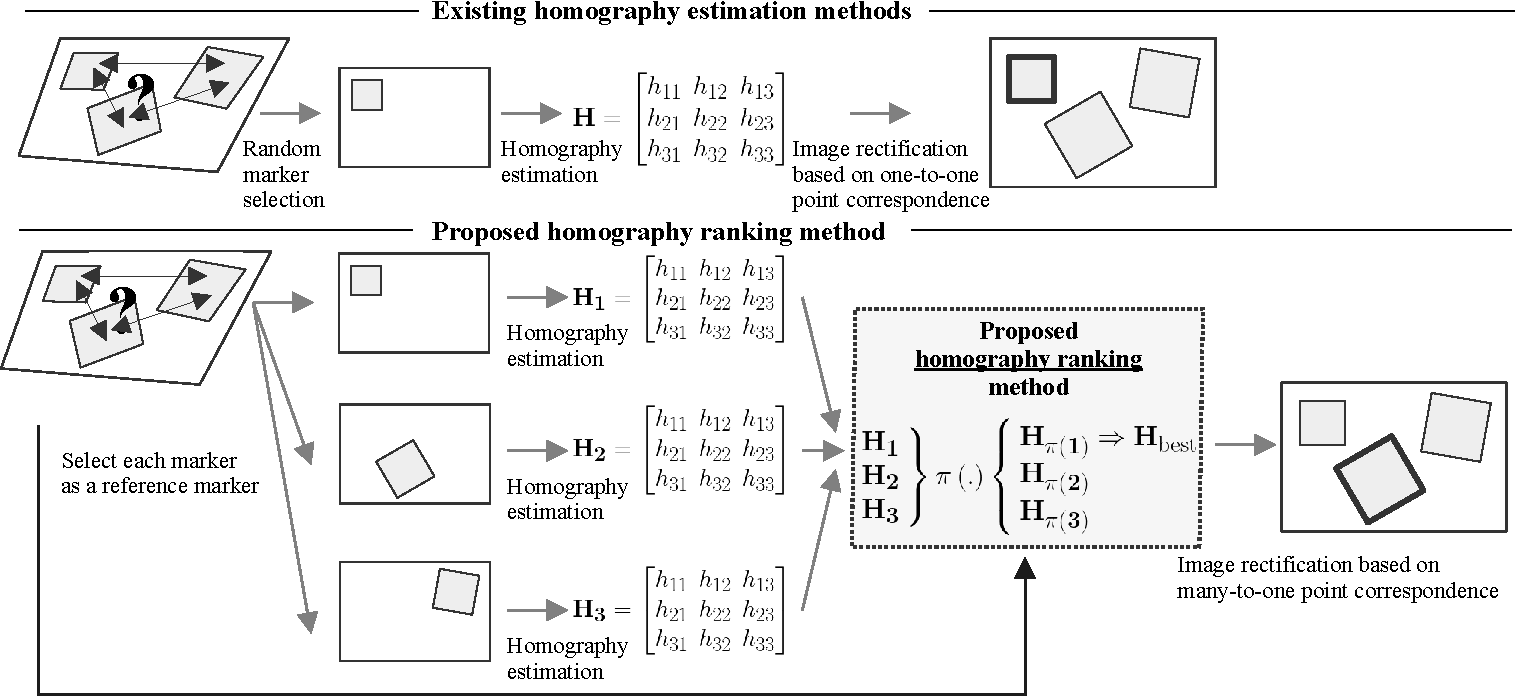
\includegraphics[width=\linewidth]{figures/homography/motivation_diagram.pdf}}
    \caption[Homography ranking motivation diagram]{A fundamental difference between existing homography estimation methods and our proposed method for homography ranking. If there are multiple markers while the information about their relative positions in the world is absent, the existing approaches can only estimate isolated homographies without the ability to select the best one. To address this issue, our method easily serves as an extension to existing approaches by exploiting multiple markers to rank the isolated homographies from the ``best'' to the ``worst''.}
    \label{fig:HomographyMotivationDiagram}
\end{figure}
% ------------------------------------------------------------------------------

A real-world application of generating a bird's-eye view over a road from a video recording when we could not use a large marker to cover a sufficient portion of the road (\figtext{}~\ref{fig:MultipleMarkersOnRoad}) motivated this entire project. We observed that, under our conditions, the homography estimation based on a single small marker was inaccurate. Therefore, there was an attempt to utilize multiple small markers and measure their relative positions. However, as is often the case in practice, their position measurements were highly noisy at best. Thus, we had to bypass the position measurements altogether, which led us to adopt the proposed method, instead. It is crucial to emphasize that our method can also be adopted in a situation when the marker placed at various positions on the same planar surface can be seen at different frames using a static camera. Stacking the captured frames onto each other would effectively yield an artificially generated view of multiple markers.

Assume a presence of a sole marker in the scene (\figtext{}~\ref{fig:RoadMarker}). Moreover, assume the view of the marker is perspectively distorted. If we know its real shape, then it is possible to compute the homography. However, when multiple copies of the same marker are visible, but their positions in the world are unknown, the detailed information about the shape is not enough to incorporate all the keypoints in the estimation. In the absence of position information, existing approaches for homography estimation based on point correspondences do not work because the projection has to preserve the proportional positions. As a result, estimating the homography while not knowing the ground-truth layout of the keypoints up to an arbitrary scale does not guarantee, and often does not even lead, to the correct result.

Under the constraints discussed above, the existing methods can only generate an isolated homography for each marker based on the one-to-one point correspondence (\figtext{}~\ref{fig:HomographyMotivationDiagram}). Each homography may be affected by different sources of noise, \egtext{}, low resolution, blur, or keypoint detection. Thus, the outcome of rectification may vary up to a great extent. In addition, many practical applications often use a marker that just covers a small portion of the image, increasing susceptibility to noise as a result. The trivial solution would be to use a bigger marker that covers the majority of the estimated plane's area. But such a solution is often cumbersome. It is simply not possible to ``merge'' multiple isolated homographies together.

% ------------------------------------------------------------------------------
\begin{figure}[t]
    \centerline{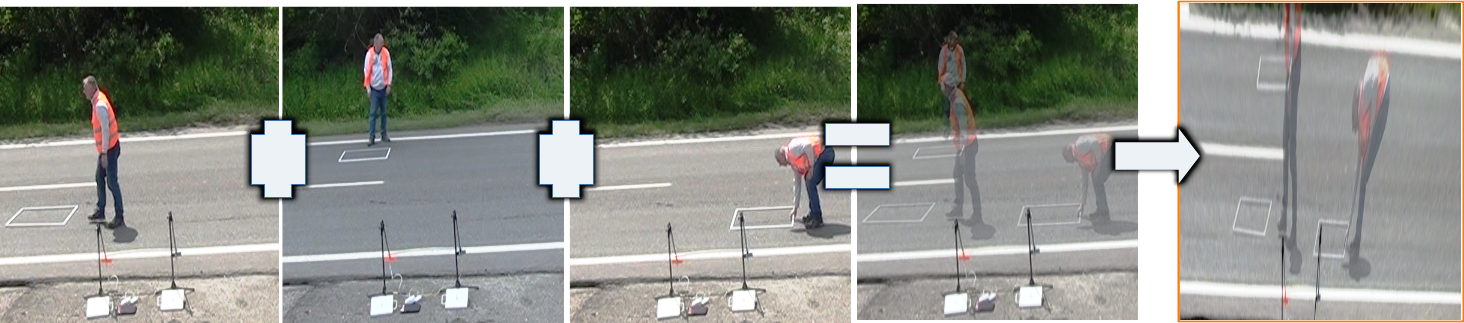
\includegraphics[width=\linewidth]{figures/homography/markers_on_the_road.png}}
    \caption[Multiple markers on the road]{A motivating real-world example. We can see different frames captured during a video recording that show various positions of the same marker. The picture after the ``equality'' sign is a merge of the previous frames for better illustration. Due to the use of a static camera, we may treat the positions of the given marker on individual frames as if they were captured simultaneously. However, the question remains unanswered. Given multiple markers in the absence of their position information, which one is the best to choose for rectification?}
    \label{fig:MultipleMarkersOnRoad}
\end{figure}
% ------------------------------------------------------------------------------
\chapter{Dissertation Thesis Goals}
\label{chap:Goals}

% ========================================
\Gls{vot} is increasingly studied in recent years due to its real-world applications. Given the elaboration provided in chapter \ref{chap:TheoreticalFoundations}, we believe that investing research and development time into the topic of object tracking is worthwhile. The results presented so far are by no means everything that could be said about this topic. Quite to the contrary, the research area is vast, very active, and encompasses a broad range of approaches. Deep learning has occupied a great deal of the time that we spent studying and researching. The intention to build a working solution and incrementally advance the domain of object tracking has been the main incentive behind the choice for the topic of this dissertation thesis. With this in mind, \textbf{the general goal of this dissertation thesis is to improve the accuracy of visual object tracking using deep machine learning tools}.

Tracking of objects using visual features may produce the output in many forms, the usual axis-aligned \glspl{bbox}, rotated \glspl{bbox}~\cite{chen2019rotbboxes}, segmentation masks~\cite{wang2019siammask}, or even object contours~\cite{yang2016encoderdecoder}. We plan to primarily focus on solutions producing axis-aligned \glspl{bbox}. Another variation is the speed at which the tracker processes the input. We have mentioned several times our intention to deal with traffic-related scenarios. So far, there have been no restrictions as to why our tracker would have to run at real-time speed. Many of our real-world applications have involved camera recorded videos that were processed offline. The decision to deal with traffic-related scenarios is also driven by projects supported by the University of Žilina. Companies of the private or public sector are interested in the automated analysis of traffic. Currently, a great deal of work such as vehicle counting is performed with human intervention. The author of this thesis as well as one of the supervisors are actively involved in solving problems related to tracking and traffic analysis using recorded videos.

There are diverse factors that contribute to the overall performance of a tracker. Our analysis has led us to narrow our focus to occlusion handling. Occlusion can impose a huge precision penalty since the tracked object may be lost, or worse, the tracker's attention may be dragged away to a different object. Current \gls{sota} solutions lack explicit occlusion handling~\cite{guo2019siamcar, li2018siamrpn, wang2019siammask} and we have identified this to be one of the leading causes of failure. Thus, \textbf{the specific goal is to propose a solution to problems regarding visual tracking that stem from the presence of occlusion, the transformation of the tracked objects as well as varying lighting conditions in the scene}.

Given what has been presented so far, we have chosen the path of similarity learning and \gls{reid} (section \ref{ssec:LearningMetricEmbedding}). Despite the existence of different techniques, we have been convinced during this initial research phase about the great potential of metric spaces and their properties that seem to fit our needs~\cite{liu2016ssd}. Our research of modern publications brought forward in the previous chapters points to the direction of embeddings and metric learning (section \ref{sec:LatentSpacesAndEmbeddings}), specifically when applied to \gls{reid}. Besides the possibility to employ motion models for better prediction of locations in the absence of visual input, some research papers indicate that a well-built similarity function based upon metric learning in combination with a simple matching algorithm on the level of \glspl{bbox} can produce a reasonable performance~\cite{tao2016sint}. We think that even humans would be capable of discerning between objects when shown their pictures from distinct times in a video even dozens of seconds apart. The inherent visual clue about the object that makes it stand out among the set of others should be present most of the time. Variation in lightning should not dramatically influence the outcome. However, it may not be always possible to unambiguously identify an object given its appearance, especially when it comes to vehicles. Special marks such as customized paintings, decorations, or even scratches become relevant~\cite{liu2016ssd}. In those situations, it is crucial to exploit temporal information. Expanding upon the foundation of the specific goal, we will strive to propose and implement a solution that can improve the performance of a tracker by considering the obstacles mentioned above. Therefore, \textbf{the goal from a methodological perspective is the application of approaches based on \gls{reid} and similarity learning to support the solution to problems caused by the object occlusion of varying intensity, change in the position, and the viewpoint of the tracked object, and fluctuations in the scene illumination}.

In order to accomplish the aforementioned goals, this dissertation thesis should follow the steps given below:
\begin{itemize}
    \item Identification of major problems that occur in the task of visual object tracking.
    \item Outline of requirements for datasets for training and evaluation of models along with a possibility of comparison with other approaches.
    \item Adequate data preprocessing, either as a modification of existing datasets or creating new ones for object tracking, particularly in traffic-related scenarios.
    \item Analysis of the current \gls{sota} approaches dealing with visual tracking of objects.
    \item Review of the modern methods of \gls{reid} based on similarity learning. Assessment of the contrastive-based and triplet-based training paradigms.
    \item The exploitation of recent advances in object \gls{reid} to handle object occlusion and dynamic conditions in terms of illuminance and object position. 
    \item Design and implementation of a method for visual object tracking adopting advances in deep machine learning.
    \item Evaluation of the implemented method with respect to official benchmarks.
    \item Summarization and dissemination of the achieved results followed by recommendations for their practical applications.
\end{itemize}

\chapter{Theoretical Foundations}
\label{chap:TheoreticalFoundations}

\section{Neural Networks}

In this short section, we briefly describe artificial neural networks and their various types relevant to this thesis. However, our assumption is that the reader is sufficiently equipped with the knowledge regarding deep machine learning, and thus, for the sake of keeping this document as short as possible, we will omit detailed elaboration.

% ##############################################################################
\subsection{Artificial Neural Networks}
\label{ssec:ArtificialNeuralNetworks}

Artificial neural networks (or just neural networks for short) are computing systems that are inspired by, but not identical to, biological neural networks that constitute animal brains. Such systems essentially \emph{learn} to perform tasks by considering multiple samples, generally without being programmed with task-specific rules. Within recent decades, under the influence of constantly growing computational power and our data collecting and data processing capabilities, this technology has acquired a status of paramount importance when solving a problem using machine learning. They are a quintessential deep learning model. Artificial neural networks are also known in the literature as the multilayer perceptron~\cite{rosenblatt1958perceptron}, feedforward neural networks or deep feedforward neural networks~\cite{goodfellow2016dl}.

In mathematical terms, the goal of a neural network is to approximate some unknown function $f$. For instance, when considering a classifier, the transformation $y = \func{f}{\vx}$  maps the given input $\vx$ to a category $y$. Such a network, therefore, defines a mapping and learns the value of the parameters that result in the best function approximation~\cite{goodfellow2016dl}.

The name \emph{feedforward} is derived from the fact that the information flows through the function being evaluated from $\vx$, through the intermediate computations, and finally to the output $\vy$. Moreover, the feedforward neural networks are called networks since they are typically represented as a composition of multiple different functions. Such a model can be described with a directed acyclic graph denoting the sequential composition of several functions. More concretely, we might have three functions $\suprbrackets{f}{1}$, $\suprbrackets{f}{2}$ and $\suprbrackets{f}{3}$, forming a chain, $\func{f}{\vx} = \func{\suprbrackets{f}{3}}{\func{\suprbrackets{f}{2}}{\func{\suprbrackets{f}{1}}{\vx}}}$. These chain structures are the most commonly used structures in neural network models~\cite{goodfellow2016dl} (see \figtext{}~\ref{fig:WebFCArchitecture}). Deep machine learning consists of multiple such layers of neurons stacked onto each other that are trained using the \emph{backpropagation} algorithm~\cite{rumelhart1986backprop}. Our work will rely heavily upon the aforementioned deep neural networks, especially convolutional neural networks, discussed next.

% ------------------------------------------------------------------------------
\begin{figure}[t]
    \centerline{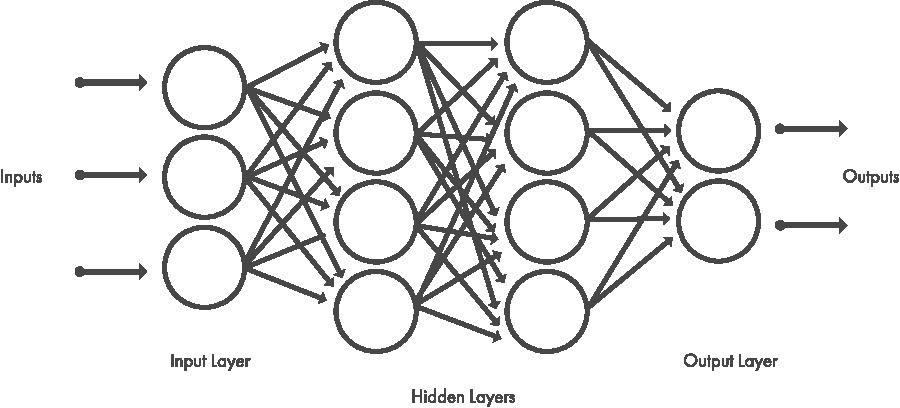
\includegraphics[width=0.7\linewidth]{figures/theoretical_foundations/typical_fcn_architecture.pdf}}
    \caption[A typical FC architecture]{An illustration of a typical fully connected neural network. \externalsrc{\cite{webfcarchitecture}}}
    \label{fig:WebFCArchitecture}
\end{figure}
% ------------------------------------------------------------------------------

% ##############################################################################
\subsection{Convolutional Neural Networks}
\label{ssec:ConvolutionalNeuralNetworks}

This type of neural networks has gained popularity in the computer vision community thanks to a never-seen-before performance on image classification task~\cite{krizhevsky2012classification}. This machine learning algorithm processes images or other high dimensional, grid-like input and then learns the importance (weights and biases) of various aspects of the input data. Even though \glspl{cnn} can handle $1D$ time series data and be a counterpart to \glspl{rnn}~\cite{franoischollet2017learning}, our primary focus is to process $3D$ tensors. Simply put, convolutional networks are artificial neural networks that use in at least one of their layers the convolution operation instead of a general matrix multiplication~\cite{goodfellow2016dl} (see \figtext{}~\ref{fig:WebCNNArchitecture}).

The successful ability of these networks to capture spatial and temporal properties via learned convolutional filters is the fundamental principle. Let $f$ and $g$ be functions. Then, the operation of convolution denoted by $\star$ produces a third function, as a result of the following computation (demonstrating the commutativity property, too)~\cite{goodfellow2016dl}:
\begin{equation}
    \label{eq:ConvolutionContinuous}
    \func{\rbrackets{f \star g}}{t} =
    \int_{-\infty}^{\infty}
    \func{f}{\tau}
    \func{g}{t - \tau}
    d\tau =
    \int_{-\infty}^{\infty}
    \func{f}{t -\tau}
    \func{g}{\tau}
    d\tau.
\end{equation}
In this setting, $f$ is be the input, and $g$ is the kernel. The output of this operation is a feature map. During the training, the aim is to learn the weights of the kernel matrix (similar to general artificial neural networks) that produces a feature map based on which the model can solve the given task according to some objective function.

Let $I$ be a two-dimensional input image and $K$ be a two-dimensional kernel. Then, for a given position $\rbrackets{i, j}$ in the input image $I$, the convolution can be written in its discrete form as
\begin{equation}
    \label{eq:ConvolutionDiscrete}
    \func{\rbrackets{f \star g}}{i, j} =
    \sum_{m}
    \sum_{n}
    \func{I}{m, n}
    \func{K}{i - m, j - n}.
\end{equation}
Nonetheless, many machine learning libraries implement the cross-correlation operation, not the convolution operation by its strict definition. This operation is the same except for the fact that the kernel is not flipped, thus the commutative property is not preserved, which is not demanded in neural networks. In that case, the result of the cross-correlation is given by~\cite{goodfellow2016dl}

\begin{equation}
    \label{eq:CrossCorrelation}
    \func{\rbrackets{f \star g}}{i, j} =
    \sum_{m}
    \sum_{n}
    \func{I}{i + m, j + n}
    \func{K}{m, n}.
\end{equation}

An indispensable outcome of \glspl{cnn} is the ability to capture hierarchical relations. Layers placed near the input of the model capture low-level features such as edges, colors, gradient orientations, and so on. On the other hand, layers placed further, deeper in the model, highlight semantic, abstract features that are specific to the task at hand. We will refer to this fact many times in our work since visual object trackers need to accurately discriminate between the foreground and background as well as properly generalize. The exploitation of the mentioned qualities of convolutional layers will be demonstrated in \sectiontext{}~\ref{sec:VisualObjectTracking}.

Another prominent use case of \glspl{cnn} is \emph{transfer learning}, where a pretrained model is adopted for a new task, utilizing the already learned features. These pretrained models may come in various flavors, but typical ones are pretrained for an image classification task using the \datasetname{ImageNet} dataset~\cite{deng2009imagenet}. The reasoning is that visual features such as edges and contours are vital to general object recognition tasks, hence it is not needed to learn coarse, rudimentary, low-level features from scratch all the time. Our work will certainly require the \emph{transfer learning}, and also additional \emph{fine-tuning} of the pretrained model of choice.

% ------------------------------------------------------------------------------
\begin{figure}[t]
    \centerline{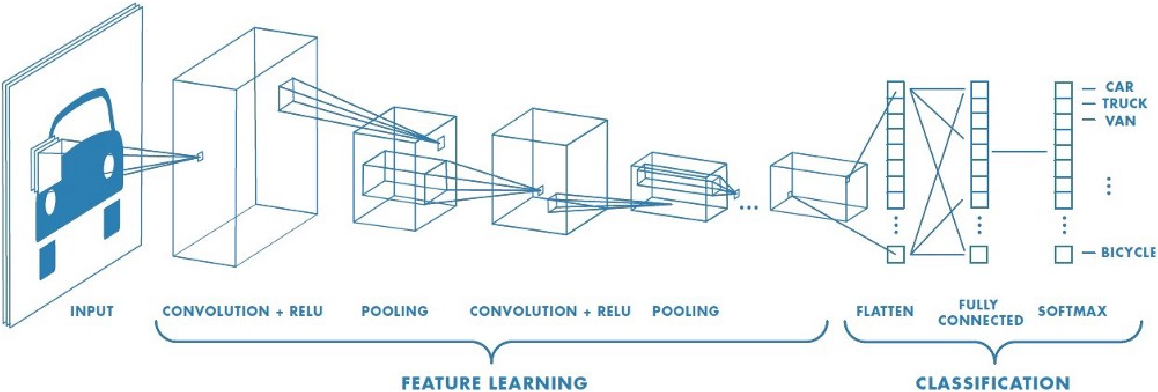
\includegraphics[width=0.9\linewidth]{figures/theoretical_foundations/typical_cnn_architecture.pdf}}
    \caption[A typical CNN architecture]{An illustration of a typical convolutional neural network architecture for a quintessential classification task. An image of a car is fed into the model that extracts visual features that are subsequently processed by the fully connected layers resulting in the probability distribution over target classes. \externalsrc{\cite{webcnnarchitecture}}}
    \label{fig:WebCNNArchitecture}
\end{figure}
% ------------------------------------------------------------------------------

\section{Object Detection}
\label{sec:ObjectDetection}

Since the topic of this thesis concerns the task of \emph{visual} object tracking, an indispensable step in the processing pipeline will unquestionably be object detection. Here we give an overview of various types of image inference to highlight the importance of object detection. The general task of image inference comes in three types, where each builds upon the previous one. The dependency chain is the following: \emph{object classification} $\to$ \emph{object detection} $\to$ \emph{image segmentation}. Due to length constraints for this document, we will focus on object detection as it is the most important of the three for \gls{vot}. We do admit that the object detection strongly relies upon classification because the object cannot be localized (bound) without classifying it.

Object detection comes in various types discussed in the following sections. For our purposes, we will focus on applying the current \gls{sota} techniques with no intention of significantly contributing to object detection methods themselves. Nevertheless, we will put a great emphasis on the performance of the chosen algorithm, since faulty detection with high confidence can hardly be corrected later on. From a holistic point of view, there are \emph{fast} object detectors, such as the most prominent one, \gls{yolo}~\cite{Redmon2016} (section~\ref{ssec:YouLookOnlyOnce}), or \gls{ssd}~\cite{Liu2016}. Here we use the term \emph{fast} to denote that the detector can operate on high \gls{fps}. This comes at a cost of relatively lower accuracy, though, as compared to \emph{slower} but more accurate approaches based on region proposals, such as various versions of \glspl{rcnn} (section \ref{ssec:FasterRCNN}).

Historically speaking, object detection in its early stages of development depended on feature engineering followed by some shallow machine learning model (e.g. \gls{svm}~\cite{cortes1995support}) to classify the proposed object. Feature extraction was achieved using approaches such as \gls{sift}~\cite{Lowe1999}, an algorithm capable of producing description of local features in images. Another eminent approach was \gls{hog}~\cite{osti_6007283}, equally used for feature extraction by taking advantage of a change in orientation of gradients in localized portions of the image and subsequently counting occurrences of various orientations. But, as we stated, robust object detection is what our task demands, and the goal of getting the top performance is unattainable without deep learning-based object detection, the principal topic of this section.

Object detection is by its very nature a difficult task, because the number of objects is unknown in advance, which means, that the number of outputs of the model is variable. In terms of a standard deep learning model as described in section~\ref{ssec:ArtificialNeuralNetworks}, this represents a nuisance. A plethora of attempts have been proposed to evade this inherent shortage of standard neural networks. An obvious solution is to only produce a constant number of \glspl{bbox}, as utilized by \gls{ssd} and \gls{yolo}, for instance. But methods based on region proposals try to circumvent the obstacle of having to predict only a fixed set of \glspl{bbox}. Other differences between object detectors stem from the architecture itself, whether the training is an end-to-end pipeline or the model consists of various parts. Fully convolutional architectures are also becoming more prevalent and the latest results are promising~\cite{Tian2019}. We will also review fully convolutional trackers in great detail in section \ref{ssec:FullyConvolutionalTracking}.

% ##################################################
\subsection{Non-Maximum Suppression}
\label{ssec:NonMaximumSuppression}

Before we dive into the description of the detection itself, we first introduce a general post-processing approach for test phase inference of an object detector. A typical object detection pipeline employs a region proposal step for object classification. Object detectors have hugely profited from the so-called end-to-end learning paradigm in which proposals, features, and the classifier become part of one neural network model~\cite{Hosang2017}. A proposal, in this setting, is nothing but a region containing a potential object of interest. However, the number of proposals may grow considerably, outnumbering the real count of present objects of interest. Moreover, these proposals may have a large overlapping region as measured by \gls{iou} (section \ref{eq:IntersectionOverUnion}), rendering most of them useless in terms of conveying new information, as the majority could cover pretty much the same region. To filter such proposals and extract only the relevant ones, the \gls{nms} algorithm introduced below is used (see Fig.~\ref{fig:NonMaximumSuppression}). This post-processing algorithm is responsible for uniting all detected \glspl{bbox} belonging to the same object~\cite{Hosang2017}.

The central idea is to iteratively select only region proposals the \gls{iou} of which is below a specific threshold, i.e. the area they share does not exceed a particular value. But the search for proposals is executed with respect to their confidence level (detection score), since regions produced with higher score should be preserved first. Another reason to evade the occurrence of false positives with high confidence during the detection as much as possible.

For a more formal description, let $\mset{B} = \cbrackets{\vect{b}_1, \vect{b}_2, \dots, \vect{b}_n}$ be a set of $n$ region proposals described by $n$ \glspl{bbox}. Scores for each detection are contained in a set $\mset{S} = \cbrackets{s_1, s_2, \dots, s_n}$, where $s_i$ denotes a detection score for the $i$-th box, $\vect{b_i}$. Let $\lambda$, such that $0 \leq \lambda < 1$, denote a threshold for the maximum allowed portion of the overlap between regions. $\mset{B}_{nms}$ is the set of filtered proposal instances from the set $\mset{B}$ produced using the \gls{nms} algorithm below (inspired by~\cite{Bodla2017}):

\begin{algorithmic}[1]
    \Function{NMS}{$\mset{B}$, $\mset{S}$, $\lambda$}
    
        \State $\mset{B}_{nms}$ $\gets$ $\emptyset$
        \Comment{initialize the output (filtered) set of region proposals}
        
        \While {$\mset{B} \neq \emptyset$}
            \Comment{loop until all the proposals are processed}
            
            \State $m \gets \underset{i \in \cbrackets{1, 2, \dots, \msetsize{S}}}{\argmax{}} \mset{S}$
            \Comment{find an index of a proposal with the highest score}
            
            \State $\mset{B} \gets \mset{B} - \vect{b}_m$, $\mset{S} \gets \mset{S} - s_m$
            \Comment{remove the proposal}
            
            \State $\mset{B}_{nms} \gets \mset{B}_{nms} \cup \vect{b_m}$
            \Comment{save the proposal with the highest score}
            
            \For{$i \gets 1$ to $\msetsize{B}$}
            \Comment{iterate through remaining proposals}
            
                \If{\Call{iou}{$\vect{b}_m$, $\vect{b}_i$} $\geq \lambda$}
                \Comment{\gls{iou} (equation~\ref{eq:IntersectionOverUnion}) exceeds the threshold}
                
                    \State $\mset{B} \gets \mset{B} - \vect{b}_i$, $\mset{S} \gets \mset{S} - s_i$
                    \Comment{remove the proposal}
                \EndIf
            \EndFor
        \EndWhile
        
        \State \Return $\mset{B}_{nms}$
    \EndFunction
\end{algorithmic}

\begin{figure}[t]
    \centerline{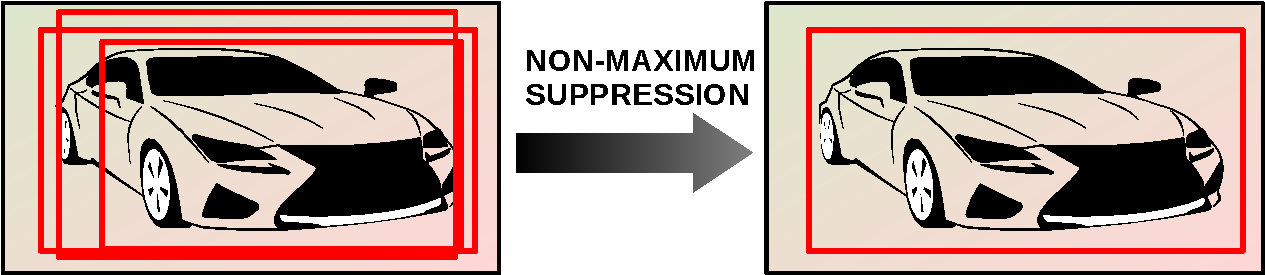
\includegraphics[width=0.7\linewidth]{figures/theoretical_foundations/non_maximum_suppression.pdf}}
    \caption[\Gls{nms} visualization]{An illustration of a potential effect of the \gls{nms} algorithm on \glspl{bbox}. Multiple proposals (left) are filtered so that only the ones with the highest detection score (right) remain while satisfying the condition that the overlap does not exceed a specific threshold.}
    \label{fig:NonMaximumSuppression}
\end{figure}

% ##################################################
\subsection{YOLO}
\label{ssec:YouLookOnlyOnce}

\Gls{yolo} is a very popular object detector thanks to its ability to run in real-time and yet be very accurate. Its speed is primarily a consequence that \emph{it looks only once} at a given input image. Compared to region proposal-based approaches, where each object proposal has to be classified separately, resulting in multiple inferences by a potentially huge neural network model, the authors of \gls{yolo} devised a \gls{cnn} model capable of performing extraction of region proposals as well as classification in a single run~\cite{Redmon2016}. Besides, the backbone \gls{cnn} model responsible for handling the visual input processes an entire image during the training and test time, allowing the implicit inclusion of contextual information about classes together with their visual representation. During the testing phase, after the single forward propagation through the neural network is executed, the \gls{nms} algorithm is employed to filter predictions to make sure that each object instance is detected just once. It is needless to say that \Gls{yolo} performs well at learning representations that make the generalization easier, which makes this approach well suited for a general object detector, as long as it has been trained on the target domain~\cite{Redmon2016}. Since the initial introduction of this approach~\cite{Redmon2016}, multiple updates have been brought forward, either from the main author himself~\cite{Redmon2017, Redmon2018}, or from other researchers~\cite{Wang, Wong2019}. Such an interest supports the assertion that \gls{yolo} has great potential for further research as well as real-world applications. In our work, it is a prominent candidate for an object detector that we would train specifically for detecting vehicles and become a part of the object tracking pipeline.

The main implementation aspect is the unification of separate components of object detection into a single neural network. Training is thus executed in an end-to-end fashion. In the original article~\cite{Redmon2016}, the model was pre-trained on ImageNet~\cite{imagenet_cvpr09} classification task at half the resolution of $224 \times 224$. When detecting, the resolution was doubled to get required $448 \times 448$ (Fig.~\ref{fig:YOLOGeneralIdea}). The network uses features from the entire image for the prediction of each \gls{bbox}. It also simultaneously predicts all \glspl{bbox} across all classes~\cite{Redmon2016}.

As shown in Fig.~\ref{fig:YOLOBBOXESProgression}, the input image is divided into an $S \times S$ grid. Since most of the time an object will overlap multiple grid cells, the \emph{main} cell responsible for predicting the object will be the one the center of the object's \gls{bbox} falls into. Each \gls{bbox} prediction is evaluated by a confidence level computed as $\prob{\text{object}} \cdot \func{IOU}{\vect{b}_{pred}, \vect{b}_{truth}}$, with $\vect{b}_{pred}$ and $\vect{b}_{truth}$ being the prediction and ground truth, respectively. If no object exists in a particular cell, the confidence should be equal to $0$. Each grid cell prediction also encapsulates $C$ conditional probabilities for each class under the assumption that the object is present, mathematically stated as $\probgiven{{\text{class}}_i}{\text{object}}$. But only one set of class probabilities is predicted per grid cell, regardless of the value of the hyperparameter $B$. This description can be concisely conveyed by the equation below:
\begin{equation}
    \begin{aligned}
        \label{eq:YOLOCOnfidenceScores}
        &\probgiven{{\text{class}}_i}{\text{object}}
        \cdot
        \prob{\text{object}}
        \cdot
        \func{IOU}{\vect{b}_{pred}, \vect{b}_{truth}}
        =\\
        &\prob{{\text{class}}_i}
        \cdot
        \func{IOU}{\vect{b}_{pred}, \vect{b}_{truth}}.
    \end{aligned}
\end{equation}
This equality gives the class-specific confidence score which basically encodes both the probability of the $i$-th class appearing in a particular \gls{bbox} in conjunction with how well this predicted box fits the object.

\begin{figure}[t]
    \centerline{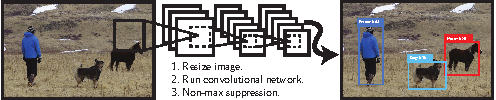
\includegraphics[width=0.8\linewidth]{figures/theoretical_foundations/yolo_general_idea.pdf}}
    \caption[\Gls{yolo} processing pipeline]{Processing of images using \gls{yolo} requires the input image to have the resolution of $448 \times 448$ pixels. Then, a single run of the convolutional network happens, followed by the thresholding of the resulting detections according to their confidence. \externalsrc{\cite{Redmon2016}}}
    \label{fig:YOLOGeneralIdea}
\end{figure}

\begin{figure}[t]
    \centerline{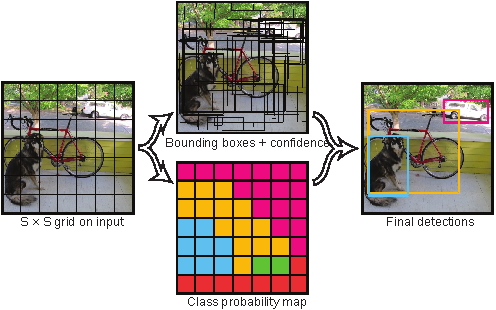
\includegraphics[width=0.8\linewidth]{figures/theoretical_foundations/yolo_bboxes_progression.pdf}}
    \caption[\Gls{yolo} detections]{This model treats detections as a regression problem. The image is divided into $S \times S$ grids, for each grid $B$ \glspl{bbox} are predicted with associated confidence, and for each box $C$ class probabilities are inferred. The prediction tensor has therefore size of $S^2 \times \rbrackets{5B + C}$. \externalsrc{\cite{Redmon2016}}}
    \label{fig:YOLOBBOXESProgression}
\end{figure}

The network design reflects a standard practice in deep learning-based computer vision model, where a \gls{cnn} backbone is used to extract features followed by fully connected layers. In this case, the two fully connected layers are in charge of prediction of the output probabilities and coordinates (Fig.~\ref{fig:YOLOArchitecture}).

\begin{figure}[t]
    \centerline{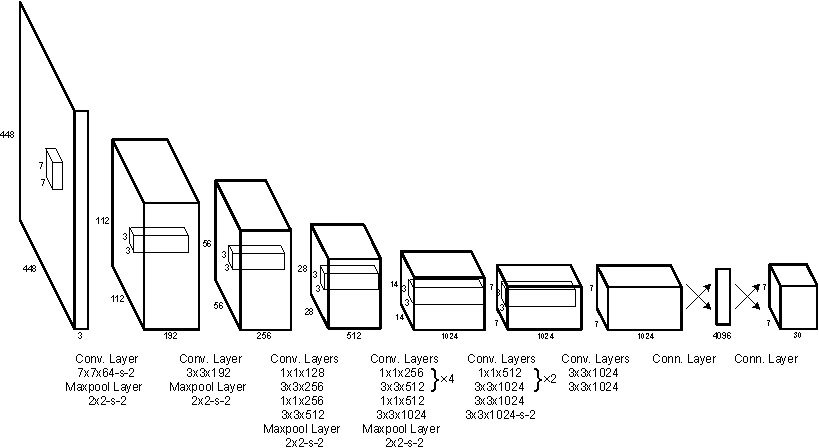
\includegraphics[width=0.8\linewidth]{figures/theoretical_foundations/yolo_architecture.pdf}}
    \caption[\Gls{yolo} architecture]{The \gls{yolo} model architecture consisting of 24 convoutional layers followed by two fully connected layers at the end. The alternation of $1 \times 1$ convolutional layers is used to reduce the feature space size. \externalsrc{\cite{Redmon2016}}}
    \label{fig:YOLOArchitecture}
\end{figure}

% ##################################################
\subsection{Faster R-CNN}
\label{ssec:FasterRCNN}

Apart from the two already introduced approaches, this one, \modelname{Faster R-CNN}, employs \emph{two-stage} object detection. The first stage consists of generating region proposals using the \gls{rpn}~\cite{Ren2017} (Fig.~\ref{fig:FasterRCNNRPN}), where the input image is processed by a feature extractor~\cite{Huang2017}. These class-agnostic proposals, a set of rectangular boxes, are produced from an input of arbitrary size (allowed by the fact that this process is modeled by a fully convolutional network) (Fig.~\ref{fig:FasterRCNNMetaArch}).

As far as the second stage is concerned, the proposed regions (usually $300$) serve as a basis for subsequent cropping of features from the same intermediate feature map which are then fed to the remaining feature extractor to predict the class. Based on this class prediction, the proposed box is further refined. The name for this stage is \emph{box classifier}.

\begin{figure}[t]
    \centerline{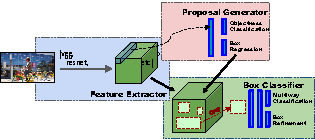
\includegraphics[width=0.7\linewidth]{figures/theoretical_foundations/faster_rcnn_metaarchitecture.pdf}}
    \caption[\modelname{Faster R-CNN} meta-architecture]{A meta-architecture of the \modelname{Faster R-CNN} model. \externalsrc{\cite{Huang2017}}}
    \label{fig:FasterRCNNMetaArch}
\end{figure}

As the endeavor is to diminish unnecessary computations, the proposals are not cropped explicitly from the input image, and then processed by the feature extractor. Nevertheless, there is a part of the computation that has to be executed once per each proposed region, so the performance depends on the number of regions generated by the \gls{rpn}.

\begin{figure}[t]
    \centerline{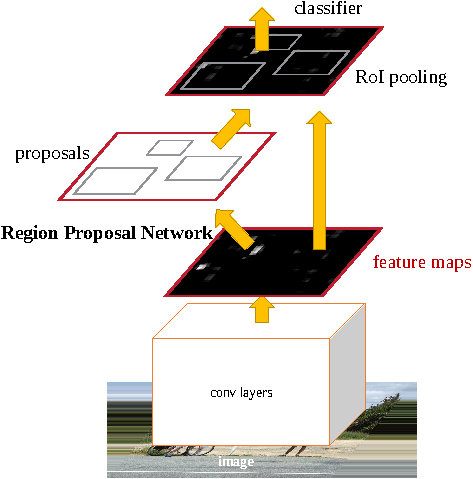
\includegraphics[width=0.5\linewidth]{figures/theoretical_foundations/faster_rcnn_rpn_module.pdf}}
    \caption[\modelname{Faster R-CNN} with the \gls{rpn}]{The \modelname{Faster R-CNN} is built as a unified network for object detection, with its \gls{rpn} module serving the purpose of an \emph{attention}. \externalsrc{\cite{Ren2017}}}
    \label{fig:FasterRCNNRPN}
\end{figure}

% ##################################################
\subsection{Fully Convolutional Object Detection}
\label{ssec:FullyConvolutionalObjectDetection}

\todo[inline]{Emphasize centerness more since SiamMOT exploited it, too. Also mention Siamese architectures that also used it.}

Recent research shows that utilizing fully convolutional networks provides many advantages. Not only the input can be of arbitrary size thanks to the absence of fully connected layers, but the number of hyperparameters is reduced, too. We will now discuss the \gls{fcos} model. This work was inspired by one-stage detectors such as \gls{yolo} and \gls{ssd} and by how semantic segmentation operates on the level of pixels. The proposed solution by~\cite{Tian2019} is anchor-free as well as proposal-free. The elimination of anchors avoids complicated computations related to anchor boxes, such as calculating overlapping regions during training. More importantly, anchor boxes come with many initialization-sensitive hyperparameters, namely their number and dimensions.

\Gls{fcos} is built on top of \gls{fpn}~\cite{Li2019}, which aggregates features from the backbone at multiple levels, reminiscing a pyramidal shape. Predictions are thereafter obtained across $5$ feature levels from the \gls{fpn} (Fig.~\ref{fig:FCOSFeaturePyramid}). \gls{fpn} makes use of the scale-invariant properties of feature pyramids, which enable object detection over a wide range of scales.

Authors came up with a concept of \emph{centerness}, which describes the amount of deviation of the pixel's location from the object center (Fig.~\ref{fig:FCOSCenterness}). The reason for adding this score was to suppress locations that are further away from the object's center, because they produced low-quality \gls{bbox} predictions. This score is then used as a weighting factor for the class prediction score. Let $l^*$, $t^*$, $r^*$ and $b^*$ be the regression targets for the box. Then the \emph{centerness} $\func{C}{\cdot}$ is computed as

\begin{equation}
    \label{eq:CenternessDetection}
    \func{C}{l^*, t^*, r^*, b^*} =
    \sqrt{
        \frac{
            \func{\min}{l^*, r^*}
        }{
            \func{\max}{l^*, r^*}
        }
        \times
        \frac{
            \func{\min}{t^*, b^*}
        }{
            \func{\max}{t^*, b^*}
        }
    }.
\end{equation}


\begin{figure}[t]
    \centerline{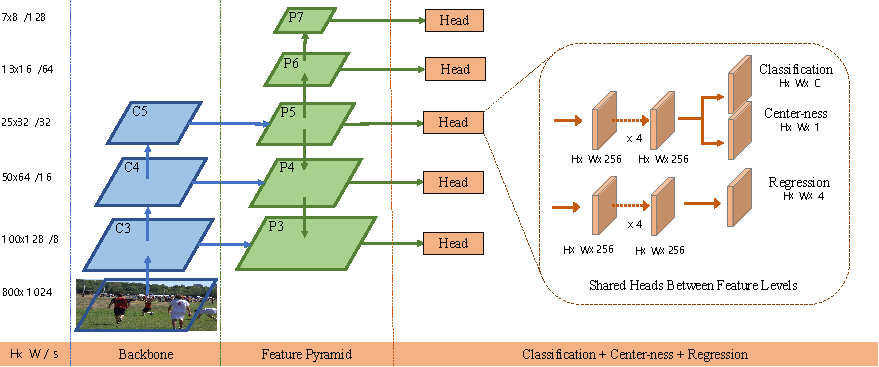
\includegraphics[width=\linewidth]{figures/theoretical_foundations/fcos_feature_pyramid.pdf}}
    \caption[\Gls{fcos} architecture]{The network architecture of the \gls{fcos}. Feature maps denoted by $C3$, $C4$ and $C5$ belong to the backbone network. Features at the levels from $P3$ to $P7$ are used to make final predictions. For each of these feature maps, the shared head computes the classification (foreground/background disrimination), the \emph{centerness} score and \gls{bbox} regression. \externalsrc{\cite{Tian2019}}}
    \label{fig:FCOSFeaturePyramid}
\end{figure}

\begin{figure}[t]
    \centerline{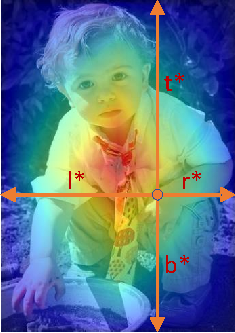
\includegraphics[width=0.25\linewidth]{figures/theoretical_foundations/fcos_centerness.pdf}}
    \caption[Centerness visualization]{Red, blue, and other colors denote $1$, $0$ and the values between them, respectively. Center-ness is calculated as given by eqiation~\ref{eq:CenternessDetection} and decays from $1$ to $0$ as the location deviates from the center of the object. Best viewed in color. \externalsrc{\cite{Tian2019}}}
    \label{fig:FCOSCenterness}
\end{figure}

\begin{figure}[t]
    \centerline{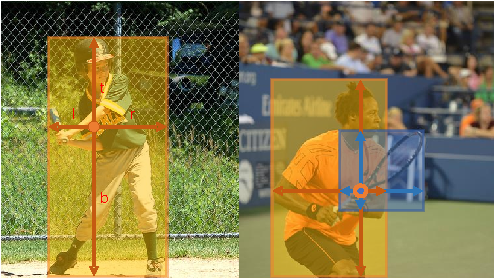
\includegraphics[width=0.6\linewidth]{figures/theoretical_foundations/fcos_detection_demo.pdf}}
    \caption[\Gls{fcos} predictions]{On the left, the model predicts for each pixel in the image a $4D$ vector $\sbrackets{l, t, r, b}^T$ encoding the \gls{bbox} dimensions (supervised by the ground-truth one during the training). On the right, there is a demonstration of possible ambiguity when a pixel resides within more than just one \gls{bbox}. In that case, a decision has to be made which box should be regressed to. \externalsrc{\cite{Tian2019}}}
    \label{fig:FCOSDetectionDemo}
\end{figure}

\section{Latent Spaces and Embeddings}
\label{sec:LatentSpacesAndEmbeddings}

In our work, we will often discuss the use of so-called \emph{embedings} for occlusion handling during the process of \gls{vot}. After an object emerges on a scene, there is an imminent need to assign it to either an existing track or mark the object as a new one. We believe the approach further described has the potential to significantly contribute to occlusion handling, either directly or indirectly. To this end, one idea is to learn a metric embedding.

% ##############################################################################
\subsection{Learning Metric Embedding}
\label{ssec:LearningMetricEmbedding}

As~\cite{hermans2017triplet} describes, the goal of learning metric embedding is to learn a function (a transformation) $\func{f_\theta}{x}: \mathbb{R}^F \to \mathbb{R}^D$, which maps semantically similar points from the data manifold in $\mathbb{R}^F$ onto metrically close points in $\mathbb{R}^D$. Analogously, $\func{f_\theta}{\cdot}$ should map semantically different points in $\mathbb{R}^F$ onto metrically distant points in $\mathbb{R}^D$. Learning such a metric embedding is similar to dimensionality reduction, as it involves mapping a set of high dimensional input points onto a low dimensional manifold. The function $\func{f_\theta}{\cdot}$ ideally maps \emph{similar} (a measure of similarity has to be defined) points in the input space to nearby points on the manifold~\cite{hadsell2006dimreduction}.

To clarify, suppose the use of this transformation for vehicle \gls{reid}. This embedding would be achieved by a learned function that would map the images of vehicles into a latent space, where images of the same vehicle would be mapped closer together. Moreover, such mapping should be invariant to variations in lighting conditions, vehicle rotations (a difficult one can be a change from front to rear view), and many other transformations that interfere with vehicle \gls{reid}. Kuma~\etal{}~\cite{kuma2019vehiclereid} also mention that popular loss functions for learning embeddings include contrastive or triplet loss, the two we discuss further in the section~\ref{ssec:SiameseAndTripletNetworks}. Among other things, embedding trained this way can be used to produce a feature vector for classification, one-shot learning tasks~\cite{koch2015siameseoneshot}, clustering~\cite{schroff2015facenet}, face recognition~\cite{parkhi2015deepface} and last, but not least, re-identification~\cite{kuma2019vehiclereid}.

Embedding, or mapping the input into some latent space with specific properties, is of great use even in combination with \glspl{gan}~\cite{goodfellow2014gans}. A prominent work of researches from webnvidia company~\cite{webnvidia} demonstrates how individual facial features can be modified once the image of the person's face is mapped (embedded) into an adequate latent space~\cite{karras2020stylegan}. Manipulations ranging from a change in hair and skin color through facial expressions (e.g. smile) up to the person's age or gender are possible using just linear vector operations. Briefly, once the user obtains the corresponding vector of the person's face image in the latent space formed during the training phase, then simply adding or subtracting a vector which corresponds to the ``age direction'' results in making the person younger or older. All of this is achieved in a purely linear fashion. Even though such a generator-based architecture is by itself of no use for \gls{reid}, this approach initially led us to consider the exploration of latent spaces. Nonetheless, \glspl{gan} may provide a synthetically generated different views of the same vehicle (rear, front, etc.) to enhance the training on \emph{hard cases}~\cite{lou2019embreid} (further discussed in section \ref{ssec:TripletMiningStrategies}).

% ##############################################################################
\subsection{Siamese and Triplet Networks}
\label{ssec:SiameseAndTripletNetworks}

\begin{figure}[t]
    \centering
    \begin{subfigure}[b]{0.49\textwidth}
        \centering
        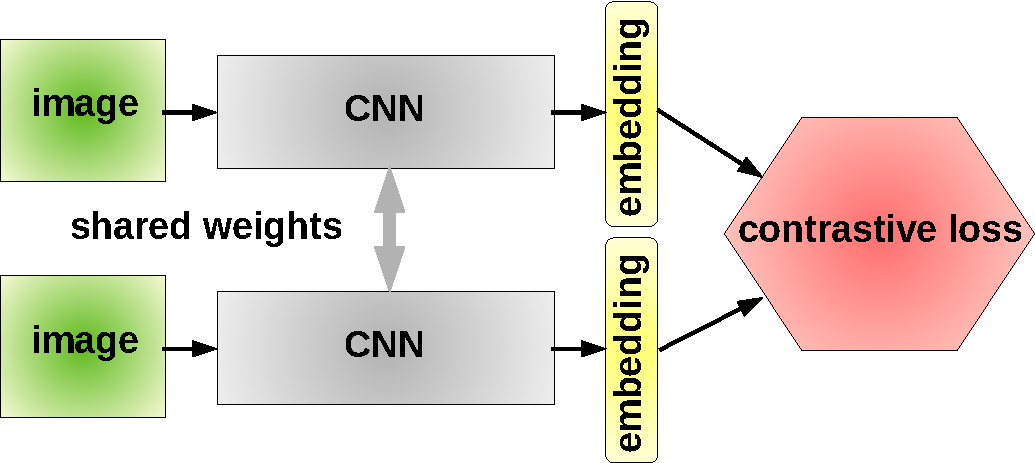
\includegraphics[width=\textwidth]{figures/theoretical_foundations/siamese_architecture.pdf}
        \caption[]{}
    \end{subfigure}
    \hfill
    \begin{subfigure}[b]{0.49\textwidth}
        \centering
        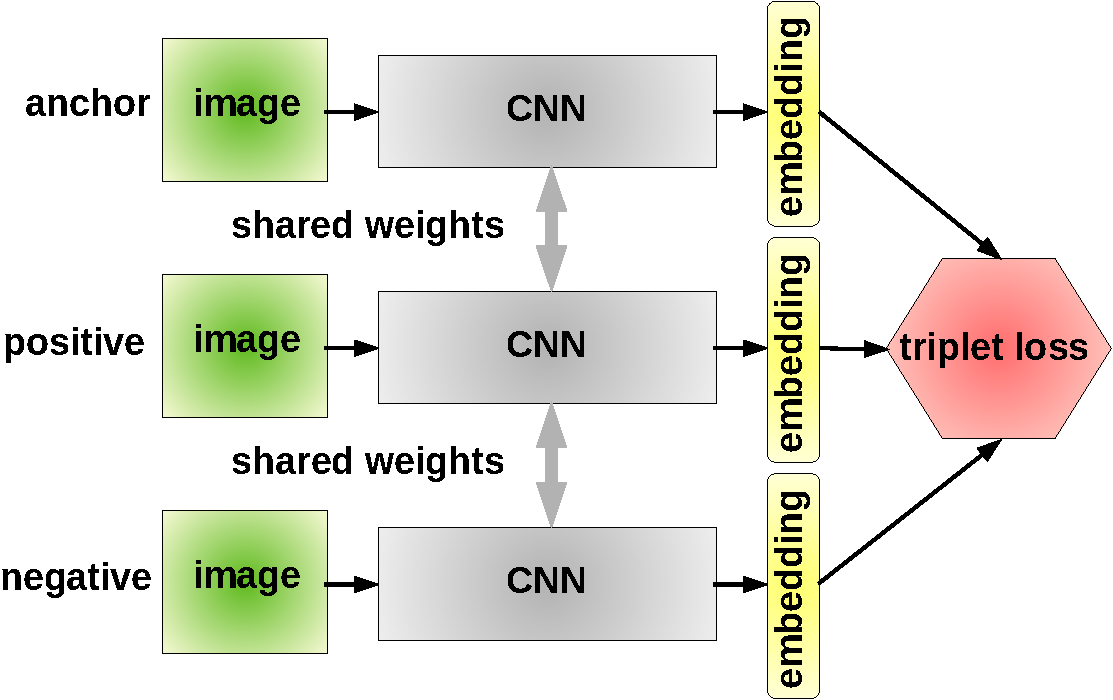
\includegraphics[width=\textwidth]{figures/theoretical_foundations/triplet_architecture.pdf}
        \caption[]{}
    \end{subfigure}
    \caption[Contrastive and triplet loss]{Comparison of the Siamese \imgpartdesc{a} and the triplet \imgpartdesc{b} network architectures. The concept of weight sharing implies that the same network is used for inference and only one set of weights is trained. Architectures are depicted as containing multiple models only for conceptual understanding.}
    \label{fig:SiameseAndTripletArchitectures}
\end{figure}

Let $\func{D}{x, y}: \mathbb{R}^D \times \mathbb{R}^D \to \mathbb{R}$ be a metric function measuring distances in the embedding space. Without a loss of generality, we resort to use of the Euclidean distance ($L_2$ norm), so $\func{D}{x, y} = \euclnorm{x - y}$.

\subsubsection{Contrastive Loss}

Consider a sample $\rbrackets{x_0, x_1, y}$, where $x_0$ and $x_1$ represent the input, and the label $y = 1$ if $x_0$ and $x_1$ belong to the same category, otherwise $y = 0$. $\func{D}{\cdot}$ is the previously defined metric function, and $\alpha$ is the margin representing the minimum distance in the metric space to separate positive from negative samples. Then the contrastive function for any sample is defined as~\cite{hadsell2006dimreduction}
\begin{equation}
    \label{eq:ContrastiveLoss}
    \func{\mathcal{L}_{contr}}{\theta} =
    \frac{1}{2}y
    {\func{D}{\func{f_\theta}{x_0}, \func{f_\theta}{x_1}}}^2 +
    \frac{1}{2}
    \rbrackets{1 - y} {\rbrackets{
            \sbrackets{\alpha - \func{D}{\func{f_\theta}{x_0}, \func{f_\theta}{x_1}}}_{+}}}^2.
\end{equation}
The two inputs $x_0$ and $x_1$ are fed to the shared model at the same time. The output is then evaluated by the contrastive loss function (\figstr{}~\ref{fig:SiameseAndTripletArchitectures} \imgpartdesc{a}). Positive samples should have a small distance between each other as measured by the $\func{D}{\cdot}$ to decrease the loss towards $0$. On the other hand, negative samples should have the distance beyond the threshold $\alpha$ to incur a loss of $0$.

\subsubsection{Triplet Loss}

\begin{figure}[t]
    \centerline{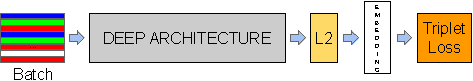
\includegraphics[width=0.8\linewidth]{figures/theoretical_foundations/triplet_loss_model_structure.pdf}}
    \caption[Triplet loss architecture]{A model structure developed by~\cite{schroff2015facenet}. This network consists of a batch input layer and a deep \gls{cnn} followed by an $L_2$ normalization, which produces the final embedding. A triplet loss is used during the training. \externalsrc{\cite{schroff2015facenet}}}
    \label{fig:TripletLossModelStructure}
\end{figure}

Apart from the contrastive loss, this time three samples are required to compute the loss. The rationale is to supply additional context when forming the metric space. Siamese networks are usually implemented using shared model weights, but there are better approaches when the triplet loss is used. Conceptually speaking, the model could be implemented as shown in \figstr{}~\ref{fig:SiameseAndTripletArchitectures} \imgpartdesc{b}. However, as we will discuss later, triplet mining strategies are required for the triplet loss to work properly. The model can be thus simplified from an architectural point of view at the cost of moving the complexity to the computation of the loss function (see \figstr{}~\ref{fig:TripletLossModelStructure}).

Let $N$ be the number of all possible valid triplets $\rbrackets{x_a^i, x_p^i, x_n^i}$ for a given dataset. For any $i$-th triplet, let $x_a^i$ be the \emph{anchor} for a specific object (person, vehicle, etc.) with label $\func{y}{x_a^i}$, $x_p^i$ be the positive sample of the same object with label $\func{y}{x_p^i}$, such that $x_a^i \neq x_p^i \land \func{y}{x_a^i} = \func{y}{x_p^i}$, and let $x_n^i$ with label $\func{y}{x_n^i}$ be a sample of any other object, satisfying $\func{y}{x_a^i} \neq \func{y}{x_n^i}$, $\forall i = 1, \dots, N$. Let $\alpha$ be the margin value that is enforced between positive and negative pairs. Then, we want the relationship~\cite{schroff2015facenet}
\begin{equation}
    \label{eq:TripletDistanceConstraint}
    \func{D}{\func{f_\theta}{x_a^i}, \func{f_\theta}{x_p^i}} + \alpha < \func{D}{\func{f_\theta}{x_a^i}, \func{f_\theta}{x_n^i}}, \forall i = 1, \dots, N,
\end{equation}
to hold true. The triplet loss function is therefore defined as~\cite{schroff2015facenet}
\begin{equation}
    \label{eq:TripletLoss}
    \func{\mathcal{L}_{triplet}}{\theta} =
    \sum_{i = 1}^{N}
    {\sbrackets{
        \alpha +
        \func{D}{\func{f_\theta}{x_a^i}, \func{f_\theta}{x_p^i}} -
        \func{D}{\func{f_\theta}{x_a^i}, \func{f_\theta}{x_n^i}}
    }}_+.
\end{equation}
During the training using the triplet loss, the model should learn to push negative samples further away from the positive samples, ideally exceeding the margin $\alpha$. Assuming a situation when the negative sample is mapped closer than a positive sample, the training should result in the desired situation of bringing the positive sample closer while pushing the negative one further (see \figstr{}~\ref{fig:TripletLossLearningProcess}).

\begin{figure}[t]
    \centerline{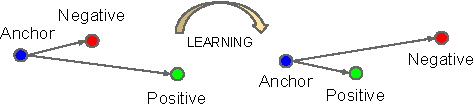
\includegraphics[width=0.7\linewidth]{figures/theoretical_foundations/triplet_loss_learning_process.pdf}}
    \caption[Triplet loss learning]{The objective is to learn embeddings such that the anchor is closer to the positive example than it is to the negative example by some specified margin value. The triplet loss, therefore, minimizes the distance between the anchor and the positive sample of the same identity and maximizes the distance between the anchor and the negative sample of a different identity. \externalsrc{\cite{schroff2015facenet}}}
    \label{fig:TripletLossLearningProcess}
\end{figure}

% ##############################################################################
\subsection{Triplet Mining Strategies}
\label{ssec:TripletMiningStrategies}

Contrastive (eq.~\ref{eq:ContrastiveLoss}) and triplet (eq.~\ref{eq:TripletLoss}) loss functions play an important role in training an embedding model. However, the way that pairs or triplets are selected is crucial and as Hermans~\etal{}~\cite{hermans2017triplet} and Manmatha~\etal{}~\cite{manmatha2017samplingmatters} showed, it may significantly influence the training. They demonstrated that the sampling strategy matters at least as much as the loss function itself. Moreover, as the dataset gets larger, then the number of possible triplets grows cubically, rendering the use of all of them impractical. The majority of those triplets would be so-called \emph{easy triplets}, thus hindering the learning process, because generating all possible triplets produces many triplets that fulfill the constraint \ref{eq:TripletDistanceConstraint}, hence provide inferior learning signal. To paraphrase the analogy from~\cite{hermans2017triplet}, showing the model that people with different clothes are not the same person after a certain point does not bring any new information. On the other hand, explicitly \emph{mining} images of similar-looking yet different people with the same clothes (\emph{hard negatives}) or of the same person with dramatically different poses (\emph{hard positives}) vastly contributes to an understanding of the notion of the \emph{same person}. As suggested, there are different kinds of triplets which are defined in the table \ref{tab:TripletCategoriesDefinitions}, using a general $\rbrackets{x_a^i, x_p^i, x_n^i}$ triplet for clarity. We encourage the reader to observe the figure \ref{fig:PositiveAndNegativeTripletsCategories}, too.

\begin{table}[t]
    \centering

    \begin{tabular}{|c|c|}
        \hline
        \tblcolname{triplet} & \tblcolname{constraint}                                                                                                                                            \\
        \hline

        easy                 &
        $\func{D}{\func{f_\theta}{x_a^i}, \func{f_\theta}{x_p^i}} + \alpha < \func{D}{\func{f_\theta}{x_a^i}, \func{f_\theta}{x_n^i}}$                                                            \\
        \hline

        semi-hard            &
        $\func{D}{\func{f_\theta}{x_a^i}, \func{f_\theta}{x_p^i}} < \func{D}{\func{f_\theta}{x_a^i}, \func{f_\theta}{x_n^i}} < \func{D}{\func{f_\theta}{x_a^i}, \func{f_\theta}{x_p^i}} + \alpha$ \\
        \hline

        hard                 & $\func{D}{\func{f_\theta}{x_a^i}, \func{f_\theta}{x_n^i}} < \func{D}{\func{f_\theta}{x_a^i}, \func{f_\theta}{x_p^i}}$                                              \\
        \hline
    \end{tabular}

    \caption{Definitions of various categories of triplets (regardless whether it is positive or negative) as imposed by their distance relationship.}
    \label{tab:TripletCategoriesDefinitions}
\end{table}

\begin{figure}[t]
    \centering
    \begin{subfigure}[b]{0.35\textwidth}
        \centering
        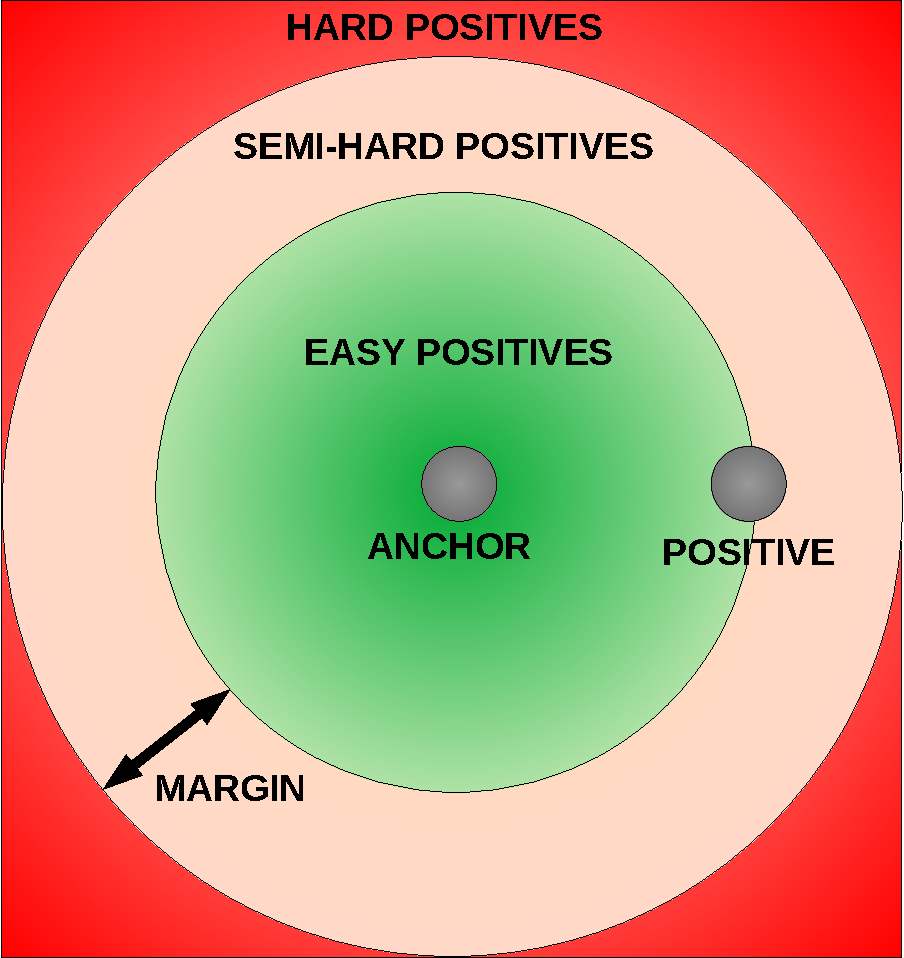
\includegraphics[width=\textwidth]{figures/theoretical_foundations/triplet_positives_categories.pdf}
        \caption[]{}
    \end{subfigure}
    \hfill
    \begin{subfigure}[b]{0.35\textwidth}
        \centering
        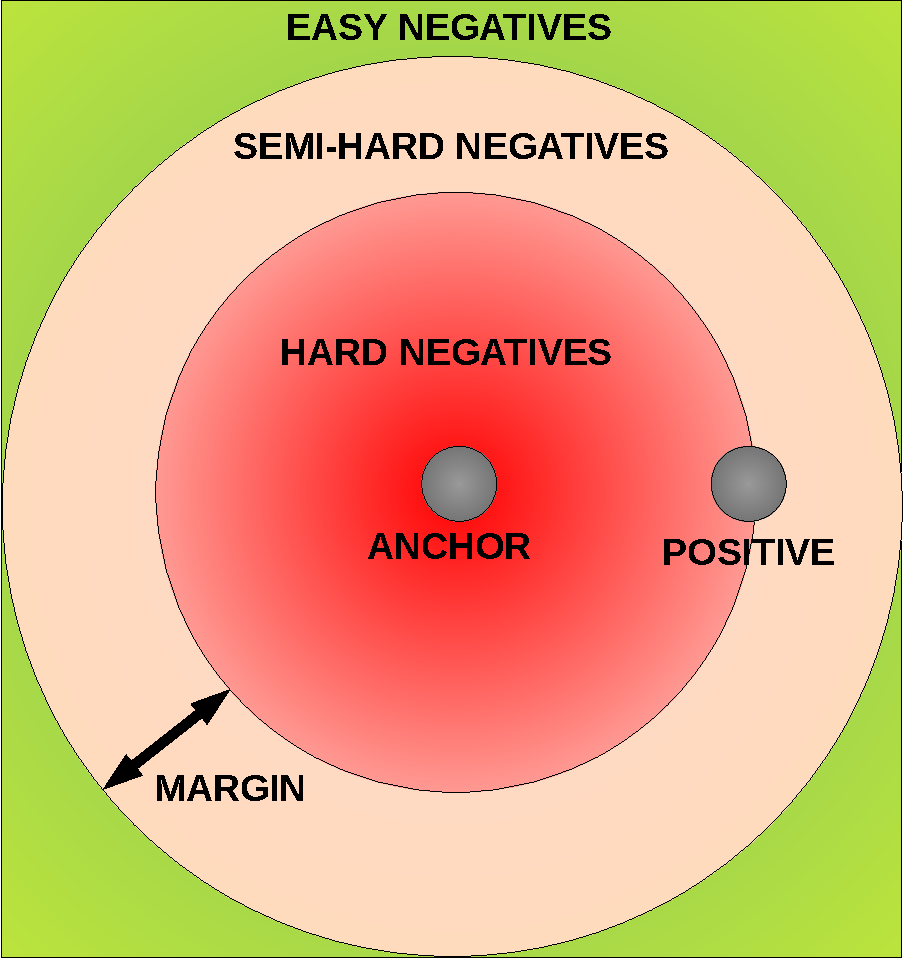
\includegraphics[width=\textwidth]{figures/theoretical_foundations/triplet_negatives_categories.pdf}
        \caption[]{}
    \end{subfigure}
    \caption[Triplet loss categories visualization]{Given a fixed anchor $x_a^i$ and positive sample $x_p^i$ as well as some positive margin value $\alpha$, we discriminate between three different types of categories in terms of their level of \emph{difficulty}. These categories vary in relation to positive \imgpartdesc{a} or negative \imgpartdesc{b} perspective.}
    \label{fig:PositiveAndNegativeTripletsCategories}
\end{figure}

In order to attain an effective convergence during the training, it is necessary to select triplets that violate the triplet constraint in eq. \ref{eq:TripletDistanceConstraint}. This means that given $x_a^i$, the goal is to select a \emph{hard positive} $x_p^i$ given by $\argmax_{x_p^i}\cbrackets{\func{D}{\func{f_\theta}{x_a^i}, \func{f_\theta}{x_p^i}}}$ and a \emph{hard negative} $x_n^i$ as a result of $\argmin_{x_n^i}\cbrackets{\func{D}{\func{f_\theta}{x_a^i}, \func{f_\theta}{x_n^i}}}$. Admittedly, it is often infeasible to compute the $\argmin\cbrackets{\cdot}$ and $\argmax\cbrackets{\cdot}$ over the entire training set. In this regard, there are two possible approaches to tackle this problem, either by selecting these hard triplets online or doing it offline~\cite{schroff2015facenet}.

\subsubsection{Offline Triplet Mining}

Given a training set, the task is to produce reasonable triplets off-line, for instance, at the epoch beginning. First, a list of $N$ different valid triplets is randomly generated, then separated into $\lfloor \nicefrac{N}{B} \rfloor$ batches of $B$ triplets, followed by computation of $3N$ embeddings using the most recent network checkpoint. Each sample in a batch consists of a triplet, so the embedding has to be computed three times. Subsequently, hard or semi-hard triplets may be selected. Since this strategy has been shown on multiple occasions~\cite{schroff2015facenet, hermans2017triplet, kuma2019vehiclereid} as an inferior choice compared to the online triplet mining, we will not discuss this approach further.

\subsubsection{Online Triplet Mining}

Online mining is performed by selecting the hard positive/negative exemplars from within a mini-batch (fig. \ref{fig:TripletArchitectureOnlineMining}). A condition that a minimum number of exemplars for any identity is present in each mini-batch has to be met. For example, Schroff et. al.~\cite{schroff2015facenet} used $40$ different images of a single person (an identity) per mini-batch. Let $P$ be the number of different objects/identities (people, vehicles, etc.) and $K$ be the number of different images for a concrete identity (e.g. different views of the same vehicle). There are two prominent approaches to online mining: \emph{batch all} and \emph{batch hard}.

\begin{figure}[t]
    \centerline{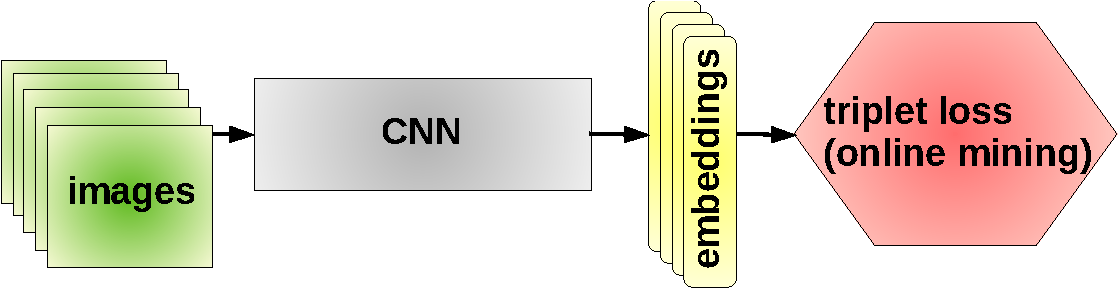
\includegraphics[width=0.55\linewidth]{figures/theoretical_foundations/triplet_architecture_online_mining.pdf}}
    \caption[Triplet loss online mining architecture]{The architecture of a triplet network where an online triplet loss function is used for training. In this architecture, no weight sharing is required as the triplet selection happens \emph{online} solely in the loss function.}
    \label{fig:TripletArchitectureOnlineMining}
\end{figure}

\subsubsection{Online Triplet Mining: Batch All}

This strategy aims for selecting all valid triplets and averaging the loss only on the hard and semi-hard triplets. Easy triplets, i.e., those for which the loss function equals $0$), are not taken into account. The reason is that averaging on them would result in a very small loss, since they would usually vastly outnumber the set of harder triplets~\cite{hermans2017triplet}. This approach produces a total of $PK \rbrackets{K - 1} \rbrackets{PK - K}$ triplets ($PK$ anchors, $K - 1$ positives per anchors, $PK - K$ negatives) incorporated in the loss function as
\begin{equation}
    \label{eq:BatchAllLossFunction}
    \begin{aligned}
        \func{\mathcal{L}_{batchall}}{\theta} =
        \sum_{i = 1}^P
        \sum_{a = 1}^K
        \sum_{\substack{p = 1 \\p \neq a}}^K
        \sum_{\substack{j = 1 \\j \neq i}}^P
        \sum_{n = 1}^K
        \Bigg[
         & \alpha +           \\
         & \func{D}{
            \func{f_\theta}{x_a^i},
            \func{f_\theta}{x_p^i}
        } -                   \\
         & \func{D}{
            \func{f_\theta}{x_a^i},
            \func{f_\theta}{x_n^j}
        }
        {\Bigg]}_{+}.
    \end{aligned}
\end{equation}

\subsubsection{Online Triplet Mining: Batch Hard}

In this strategy, the goal is to find the hardest positive and hardest negative for each anchor. The total number of triplets is $PK$. The selected triplets are the hardest among the given batch~\cite{hermans2017triplet}. Additionally, Hermans~\etal{}~\cite{hermans2017triplet} say that the selected triplets can be considered moderate, since they are the hardest within a small subset of the data, which is the best for learning with the triplet loss.
\begin{equation}
    \begin{aligned}
        \func{\mathcal{L}_{batchhard}}{\theta} =
        \sum_{i = 1}^P
        \sum_{a = 1}^K
        \Bigg[
         & \alpha +                            \\
         & \underset{p = 1, \dots, K} {\max}
        \cbrackets{
            \func{D}{
                \func{f_\theta}{x_a^i},
                \func{f_\theta}{x_p^i}
            }
        } -                                    \\
         & \underset{\substack{j = 1, \dots, P \\n = 1, \dots, K\\j \neq i}} {\min}
        \cbrackets{
            \func{D}{
                \func{f_\theta}{x_a^i},
                \func{f_\theta}{x_n^j}
            }
        }
        {\Bigg]}_{+}
    \end{aligned}
\end{equation}

% ##############################################################################
\subsection{Training Embeddings Using Adversarial Learning}
\label{ssec:TrainingEmbeddingsAdversarialLearning}

As we have seen so far, the mining of \emph{hard} samples (pairs or triplets) is crucial for training the embedding model. Nevertheless, as the model improves, it is mandatory to provide \emph{harder} samples every time. It can be observed in the contrastive (equation~\ref{eq:ContrastiveLoss}) or the triplet loss (equation~\ref{eq:TripletLoss}) functions. Once the negative sample is \emph{pushed} beyond the margin boundary, this sample incurs a $0$ contribution to the loss. It, therefore, is appropriate to constantly provide \emph{harder} samples as the model progresses, but the number of hard samples within the training set naturally decreases. One way to achieve this is to utilize adversarial training, the concept introduced by Goodfellow~\etal{}~\cite{goodfellow2014gans}. An architecture called the Embedding Adversarial Learning Network, proposed by Lou~\etal{}~\cite{lou2019embreid} is capable of generating synthetic samples in the embedding space. The advantage of harnessing this scheme is that instead of mining abundant \emph{hard} samples from the training set, which may be remarkably laborious, if not impossible, the automatically generated \emph{hard} samples can greatly improve the network's capability for discriminating similar objects~\cite{lou2019embreid}. Since Lou~\etal{}~\cite{lou2019embreid} also deal with the problem of vehicle \gls{reid}, their approach improves the robustness of the embedding model to queries with different views of vehicles, because they employ \emph{hard negative} mining and \emph{cross-view} generation during the training. Identification of the corresponding rear viewpoint of a vehicle given only its front viewpoint and vice versa casts a challenge for the \gls{reid} methods.

Their contribution encompasses a novel adversarial scheme based on feature distance within the embedding space. Following the notation from~\cite{lou2019embreid}, let $x$ be an input sample, and $\func{G}{x}$ be a generated sample using the generator $G$. $\func{G}{x}$ is constrained to be close to the given sample $x$, within a relative positive margin $\alpha$, in the target embedding space. On the contrary, let $D_{emb}$ be the discriminator the purpose of which is to push the $\func{G}{x}$ away from $x$ while aiming to make the relative distance to be greater than $\alpha$. Simply put, the generator $G$ attempts to minimize the feature distance while the discriminator $D_{emb}$ tries to maximize it (\figstr{}~\ref{fig:EALNDiscriminatorGeneratorScheme}). This adversarial scheme can be formulated as follows,
\begin{equation}
    \begin{aligned}
         & \underset{G}{\min} \ \underset{D_{emb}}{\max} \ \mathbb{E}_{x \sim \func{pdata}{x}} \max \cbrackets{\func{d}{x, \func{G}{x}} - \alpha, 0}, \\
         & \func{d}{x, \func{G}{x}} = \euclnorm{\func{D_{emb}}{x} - \func{D_{emb}}{\func{G}{x}}}^2,
    \end{aligned}
\end{equation}
with $\func{D_{emb}}{x}$ being the mapping of $x$ to the embedding space through the discriminator $D_{emb}$~\cite{lou2019embreid}. As~\cite{goodfellow2014gans} proposed in his initiative work on \glspl{gan}, the generator and the discriminator are trained alternatively in this scheme as well.

\begin{figure}[t]
    \centerline{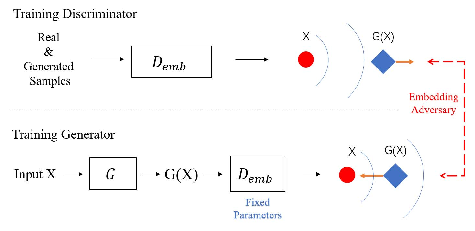
\includegraphics[width=0.8\linewidth]{figures/theoretical_foundations/ealn_discriminator_generator_scheme.pdf}}
    \caption[Embedding adversarial learning architecture]{Adversarial learning between the generator $G$ and the discriminator $D_{emb}$. The generator $G$ tries to produce samples close to the given sample $x$ in the embedding space, while the discriminator $D_{emb}$ tries to push those samples far away from each other, beyond the margin $\alpha$~\cite{lou2019embreid}.}
    \label{fig:EALNDiscriminatorGeneratorScheme}
\end{figure}

Their approach encompasses multiple stages. The first one is the \emph{embedding adversarial learning}, the design principle of which is manipulating the generation of the samples in the embedding space. Later on, the aforementioned first stage is extended by the \emph{hard negative adversarial learning}, that consists of two parts, i.e., the \emph{embedding adversarial learning} and the \emph{real-fake adversarial learning}. Another concurrent stage is introduced, called the \emph{cross-view adversarial learning}. Based on the \emph{embedding adversarial learning}, the aim is to address the issue of vehicle feature matching between different views via cross-view generation.

\section{Evaluating Information Retrieval}
\label{sec:EvaluatingInformationRetrieval}

% ##################################################
\subsection{Elementary Measures of Classification}
\label{ssec:ElementaryMeasuresOfClassification}

In order to put the meaning of \gls{map} (section~\ref{ssec:MeanAveragePrecision}) into a broader context, we will briefly explain the basics of accuracy, precision, recall, and some other derived metrics. We will use the standard terminology to denote whether the classification is correct (true) or not (false), for both positive and negative categories. All these measures can be obtained from the confusion matrix (see table \ref{tab:ConfusionMatrix}).

\begin{table}[t]
    \centering
    
    \begin{tabular}{|c|c|c|}
        \hline
                                        & \tblcolname{Actual positive} & \tblcolname{Actual negative}\\
        \hline
        \tblcolname{Predicted positive} & \gls{tp}                     & \gls{fp}\\
        \hline
        \tblcolname{Predicted negative} & \gls{fn}                     & \gls{tn}\\
        \hline
    \end{tabular}
    
    \caption[Confusion matrix]{A confusion matrix in the standard form. \externalsrc{\cite{Davis2016}}}
    \label{tab:ConfusionMatrix}
\end{table}

\begin{table}[t]
    \centering
    
    \begin{tabular}{|p{0.2\linewidth}|p{0.2\linewidth}|p{0.5\linewidth}|}
        \hline
            
        \tblcolname{Measure} & \tblcolname{Formula} & \tblcolname{Description}\\
        \hline
        
        accuracy &
        $\frac{\TP + \TN}{\TP + \TN + \FP + \FN}$ &
        percentage of all the correct outcomes, a measure of statistical bias (systematic errors)\\
        \hline
        
        precision &
        $\frac{\TP}{\TP + \FP}$ &
        the percentage of predictions that are correct, useful when the costs of \gls{fp} are high\\
        \hline
        
        recall &
        $\frac{\TP}{\TP + \FN}$ &
        a.k.a sensitivity, it's the percentage of correctly spotted positives, useful when the costs of \gls{fn} are high\\
        \hline
        
        true positive rate &
        $\frac{\TP}{\TP + \FN}$ &
        equal to recall\\
        \hline
        
        false positive rate &
        $\frac{\FP}{\FP + \TN}$ &
        the percentage of negative instances incorrectly classified as positives (\gls{fp}), often referred to as \emph{alarm rate}\\
        \hline
        
        positive predictive value &
        $\frac{\TP}{\TP + \FP}$ &
        equal to precision\\
        \hline
    \end{tabular}
    
    \caption[Measures of binary classification]{Elementary measures for evaluating binary classification. \externalsrc{\cite{Davis2016}}}
    \label{tab:ElementaryMetrics}
\end{table}

% ##################################################
\subsection{Important Curves}
\label{ssec:ImportantCurves}

\subsubsection{Precision-Recall Curve}
\label{sssec:PrecisionRecallCurve}

The precision-recall curve summarizes the trade-off between precision and recall for a given predictive model using different thresholds of probability. The precision-recall curve is appropriate for imbalanced datasets, i.e., datasets where the number of instances in each class may differ considerably (large skew in the class distribution~\cite{Davis2016}).

\subsubsection{ROC Curve}

\cite{James2013} describes the \gls{roc} curve as simultaneously displaying two types of errors for all possible thresholds. It summarizes the trade-off between the true positive rate and false positive rate for a given predictive model using different thresholds of probability. The overall performance of a classifier is given by the \gls{auc} of the \gls{roc}. This curve is appropriate to use when the observations are balanced between each class in terms of the number of occurrences (as opposed to the aforementioned precision-recall curve).

% ##################################################
\subsection{Evaluating Bounding Box Prediction}
\label{ssec:EvaluatingBoundingBoxPrediction}

\subsubsection{Intersection Over Union}
\label{sssec:IntersectionOverUnion}

\glslocalreset{iou}

\Gls{iou} measures the overlap between two boundaries. For our purposes, we will use \gls{iou} as a quantitative measure of overlap between two \glspl{bbox}, where one is the ground truth \gls{bbox} and the other is the predicted one (see figure \ref{fig:IntersectionOverUnion}).

Let $\supsub{\vect{b}}{1}{T} = \sbrackets{x_1, y_1, w_1, h_1}$ and $\supsub{\vect{b}}{2}{T} = \sbrackets{x_2, y_2, w_2, h_2}$ be two \glspl{bbox}, not necessarily different, described by vectors containing $4$ integer elements. The respective elements are given by $x$, $y$ coordinates of the top-left corner as well as the \gls{bbox} width and height. The intersection area between $\vect{b}_1$ and $\vect{b}_2$ is defined as
\begin{equation}
\begin{aligned}
    \vect{b}_1 \cap \vect{b}_2 =
    &\max \cbrackets{0,
                    \min \cbrackets{x_1 + w_1, x_2 + w_2} - \max \cbrackets{x_1, x_2} + 1}
    \times\\
    &\max \cbrackets{0,
                    \min \cbrackets{y_1 + h_1, y_2 + h_2} - \max \cbrackets{y_1, y_2} + 1},
\end{aligned}
\end{equation}
and the area of their union is given by
\begin{equation}
    \vect{b}_1 \cup \vect{b}_2 = w_1 h_1 + w_2 h_2 - \vect{b}_1 \cap \vect{b}_2.
\end{equation}
Then, the final \gls{iou} metric between $\vect{b_1}$ and $\vect{b_2}$ is computed as
\begin{equation}
    \label{eq:IntersectionOverUnion}
    \func{\IOU}{\vect{b}_1, \vect{b}_2} =
    \frac{\vect{b}_1 \cap \vect{b}_2}{\vect{b}_1 \cup \vect{b}_2},
\end{equation}
where $0 \leq \func{\IOU}{\vect{b}_1, \vect{b}_2} \leq 1$, such that value of $0$ represents no intersection, while value of $1$ represents a complete overlap. In terms of object detection or object tracking evaluation, an \gls{iou} threshold, $t$, such that $0 \leq t \leq 1$, can be associated with this metric, denoting the decision boundary whether the prediction is a \gls{tp} or a \gls{tn}.

\begin{figure}[t]
    \centerline{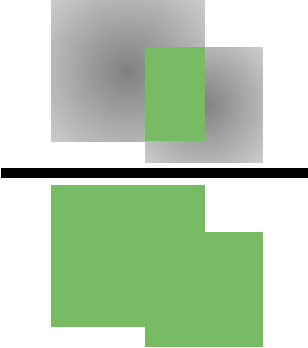
\includegraphics[width=0.25\linewidth]{figures/theoretical_foundations/intersection_over_union.pdf}}
    \caption[\Gls{iou} visualization]{Computation of the \gls{iou} metric between two \glspl{bbox} using of ratio of the area of overlap and the area of the union.}
    \label{fig:IntersectionOverUnion}
\end{figure}

% ##################################################
\subsection{Mean Average Precision}
\label{ssec:MeanAveragePrecision}

\glslocalreset{map}

\Gls{map} belongs to commonly used approaches for evaluation of tracking algorithms, document searching systems, object detection, object \gls{reid}, and many others. Generally speaking, it measures the success rate of an information retrieval algorithm. Such evaluation measures are used to determine how well the search results satisfied the user's query intent. This metric is often associated with popular datasets and their respective annual challenges, for instance, PASCAL \gls{voc}~\cite{Everingham10} and MS \gls{coco}~\cite{Lin2014} challenge.

\subsubsection{Object Re-Identification}
\label{sssec:ObjectReIdentification}

A common use case in the context of object \gls{reid} is to use \gls{map} to assess the search results for a particular query using Euclidean distance or cosine similarity as a metric. Oftentimes the model is trained with intent to use one of these trivial metrics. Furthermore, this approach is often paired with \emph{top-k} accuracy, typically \emph{top-1}, \emph{top-2} and \emph{top-5}.

In a typical \gls{reid} evaluation setup, there is a query set and a so-called gallery set. For each object in a query set the aim is to retrieve a similar identity from the test set (i.e. the gallery set). The computation of the \gls{ap} for a query image $q$ is thus defined as
\begin{equation}
    \label{eq:AveragePrecision}
    \func{\AP}{q} = \frac{1}{\func{N_{gt}}{q}} \sum_{k} \func{P}{k} \times {\delta}_k,
\end{equation}
where $\func{P}{k}$ represents precision at rank $k$, $\func{N_{gt}}{q}$ is the total number of true retrievals for the query $q$. The indicator ${\delta}_k$ is equal to $1$ when the matching of query image $q$ to a test image is correct at rank $r$, such that $1 \leq r \leq k$. The \gls{map} is then calculated as average over all query images, concretely
\begin{equation}
    \label{eq:MeanAveragePrecision}
    \MAP = \frac{1}{Q} \sum_q \func{\AP}{q},
\end{equation}
where $Q$ is the total number of query images, as described in~\cite{Kuma2019}. The equation \ref{eq:MeanAveragePrecision} essentially tells us is that, for a given query $q$, we calculate its corresponding \gls{ap} (defined in equation \ref{eq:AveragePrecision}), and then take the mean of the all these \gls{ap} scores, quantifying how well our model responds to the query $q$.

\subsubsection{Object Detection}

Object detection models seek to identify the presence of objects in images and then classify them. The evaluation metric of such a model has to take the \gls{bbox} prediction into account, as there can be just a partial overlap of the predicted \gls{bbox} with the ground truth one. Even though we defined \gls{map} for object \gls{reid} (section \ref{sssec:ObjectReIdentification}), the \gls{map} is also used for object detection, and its definition was initially formalized in the PASCAL \gls{voc} challenge~\cite{Everingham10}, which consisted of various tasks involving image processing demanding robust evaluation metrics.

In a ranked retrieval context, appropriate sets of retrieved documents are naturally given by the \emph{top-k} retrieved documents and for each such set, the precision-recall curve (section \ref{sssec:PrecisionRecallCurve}) can be plotted~\cite{salton_introduction_1983}. With this in mind, recall is defined as the proportion of all positive examples ranked above a given rank. Precision is the proportion of all examples above that rank which are from the positive class. In~\cite{Everingham10}, the \gls{ap} is computed for $11$ equally spaced discrete recall levels, specifically $\sbrackets{0.0, 0.1, 0.2, \dots, 1.0}$, using
\begin{equation}
    \AP = \frac{1}{11} \sum_{r \in \cbrackets{0.0, 0.1, \dots, 1.0}} \func{p_{interp}}{r},
\end{equation}
where the precision at each recall level $r$ is interpolated by taking the maximum precision measured for a method for which the corresponding recall exceeds $r$. Precision interpolation is used to remove the \emph{zig-zag} pattern by evaluating
\begin{equation}
    \func{p_{interp}}{r} = \underset{\tilde{r}:\tilde{r} \geq r}{\max} \quad \func{p}{\tilde{r}},
\end{equation}
with $\func{p}{\tilde{r}}$ representing the measures precision at a specific recall level $\tilde{r}$~\cite{Everingham10, salton_introduction_1983}.

\section{Evaluating Visual Object Tracking}
\label{sec:EvaluatingVisualObjectTracking}

In our work, we tackle problems of \Gls{vot}, concretely \gls{mot}, for which there are no established solutions neither for prediction itself nor for its evaluation. The research is practically still ongoing. When it comes to evaluating \gls{mot} performance, even after many years, there is still no consensus how to approach the evaluation and subsequent comparison of multi-object trackers~\cite{bernardin2008clearmot}.

There is one established metric, however, called \gls{clear} \gls{mot} metric~\cite{bernardin2008clearmot} (further referred to as just \gls{clear}), that we will employ to evaluate and quantitatively assess the performance of a \gls{mot} system. The reasons are the following:
\begin{itemize}
    \item This metric is still considered a reasonably effective and intuitive metric to use, despite multiple proposals for improvements~\cite{wen2020uadetrac}.
    \item Numerous works in object tracking, especially tracking of people, report statistics from the \gls{mot} challenges that historically have utilized this metric.
    \item From the engineering perspective, there are standard frameworks (e.g.,~\cite{webpymotmetrics}) that provide evaluation of a custom \gls{mot} tracker inference with a plethora of configurations and additional metrics as a bonus that make peeking into the performance of the tracker a lot easier. For instance, we were particularly interested in additional metrics such as the number of object switches (explained later) etc.
\end{itemize}

Bernardin~\etal{}~\cite{bernardin2008clearmot}, the authors of \gls{clear} discussed above, designed two crucial criteria that performance metrics should meet. Here we present their list in which the first two items are considered primary, whereas the remaining are expected properties of useful metrics, but not necessarily demanded. Therefore, such metrics should:
\begin{enumerate}
    \item allow to assess the tracker's precision regarding how well it is capable of determining the exact object location,
    \item reflect the tracker's ability to track objects consistently, i.e., to correctly trace object trajectories such that one and only one trajectory is established per object,
    \item have as few free parameters as possible,
    \item be clear and easy to interpret while emphasizing intuitive human understanding of the tracking process,
    \item be general enough so that comparison of different types of trackers, e.g. $2$D or $3$D, is possible,
    \item contain expressive values rich in information yet not abundant in quantity.
\end{enumerate}

Considering this, they proposed a systematic approach to evaluating tracker's characteristics. For clarity, we will adopt the notation and nomenclature introduced in~\cite{bernardin2008clearmot}.

Let $t$ denote a time for a specific frame. For each frame $t$, the multi-object tracker produces a set of hypotheses $\cbrackets{h_1, h_2, \dots, h_m}$ for a set of visible objects $\cbrackets{o_1, o_2, \dots, o_n}$. With this in mind, the evaluation procedure can be briefly described in the following pseudocode.

For each time frame $t$:
\begin{enumerate}
    \item establish the best possible correspondence between hypotheses $h_i$ and objects $o_j$, where $i = 1, 2, \dots m$ and $j = 1, 2, \dots, n$,
    \item for each determined correspondence between object and hypothesis:
          \begin{enumerate}
              \item quantify the error in estimation of the object's position,
          \end{enumerate}
    \item perform accumulation of all errors (see \figstr{}~\ref{fig:CLEARHypotheses}) in the found correspondences:
          \begin{enumerate}
              \item count all false negatives (misses), i.e., objects for which there was no hypothesis,
                    item count all false positives, i.e., hypotheses for which there was no object,
                    item count mismatch errors (swaps of object IDs), i.e., situations in which the hypothesis for a given object changed compared to the previous frame.
          \end{enumerate}
\end{enumerate}

% ------------------------------------------------------------------------------
\begin{figure}[t]
    \centerline{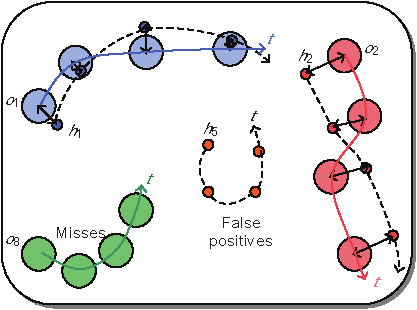
\includegraphics[width=0.55\linewidth]{figures/theoretical_foundations/clear_hypotheses_status.pdf}}
    \caption[\gls{clear} hypotheses]{With a demonstration of a correct tracker inference at the top, the \gls{clear} \gls{mot} metric distinguishes between three fundamental types of errors, misses (false negatives), false positives and ID switches, shown in this order respectively. \externalsrc{\cite{bernardin2008clearmot}}}
    \label{fig:CLEARHypotheses}
\end{figure}

% ##############################################################################
\subsection{Establishing Correspondences}

The correspondence between a hypothesis $h_i$ and an object $o_j$ should not be made unless their distance (denoted as $d_{i,j}$) is within a specific threshold $T$. The measure of distance has to be defined for each task, but the \gls{iou} distance or Euclidean distance of \gls{bbox} centroids are most commonly used. From now on, we define object-hypothesis correspondence to be valid as long as $d_{i,j} < T$.

The value of $T$ is critical and greatly influences the outcome. Evaluating tracking performance bears the burden of having parameters that are difficult to generalize and the process of setting their values is often accompanied with experimentation. For example, conceptually speaking, there is by all means a boundary (the threshold $T$) beyond which we can no longer speak of an error in position estimation, but rather we could claim that the tracker has drifted away and is tracking a completely different object. With that being said, the exact value of this boundary is up for a discussion.

% ##############################################################################
\subsection{Tracking Consistency}

In order to properly examine the tracker in terms of how consistent it is at tracking objects, one has to detect conflicting predictions for the given object over time. We acknowledge that there may be numerous approaches to this problem. Bernardin~\etal{}~\cite{bernardin2008clearmot} remarked that such procedures somehow need to decide what the ``best'' mapping is. For instance, assuming an object $o_j$ and a hypothesis $h_i$, the ``optimal'' matching may be based on the initial correspondence made for $o_j$ or the most frequent correspondence made throughout the whole sequence. If any violation is encountered, it is then treated as a discrepancy and thus counted as error.

However, there are several issues with such approaches. Consider scenarios depicted in \figstr{}~\ref{fig:SeqLevelMostCommonCorrespondenceProb}. The authors raised their concerns regarding the objectivity of such evaluation and proposed a slightly different method. They only count mismatch errors once at the time frame where the change occurrs, and consider the remaining intermediate correspondences as correct. We agree with such objection, since local discrepancy in object-hypothesis correspondence may indicate just a temporary drift the tracker, whereas its ability to preserve the object's identity does not necessarily have to be so poor as the original metric would display.

Let $M_t = \cbrackets{\rbrackets{h_i, o_j}}$ be the set of mappings made up to time $t$, such that $M_0 = \cbrackets{\cdot}$. Once a new correspondence is made at the next step at time $t + 1$ between the hypothesis $h_k$ and the object $io_j$ that conflicts the already established identity by the pair $\rbrackets{h_i, o_j}$ in $M_t$, this contradition is then counted as a mismatch error and $\rbrackets{h_i, o_j}$ is replaced by $\rbrackets{h_k, o_j}$ in $M_{t + 1}$. Consequently, papping that is constructed this way enhances decision-making when facing multiple competing hypotheses for the same object. The implicit assumption is that the previously assigned hypothesis is more likely to be correct that the new one, even if the distance metric alone would indicate otherwise (see \figstr{}~\ref{fig:ObjectHypothesisReInit} for illustration).

% ------------------------------------------------------------------------------
\begin{figure}[t]
    \centerline{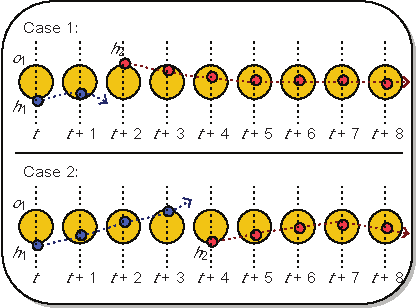
\includegraphics[width=0.5\linewidth]{figures/theoretical_foundations/seq_based_correspondence_issues.pdf}}
    \caption[Sequence-based correspondence mismatches]{This figure illustrates the inherent ``unfairness'' when relying on sequence-level ``best'' object-hypothesis mapping induced by the most frequent correspondence. As shown in the case $1$, the correct hypothesis is the $h_2$, and thus only $2$ errors are incurred for the first mismatch. The case $2$ is practically identical, the $h_2$ also represents the most common assignment. However, $4$ errors are accumulated for the alleged mismatch for $h_1$. \externalsrc{\cite{bernardin2008clearmot}}}
    \label{fig:SeqLevelMostCommonCorrespondenceProb}
\end{figure}

% ------------------------------------------------------------------------------
\begin{figure}[t]
    \centerline{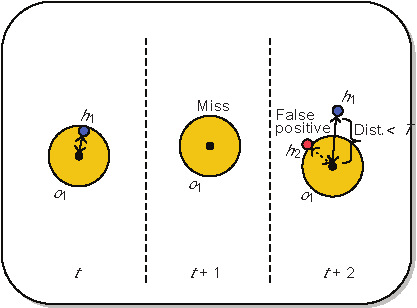
\includegraphics[width=0.5\linewidth]{figures/theoretical_foundations/object_hypothesis_reinit.pdf}}
    \caption[Object-hypothesis re-initialization]{Demonstration of a track reinitialization. At time $t$, the identity of the object $o_1$ is accounted for by the hypothesis $h_1$. At time $t + 1$, the object disappears and the track is temporarily lost. At time $t + 2$, the tracker is responsible for reinstantiating the object identity. During evaluation, the underlying assumption is that the previous hypothesis should be the correct one, even if the new hypothesis is closer according to the used distance function. \externalsrc{\cite{bernardin2008clearmot}}}
    \label{fig:ObjectHypothesisReInit}
\end{figure}

% ##############################################################################
\subsection{Mapping Procedure}

In what follows, we will describe a recipe for the mapping procedure based on the previously discussed foundations.

Let $M_0 = \cbrackets{\cdot}$. For each time frame $t$:
\begin{enumerate}
    \item Verify if every mapping in $\rbrackets{h_i, o_j}$ in $M_{t - 1}$ is still valid. Such pair is deemed valid as long as the hypothesis $h_i$ exists at time $t$, the object $o_j$ is still visible while the distance between the two does not exceed $T$. If these conditions hold, establish a correspondence.
    \item If there are objects for which no correspondence has been made so far, then a suitable matching hypothesis is searched for. This step involves one-to-one matching for pairs the distance of which does not exceed the threshold $T$. The matching procedure is formulated as minimum cost assignment problem and Munkres's algorithm~\cite{munkres1957assignment} can be adopted. In case there happens to be a correspondence that contradicts a mapping $\sbrackets{h_i, o_j}$ as part of $M_{t - 1}$, then replace the previous pair $\sbrackets{h_i, o_j}$ with $\sbrackets{h_k, o_j}$ and treat such an occurrence as a mismatch error. For simplicity, let $mme_t$ be the number of the mismatch errors for the frame $t$.
    \item The two previous steps guaratee that a complete set of matching pairs has been generated for the current time $t$. At this point, we may start calculating values that will be utilized later on for computing the final metrics. So, let $c_t$ be the number of matches found for time $t$. For each such match, compute the distance (once again, up to the designer's choice) between the object $o_j$ and the corresponding hypothesis, denoted by $d_{ti}$.
    \item Every hypothesis that is not part of any pair up to this point is reckoned as false positive. Likewise, all the remaining objects are marked as misses, i.e., false negatives. Thus, let $fp_t$ and $m_t$ be the number of false positives and misses, respectively. For sakes of computation, let us define $g_t$ as the number of ground-truth objects visible at time $t$.
\end{enumerate}

Please note that no mismatch errors can occurr at the initial frame as the set of mappings $M_0$ is empty and therefore all correspondences are treated as initializations.

% ##############################################################################
\subsection{Performance Metrics}

In light of the previously described procedure and introduced notation, here we present the two most relevant performance metrics by which the tracking performance can be intuitively expressed using two quantities, namely the ``tracking precision'' and ``tracking accuracy''. Even though it could be argued whether such expression is sufficient.

In general terms, the role of tracking precision is to measure the alignment between the predicted object position (e.g., its \gls{bbox}) and the groud-truth position only for the positive sample. With that being said, precision is not influenced by the ability (or lack thereof) of the tracker to detect objects properly. It is designed to evaluate the suitability of the delineation of the object \gls{bbox} the detection of which was correct in the first place. The \gls{motp} metric can thus be defined as
\begin{equation}
    \label{eq:MOTPMetric}
    \text{MOTP} = \frac{\sum_{\forall t} \sum_{\forall i} d_{ti}}{\sum_{\forall t} c_t},
\end{equation}
\eqstr{}~\ref{eq:MOTPMetric} represents the total error in the estimated position for the pairs where the object-hypothesis relationship was correctly determined averaged over the total number of such matches made. As stated above, it gauges the ability of the tracker to estimate precise object positions regardless of its capability of recognizing them or keeping their trajectories consistent.

Conversely, the accuracy metric attempts to reflect the number of mistakes the tracker made in terms of misses, false positives, object mismatches, failures to recover already established tracks, and so forth. Given this description, the \gls{mota} metric can be expressed as
\begin{equation}
    \label{eq:MOTAMetric}
    \text{MOTA} = 1 - \frac{\sum_{\forall t} \rbrackets{m_t + fp_t + mme_t}}{\sum_{\forall t} g_t},
\end{equation}
the possible values of which lie within the interval $\sbrackets{-\infty, 1}$. For example, if a tracker produces a lot of false positives, the value in the sum may actually exceed one, and therefore, the final metric would be negative.

We would like to emphasize that the errors have to be first summed up across all the frames before computing the ratios rather than evaluating the ratio locally. Independent computation of the given ratios (in both equations~\ref{eq:MOTPMetric}~and~\ref{eq:MOTAMetric}) would lead to non-intuitive outcome (see \figstr{}~\ref{fig:LocalGlobalRatioEval} for details).

% ------------------------------------------------------------------------------
\begin{figure}[t]
    \centerline{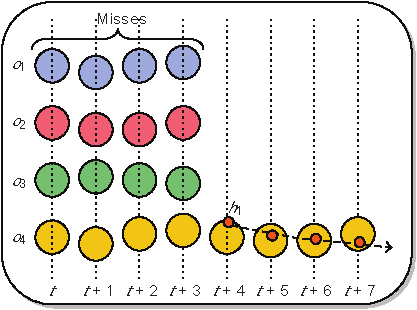
\includegraphics[width=0.6\linewidth]{figures/theoretical_foundations/local_vs_global_ratio_evaluation.pdf}}
    \caption[Local vs. global ratio evaluation]{Computing of error ratios needs to be performed on a global level, rather than on a local, frame level. Assume a sequence consisting of $8$ frames. Moreover, assume that objects $o_1, \dots, o_4$ are visible on the frames from $t_1$ to $t_4$, but none of them is being tracked. The situation changes at frame $t_4$ where only the object $o_4$ is being tracked properly by the hypothesis $h_1$. As a result, in frames $t_1, \dots, t_4$, the resulting miss rate is $100\%$, whereas in frames $t_5, \dots, t_8$ it is exactly $0\%$. Applying arithmetic average to these values yields a global miss rate of $\frac{1}{8} \rbrackets{4 \cdot 100 + 4 \cdot 0} = \frac{1}{2}$, or, $50\%$. Conversely, performing summation prior to quantifying the final global ratio produces far more intuitive result of $16$ out of $20$ misses, or the miss rate of $80\%$. \externalsrc{\cite{bernardin2008clearmot}}}
    \label{fig:LocalGlobalRatioEval}
\end{figure}

\section{Predicting Motion}
\label{sec:PredictingMotion}

To track objects in a video, there is a requirement to resolve the object's position in two consecutive frames. An ineffective brute-force approach would be to exploit the matching technique in the pixel space of the entire image, imposing an extreme computational overhead~\cite{Jalal2012}. Generally speaking, it is safe to assume that the object does not change its position abruptly. In case of vehicles, this is even more so. Tracking a jumping ball in a room that is constantly bouncing off the walls presents a greater challenge in terms of sudden change in trajectory than tracking a vehicle. Given this assumption, a physical model of the object can be utilized to reduce the region in the frame where the object should be searched for. Moreover, having a physical model backing up the visual tracking is essential as it may help determine potential failure if predictions of physical as well as visual models do not match up to a specific degree of confidence.

As we have mentioned numerous times, occlusion handling is of primary concern for us, and being able to predict a probability distribution over possible object's positions if visual input is absent is vital. We could potentially use filtering approaches, specifically Kalman filter (section~\ref{ssec:KalmanFiler}) or particle filter (section~\ref{ssec:ParticleFilter}) described later. These algorithms could model the vehicle's speed and acceleration. Filtering is an engineering terminology describing the extraction of information about a signal from partial and noisy observations (measurements)~\cite{Kunsch2013}.

% ##################################################
\subsection{Trivial Motion Model}
\label{ssec:TrivialMotionModel}

For the sake of completeness, here we describe the most trivial form of a motion predictor. This model exploits the most recent observation and linearly extrapolates the future position~\cite{broida1986estimation}.

Let $\func{p}{t}$ be the current position at time $t$, and $\func{v}{t}$ be the current velocity at time $t$ approximated as $\func{v}{t} = \func{p}{t} - \func{p}{t - 1}$. The predicted future position $\func{p}{t + 1}$ is therefore defined as

\begin{equation}
    \label{eq:TrivialMotionModel}
    \func{p}{t + 1} = \func{p}{t} + \func{v}{t} = 2\func{p}{t} - \func{p}{t - 1}.
\end{equation}

% ##################################################
\subsection{Kalman Filter}
\label{ssec:KalmanFiler}

Kalman filter~\cite{Kalman1960, welch1995introduction} is a linear predictive filter and widely applied in the computer vision community for object tracking~\cite{Jalal2012}. It has proven to be good at predicting the state in the presence of noise. This noise has to be of Gaussian probability distribution for the best performance, which can be viewed as a disadvantage in many practical, nonlinear scenarios. However, to handle such situations, the Extended Kalman Filter was proposed~\cite{welch1995introduction}, a nonlinear version of the original Kalman Filter. The major contribution is that the state transition and observation models do not need to be linear functions of the state, but they may be nonlinear instead.

Kalman Filter consists of two steps, namely \emph{prediction}, and \emph{correction} (see Fig.~\ref{fig:KalmanFilterDiagram}). In the prediction phase, the future system's state is predicted using only the variables describing the previous state. Later on, when a new observation is made, the correction step ensues and the internal state variables are updated accordingly.

Another problematic property of the Kalman Filter is its inability to simultaneously model multiple hypotheses~\cite{welch1995introduction}. This is due to the inherent, unimodal nature of the Gaussian probability distribution. This limitation is overcome by the particle Filter (section~\ref{ssec:ParticleFilter}) discussed next.

State estimation of linear dynamical systems can be performed using the Kalman Filter~\cite{kim2018introduction}. Let $t$ denote the time. The evolution of the state from time $t - 1$ to time $t$ in the process model is given by
\begin{equation}
    \vect{x}_t = \mtx{F} \vect{x}_{t - 1} + \mtx{B} \vect{u}_{t - 1} + \vect{w}_{t - 1},
\end{equation}
where $\mtx{F}$ is the state transition matrix, $\vect{x}_{t - 1}$ is the previous state vector, $\mtx{B}$ is the control-input matrix, $\vect{u}_{t - 1}$ is the control vector, and $\vect{w}_{t - 1}$, such that $\vect{w}_{t - 1} \sim \mathcal{N} \rbrackets{0, \mtx{Q}}$, is the noise vector. The assumption is that the noise is of Gaussian probability distribution with zero mean and a corresponding covariance matrix $\mtx{Q}$~\cite{kim2018introduction}.

Since the internal process model is periodically updated as new observations (measurements) are obtained, let us define the measurement vector $\vect{z}_t$ at time $t$ as
\begin{equation}
    \vect{z}_t = \mtx{H} \vect{x}_t + \vect{v}_t,
\end{equation}
with $\mtx{H}$ being the measurement matrix, $\vect{v}_t$, such that $\vect{v}_{t} \sim \mathcal{N} \rbrackets{0, \mtx{R}}$, be a zero mean, normally distributed noise vector with a related covariance matrix $\mtx{R}$~\cite{kim2018introduction}.

In this regard, the role of the Kalman Filter is to compute an estimate of the state vector $\vect{x}_t$, provided some initial estimate $\vect{x}_0$, followed by series of individual measurements, $\vect{z}_1, \vect{z}_2, \dots, \vect{z}_t$ (see Fig.~\ref{fig:KalmanFilterDiagram}). The system's behavior and state are described by matrices $\mtx{F}, \mtx{B}, \mtx{H}, \mtx{Q}$ and $\mtx{R}$, which are assumed to be time-invariant (hence the absence of indexing). Furthermore, the real covariance captured by matrices $\mtx{Q}$ and $\mtx{R}$ is also unknown, which means that the user can consider these matrices as adjustable parameters to reach the desired performance~\cite{kim2018introduction}.

\begin{figure}[t]
    \centerline{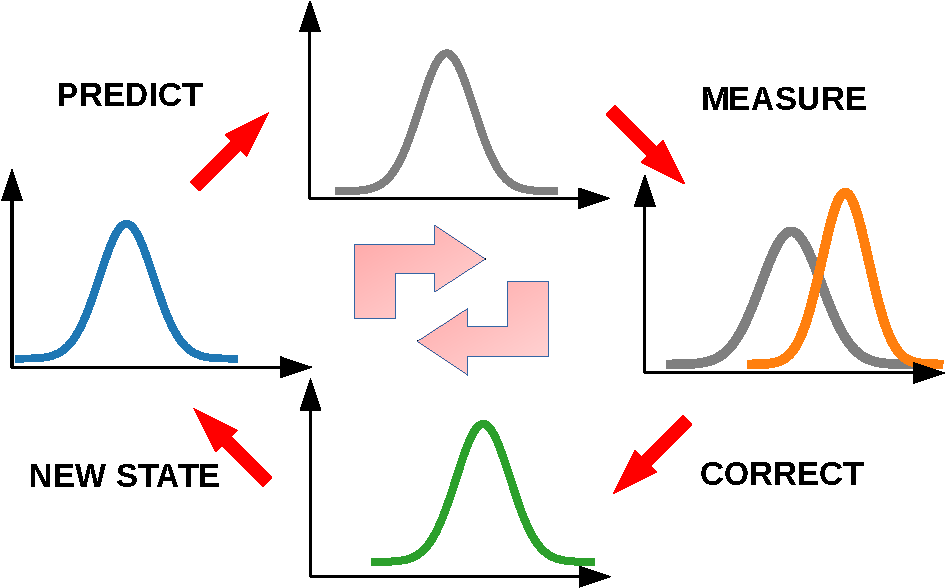
\includegraphics[width=0.7\linewidth]{figures/theoretical_foundations/kalman_filter_diagram.pdf}}
    \caption[A single iteration of the Kalman Filter]{Visualization of a single step of the Kalman Filter algorithm. Given some current state, the step begins with a prediction of the next state, then executing a measurement (in different literature a.k.a. making an observation), correcting the previous prediction in light of the newly gathered information, and in the end, using the updated variables as a basis for the next state in the future.}
    \label{fig:KalmanFilterDiagram}
\end{figure}

It is important to note that when dealing with object tracking, the Kalman Filter performs poorly in the presence of significant background clutter (spurious measurements not relating to any particular target). Clutter may introduce multimodal probability distributions over noise, which is tricky to cope with, given the already mentioned unimodal, Gaussian nature of the Kalman Filter. This realization led to the development of the Condensation (Conditional Density Propagation) algorithm, which detects and tracks objects contours in a cluttered environment~\cite{isard1998condensation}. However, this approach is outside of our scope, it just serves as a piece of evidence that sound predictions in the presence of noise are difficult to make with a linear model.

% ##################################################
\subsection{Particle Filter}
\label{ssec:ParticleFilter}

As~\cite{particle_filters_for_vot} states, particle filter has grown to be a standard tool for solving visual tracking problems in real-world applications. The particle Filter is meant to resolve many issues outlined above concerning the Kalman Filter, notably the lack of nonlinearity and the uni-modality of the probability distribution. We are not going to cover extensive mathematical details and derivations, but we will introduce the key concepts. Additionally, without loss of generality, we will primarily focus on object tracking applications. In a nutshell, this approach relies on a set of random samples with their associated weights that are then used to estimate the current state. The state can be anything, such as position, speed, size, etc. These samples together with weights are used to update the state and thus compute the new, approximated probability distribution~\cite{welch1995introduction}.

The particle filter is related to Bayesian algorithms in a way that it attempts to approximate an optimal Bayesian solution, since many relations in nonlinear Bayesian tracking are inherently intractable~\cite{Arulampalam2007}. Let us define the problem of tracking as an evolution of a state sequence $\cbrackets{\vect{x}_t \ | \ t \in \mathbb{N}}$, with $d_x$ being the dimension of the state vector $\vect{x}_t$. The state transition is governed by
\begin{equation}
    \label{eq:ProbModelStateEvolution}
    \vect{x}_t = \func{f_t}{\vect{x}_{t - 1}, \vect{v}_{t - 1}},
\end{equation}
where $\cbrackets{\vect{v}_t \ | \ t \in \mathbb{N}}$ is an i.i.d. process noise sequence of dimension $d_v$. The function $f_t$ may possibly be any nonlinear function of the state $\vect{x}_{t - 1}$ and represents a mapping $f_t = \mathbb{R}^{d_x} \times \mathbb{R}^{d_v} \to \mathbb{R}^{d_x}$~\cite{Arulampalam2007}. The objective is to estimate the state $x_t$ using recursion, provided that a sequence of measurements is available, concretely
\begin{equation}
    \vect{z}_t = \func{h_t}{\vect{x}_t, \vect{n}_t},
\end{equation}
where the function $h_t$ can be nonlinear, defining a mapping $h_t = \mathbb{R}^{d_x} \times \mathbb{R}^{d_n} \to \mathbb{R}^{d_z}$, such that $d_n$ and $d_z$ are dimensions of the measurement noise and measurement vectors, respectively. $\cbrackets{\vect{n}_t \ | \ t \in \mathbb{N}}$ is an i.i.d. measurement noise sequence. The aim is to produce estimates of $\vect{x}_t$ based on all the obtained measurements up to time $t$, denoted as $\vect{z}_{1:t} = \cbrackets{\vect{z_i} \ | \ i = 1, \dots, t}$~\cite{Arulampalam2007}.

The Bayes's Theorem plays an important role in estimating the probability $\probgiven{\vect{x}_t}{\vect{z}_{1:t}}$, the quantity recursively calculated up to some degree of belief. The assumption is that $\probgiven{\vect{x}_0}{\vect{z}_0} = \prob{\vect{x}_0}$ (a.k.a. the prior). Taking this into consideration, the $\probgiven{\vect{x}_t}{\vect{z}_{1:t}}$ may be acquired recursively, in two already introduced steps, \emph{prediction} and \emph{update}~\cite{Arulampalam2007}.

Assume that $\probgiven{\vect{x}_{t - 1}}{\vect{z}_{1:t - 1}}$ has already been computed. The prediction for the state $\vect{x}_t$ given all the previous measurements is then performed as
\begin{equation}
    \label{eq:BayesianOptimPrediction}
    \probgiven{\vect{x}_t}{\vect{z}_{1:t - 1}} = \int \probgiven{\vect{x}_t}{\vect{x}_{t - 1}} \probgiven{\vect{x}_{t - 1}}{\vect{z}_{1:t - 1}} d\vect{x}_{t - 1}.
\end{equation}
The equation~\ref{eq:BayesianOptimPrediction} exploits the Markov assumption which in this context states that $\probgiven{\vect{x}_t}{\vect{x}_{t - 1}, \vect{z}_{1:t - 1}} = \probgiven{\vect{x}_t}{\vect{x}_{t - 1}}$. The state evolution is defined in equation~\ref{eq:ProbModelStateEvolution}. At time step $t$, when a measurement $\vect{z}_t$ is obtained, the update stage follows to update the prior belief using the Bayes' rule
\begin{equation}
    \probgiven{\vect{x}_t}{\vect{z}_{1:t}} =
    \frac{
        \probgiven{\vect{z}_t}{\vect{x}_{t}}
        \probgiven{\vect{x}_t}{\vect{z}_{1:t - 1}}
    }{
        \probgiven{\vect{z}_t}{\vect{z}_{1:t - 1}}
    },
\end{equation}
where the normalizing constant in the denominator is
\begin{equation}
    \probgiven{\vect{z}_t}{\vect{z}_{1:t - 1}} =
    \int
    \probgiven{\vect{z}_t}{\vect{x}_{t}}
    \probgiven{\vect{x}_t}{\vect{z}_{1:t - 1}}
    d\vect{x}_t.
\end{equation}
It must be noted that this recursive propagation of the posterior density is only conceptual and is practically intractable. Nonetheless, there are restrictive cases where solutions do exists using for instance Kalman (section~\ref{ssec:KalmanFiler}) or particle Filter~\cite{Arulampalam2007}.

Particle Filter is a technique for implementing a recursive Bayesian filter outlined above through Monte Carlo simulations.  It is a powerful sequential state estimation approach~\cite{doucet2001introduction} based upon Monte Carlo integration techniques~\cite{mihaylova2007object}, so it is also known as the Sequential Monte Carlo algorithm. The core idea is to represent the posterior density function by a set of random samples with corresponding weights. Estimates are computed based on these samples and weights~\cite{Arulampalam2007}. A central characteristic of Monte Carlo simulations is that as the number of samples grows, the approximation also improves, approaching the optimal Bayesian estimate in the limit.

\cite{Arulampalam2007} further describes the algorithm, but we will finish off this section with a formalization of the density function approximation. Let $n_s$ be the number of support points that we will use to estimate the density function. Thus, let $\supsub{\cbrackets{\supsub{\vect{x}}{0:t}{i}, \supsub{w}{t}{i}}}{i = 1}{n_s}$ denote a \emph{random measure} characterizing the posterior probability density function $\probgiven{\vect{x}_{0:t}}{\vect{z}_{1:t}}$. The set $\cbrackets{\supsub{\vect{x}}{0:t}{i} \ | \ i = 0, \dots, n_s}$ contains the chosen support points. Each support point has an associated weight, and these quantities are represented by the set $\cbrackets{\supsub{w}{t}{i} \ | \ i = 1, \dots, n_s}$. When it comes to choosing the weights, the principle of \emph{importance sampling} (discussed later) is adhered to~\cite{bergman1999recursive, stordal2008sequential}. The set $\vect{x}_{0:t} = \cbrackets{\vect{x}_j \ | \ j = 0, \dots, t}$ stores all the state up to the specific time $t$. In addition, weights are normalized, satisfying the condition $\sum_{i = 1}^{n_s} \supsub{w}{t}{i} = 1$. In conformity with these definitions, the approximation of the posterior density at a given time $t$ is achieved by a discrete weighted approximation to the true posterior density function as follows:
\begin{equation}
    \probgiven{\vect{x}_{0:t}}{\vect{z}_{1:t}} \approx \sum_{i = 1}^{n_s} \supsub{w}{t}{i} \times \func{\delta}{\vect{x}_{0:t} - \supsub{\vect{x}}{0:t}{i}}.
\end{equation}

Since weights play an important role, and the whole process is an approximation, the exploitation of the \emph{importance sampling} method allows us to sample the weights from a probability distribution from which it is easy to obtain samples. However, this distribution should approximate the true distribution we would like to sample from, but are unable to. Let $\prob{x} \propto \func{\pi}{x}$ be the probability which it is complicated to obtain samples from, but evaluation of $\func{\pi}{x}$ is possible. Let $x^i \sim \func{g}{x}, i = 1, \dots, n_s$ portray easily generated samples according to some \emph{importance density} $\func{g}{\cdot}$. The weighted approximation is then
\begin{equation}
    \prob{x} \approx \sum_{i = 1}^{n_s} w^i \times \func{\delta}{x - x^i},
\end{equation}
with weights for each particle normalized according to
\begin{equation}
    w^i \propto \frac{\func{\pi}{x^i}}{\func{q}{x^i}}.
\end{equation}

Further description of derivation of all the equations introduced above, but using our newly established nomenclature according to importance sampling, will be omitted for the sake of clarity. More information can be found in~\cite{Arulampalam2007}.

% ##################################################
\subsection{Optical Flow}
\label{ssec:OpticalFlow}

The notion of optical flow is relevant to understand the motion of objects in the image between two consecutive frames, either caused by the movement of the object or camera itself. The combination of both is also possible, but it poses an additional complexity we will not deal with within our work. It describes a pattern of apparent motion. This description comes in the form of a $2D$ vector field, where each vector represents a displacement indicating the movement of points between first (previous) and the second (current) frame. Points of interest may be specially selected features (sparse optical flow, e.g. Lucas-Kanade method~\cite{Lucas1981}), or all the pixels of the image (dense optical flow, e.g. Gunnar-Farneback method~\cite{GunnarFarneback}). Deep learning has also been successfully applied using \glspl{cnn} for optical flow estimation, as demonstrated in~\cite{Dosovitskiy2015}.

Optical flow has been shown to enhance tracking performance~\cite{Leal-Taixe2016}, because it made possible to shrink the search region for localization of the \gls{bbox} of the object currently being tracked. In our work, we plan to ponder about the possibility to adopt such algorithms. The evidence suggests it may serve the purpose of supplementary information, similar to how a physical model of motion may complement visual tracking.

\begin{figure}[t]
    \centerline{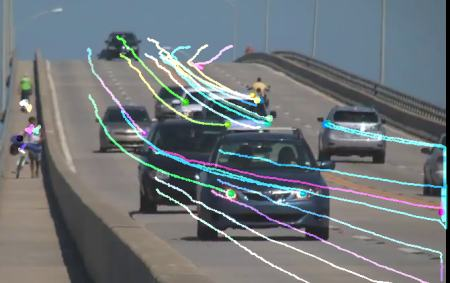
\includegraphics[width=0.5\linewidth]{figures/theoretical_foundations/opticalflow_lk.jpg}}
    \caption[Sparse optical flow]{An illustration of a sparse optical flow computed by the Lucas-Kanade algorithm~\cite{Lucas1981} across multiple frames. The drawn lines represent a trajectory of specifically selected features. Computation of the sparse optical flow also requires specific features to track. Those features can be determined by a plethora of algorithms, and one such a candidate is the handily named \emph{good features to track}~\cite{Shi1994} algorithm. \externalsrc{\cite{opticalflowimage}}}
    \label{fig:OpticalFlowLucasKanade}
\end{figure}

When estimating the optical flow, time starts to play a role. Besides, there are two assumptions upon which these algorithms operate:
\begin{enumerate}
    \item there is no change in pixel intensity between the two consecutive frames,
    \item motion is similar in neighboring pixels.
\end{enumerate}
Thus, let $\func{I}{x, y, t}$ be the coordinates of some pixel in the considered image. Assume this pixel moves by a distance $\Delta x$ and $\Delta y$ in $x$ and $y$ direction, respectively. Let $\Delta t$ stand for the time the movement took between the previous and current frame. Given the assumptions above, we have the relation
\begin{equation}
    \func{I}{x, y, t} = \func{I}{x + \Delta x, y + \Delta y, t + \Delta t}.
\end{equation}
Taking the Taylor expansion of the right-hand side produces the equation
\begin{equation}
    \frac{\partial I}{\partial x} \Delta x +
    \frac{\partial I}{\partial y} \Delta y +
    \frac{\partial I}{\partial t} \Delta t =
    0,
\end{equation}
where division by the $\Delta t$ term yields
\begin{equation}
    \frac{\partial I}{\partial x} \frac{\Delta x}{\Delta t} +
    \frac{\partial I}{\partial y} \frac{\Delta y}{\Delta t} +
    \frac{\partial I}{\partial t} = 0,
\end{equation}
and after substitution
\begin{equation}
    \label{eq:OpticalFlowEquation}
    \frac{\partial I}{\partial x} \nu_x +
    \frac{\partial I}{\partial y} \nu_y +
    \frac{\partial I}{\partial t} =
    0.
\end{equation}

Gradients of the image with respect to $x$, $y$ and $t$, represented by $\frac{\partial I}{\partial x}$, $\frac{\partial I}{\partial y}$ and $\frac{\partial I}{\partial t}$, can be easily obtained. However, there are two unknowns, namely $\nu_x$ and $\nu_y$ (main components of the velocity, or the optical flow of the image $\func{I}{x, y, t}$) the values of which cannot be solved because only one equation is available. To this end, various methods have been proposed, and equation~\ref{eq:OpticalFlowEquation} is appropriately called the \emph{optical flow equation}~\cite{fleet2006optical}.

\section{Visual Object Tracking}
\label{sec:VisualObjectTracking}

In this section, we will focus on the \emph{main topic} of this thesis: \textbf{tracking objects visually}. For simplicity, we will first introduce works within the single object tracking category. Section~\ref{sec:MultiObjectTracking} will continue with multiple object tracking.

Many research activities have been devoted to dealing with tracking of objects where visual input is the only information a model is provided with. Since the field of computer vision as a whole has transitioned from manual feature engineering in combination with shallow machine learning algorithms to using deep neural networks in end-to-end style, \gls{vot} as a subfield is no exception. We are going to discuss primarily \gls{sota} approaches, and if we do mention older, maybe even obsolete methods, it will be only for the sake of reference and historical motivation. Furthermore, unless stated otherwise, we will assume a general object tracking model.

\subsection{Initial Deep Learning-Based Solutions}
\label{ssec:InitialDeepLearningBasedSolutions}

At a time of publishing~\cite{held2016goturn}, most generic object trackers required online training from scratch, without taking advantage of available datasets to at least provide a starting point by initial offline training. This was the incentive behind development of the famous \gls{goturn}~\cite{held2016goturn}. This approach used to be \gls{sota} in single object tracking, but nowadays it is considered obsolete. A major issue is that the object has to be located initially, and occlusion handling is not performed as well as management of abrupt changes in position. So it is common for the object to drift away. Nevertheless, it stands to reason that the notion of leveraging data for offline training has pervaded the \gls{vot} community ever since. Nowadays, it is scarce to find a tracker that is trained online purely from scratch.

Given an initial state in a form of a \gls{bbox} belonging to the first frame (a search region), the network then crops a new region in the next frame and tries to find the location of the target object within this region. It practically performs a comparison of the current search region given the predicted target location from the previous frame. The previous frame is cropped and scaled so that it is centered on the target object. A small padding is made to allow for contextual information (see \figstr{}~\ref{fig:GOTURNFramework}). A key concept to highlight is that \gls{goturn} addresses the tracking as a box regression problem. In contrast, as will be presented later, similarity learning performs even better (section~\ref{ssec:TrackingUsingSiameseNetworks}).

\begin{figure}[t]
    \centerline{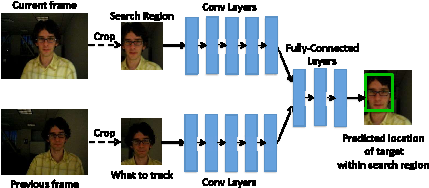
\includegraphics[width=0.8\linewidth]{figures/theoretical_foundations/goturn_framework.pdf}}
    \caption[\Gls{goturn} architecture]{The architecture of \gls{goturn} showing the input as a search region from the current frame where the target from the previous frame is to be searched for. The network essentially learns to localize the target within the cropped region. \externalsrc{\cite{held2016goturn}}}
    \label{fig:GOTURNFramework}
\end{figure}

\subsection{Fully Convolutional Tracking}
\label{ssec:FullyConvolutionalTracking}

We will start with a discussion about approaches that are so-called \emph{fully convolutional}. Transfer learning, e.g., exploiting an already pre-trained \gls{cnn} model to extract visual features, often comes with one drawback: the model accepts only a fixed input size. Although newer architectures can handle variable input size, this trait is more prevalent in object detection and segmentation than in basic task of image classification. A common approach is to resize the image to the required dimension, but this may significantly distort important features. Using fully connected layers demands known dimensions in advance, which is complicated to acquire when dealing with input of diverse shape. Convolutional layers are invariant to input size, therefore an avoidance of fully connected layers may provide an answer. An efficient solution to replace fully connected layers utilizes $1 \times 1$ convolutions notably propagated in \modelname{Network In Network} model~\cite{lin2014netinnet}. $1 \times 1$ filters were also used in the \modelname{Inception} architecture for dimensionality reduction and at the same time to increase the dimensionality of feature maps~\cite{szegedy2015inception}.

The \glspl{cnn} provide valuable spatial clues about the image content. As we touched upon in section~\ref{ssec:ConvolutionalNeuralNetworks}, convolutional layers placed at the bottom (beginning) of the model tend to capture elementary details useful for discriminating between targets of similar appearance, whilst top layers (at the end) seize more abstract information regarding separate object categories. Thus, interclass variations are thoroughly captured in the top layers, and intraclass variations conversely in the bottom layers (\figstr{}~\ref{fig:FullyCNNTrackingFeatureMaps}). This concept led the authors of~\cite{wang2015votcnn} to propose a fully convolutional visual object tracker that exploits different layers of the pre-trained VGG network~\cite{simonyan2015verydeepcnn} (\figstr{}~\ref{fig:FullyCNNTrackingSNetGNet}). Thus, the model responsible for extracting visual features is no longer treated as a black-box. An in-depth study was conducted on the properties of \gls{cnn} features of the offline pre-trained model for the task of classification of ImageNet dataset~\cite{deng2009imagenet}. It was found out, as suggested above, that characterization from different perspectives is provided by convolutional layers at different levels. Moreover, only a small subset of neurons is actually relevant for the tracking process itself. In connection with this, a feature map selection method was developed to aid in the removal of irrelevant (noisy) feature maps, with a consequence of reducing computational complexity while improving tracking accuracy.

The motivation for the utilization of different convolutional layers was that existing appearance-based tracking methods adopted either generative or discriminative models for separating the foreground from the background~\cite{wang2015votcnn}. To denote the distinction between the two, assume a classification task with the goal of estimating a function $f: X \to Y$, or $\probgiven{Y}{X}$, where $X$ represents the data and $Y$ the associated labels. A generative classifier would estimate parameters $\probgiven{X}{Y}$ and $\prob{Y}$ (in essence, the joint probability $\prob{X, Y}$) from the training data and then use the Bayes' rule to compute $\probgiven{Y}{X}$. On the other hand, a discriminative classifier would estimate parameters of $\probgiven{Y}{X}$ from the training data directly~\cite{ng2002discriminative}. The reliance of such foreground-background separation models on low-level hand-crafted features is considered a major drawback thanks to the incapability to capture semantic information and not being robust to appearance changes. The use features generated by \glspl{cnn} resolved much of such issues.

\begin{figure}[t]
    \centering
    \begin{subfigure}[b]{0.13\textwidth}
        \centering
        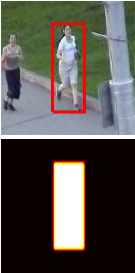
\includegraphics[width=\textwidth]{figures/theoretical_foundations/fully_cnn_tracking_feature_maps_1.pdf}
        \caption[]{}
    \end{subfigure}
    \hfill
    \begin{subfigure}[b]{0.39\textwidth}
        \centering
        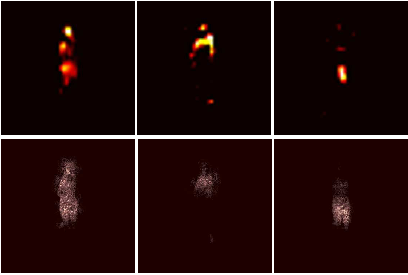
\includegraphics[width=\textwidth]{figures/theoretical_foundations/fully_cnn_tracking_feature_maps_2.pdf}
        \caption[]{}
    \end{subfigure}
    \hfill
    \begin{subfigure}[b]{0.39\textwidth}
        \centering
        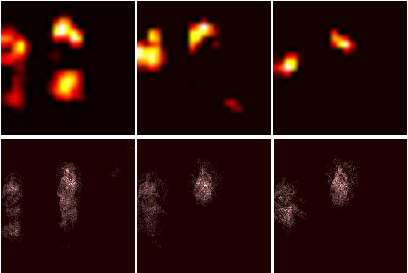
\includegraphics[width=\textwidth]{figures/theoretical_foundations/fully_cnn_tracking_feature_maps_3.pdf}
        \caption[]{}
    \end{subfigure}
    \caption[Fully convolutional tracking]{A \gls{cnn} model trained on image classification task carries spatial information. \imgpartdesc{a} Input image with an associated ground truth mask. \imgpartdesc{b} Visualization of feature maps from convolutional layers placed at the bottom of the model, capturing differences between foreground and background of a particular object instance. \imgpartdesc{c} As opposed to the previous group of images, a more holistic, abstract view on the object category itself is provided by feature maps from top convolutional layers. The top row in the \imgpartdesc{b} and \imgpartdesc{c} represents feature maps, whereas the bottom row represents the corresponding saliency map with spatial information of the category. \externalsrc{\cite{wang2015votcnn}}}
    \label{fig:FullyCNNTrackingFeatureMaps}
\end{figure}

Authors of~\cite{wang2015votcnn} put together a list of three observations that summarize properties of the fully convolutional nature of a tracker proposed by them.
\begin{itemize}
    \item Despite a large receptive field of \gls{cnn} feature maps, few of them are activated and they are sparsely distributed, localized, and correlated to the regions of semantic objects.
    \item The majority of the feature maps can be considered noisy or irrelevant when discriminating a specific target object (foreground) from the background.
    \item Different layers encode different types of features (related to the intraclass or interclass variations discussed at the beginning).
\end{itemize}
The proposed architecture in accordance to the aforementioned observation is described in \figstr{}~\ref{fig:FullyCNNTrackingFeatureMaps} and \figstr{}~\ref{fig:FullyCNNTrackingSNetGNet}.

\begin{figure}[t]
    \centerline{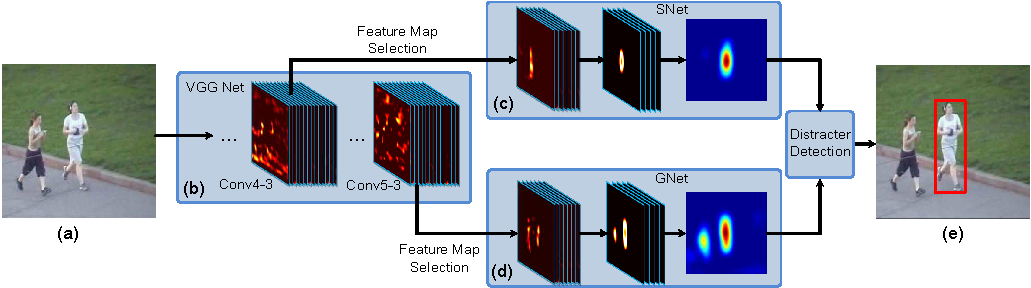
\includegraphics[width=\linewidth]{figures/theoretical_foundations/fully_cnn_tracking_snet_gnet.pdf}}
    \caption[Architecture of fully convolutional tracking]{For a given image, a feature map selection is performed on two different layers of the VGG network~\cite{simonyan2015verydeepcnn} to select the most relevant ones. This selection is handled as a heat map regression problem. A general network (GNet) captures the category information, whilst the specific network (SNet) captures visual traits based on which the foreground is separated from the background. Two heat maps are produced by these networks forming a basis for subsequent target localization. Both of these networks have to be initialized in the first frame. Afterward, when a new frame is to be processed, a region of interest is centered at the last target location, and the whole process repeats. \externalsrc{\cite{wang2015votcnn}}}
    \label{fig:FullyCNNTrackingSNetGNet}
\end{figure}

\subsection{Tracking Using Siamese Networks}
\label{ssec:TrackingUsingSiameseNetworks}

Even though \glspl{cnn} condense valuable visual information into low dimensional space upon which a tracker may be built, it is still not sufficient in many situations during object tracking. The object representation from convolutional layers trained on image classification is not robust enough for dramatic visual changes and occlusion of varying intensity. As we discussed in section~\ref{sec:LatentSpacesAndEmbeddings} dedicated to metric spaces and embeddings, an object representation supporting re-identification requires different types of models, one of which is a \emph{Siamese network} (section~\ref{ssec:SiameseAndTripletNetworks}). We have already mentioned our intention of utilizing custom metric space for tracking, and~\cite{bertinetto2016siamfc} were among the first ones to successfully demonstrate it.

Authors of~\cite{bertinetto2016siamfc} approved of the idea that visual feature extraction using \glspl{cnn} is pertinent to the robustness of the tracking algorithm, yet they advocated to train the visual model to a more general task of similarity learning rather than just classification. This observation and its further implementation was the main contribution of their work, achieving \gls{sota} performance back then. Broadly speaking, they trained a \emph{fully convolutional} Siamese network to locate an \emph{exemplar} image within a larger \emph{search} image (\figstr{}~\ref{fig:FullyCNNSiamTrackingArch}). The model got the name \modelname{Siam-FC}. We mentioned this to make the comparison easier because a lot of follow-up work has been done, producing models such as \modelname{SA-Siam}~\cite{he2018twofoldsiam}, \modelname{Siam-RPN}~\cite{li2018siamrpn}, \modelname{Siam-Mask}~\cite{wang2019siammask}, \modelname{Siam-Mask-E}~\cite{chen2019rotbboxes} and so forth.

Let $\gamma$ be a transformation that extracts visual features from the input, and $g$ be the function that combines two representations produced by the function $\gamma$. Siamese networks apply this identical transformation $\gamma$ to both inputs, search image $x$ and exemplar image $z$, and then combine the result as $\func{f}{x, z} = \func{g}{\func{\gamma}{x}, \func{\gamma}{z}}$. As such, when trivial distance or similarity measure is computed by the function $g$, then $\gamma$ can be deemed as the already introduced embedding.

\begin{figure}[t]
    \centerline{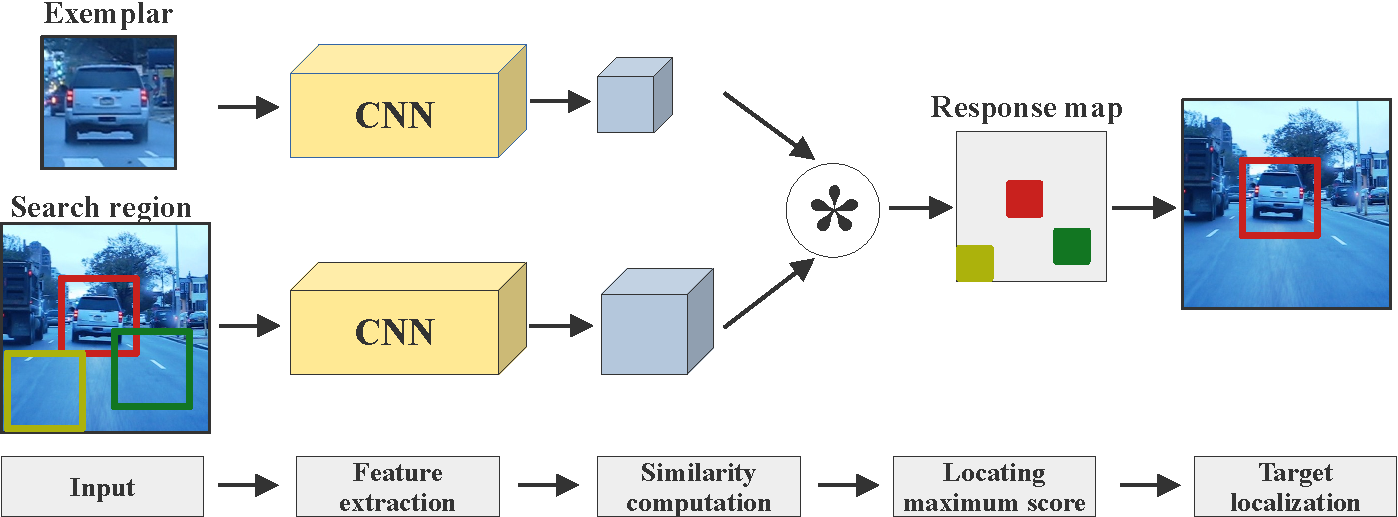
\includegraphics[width=0.7\linewidth]{figures/theoretical_foundations/fully_cnn_siam_tracking_architecture.pdf}}
    \caption[\modelname{Siam-FC} architecture]{The fully-convolutional Siamese architecture produces a scalar-valued score map, the size of which depends on the size of the search image. The similarity function is computed for all sub-windows within the search image and stored in a 2D score map, rather than just a pure 1D embedding vector. This computation requires only one evaluation. In this image, the red and blue pixels in the output score map represent similarity values for the two sub-windows on the input. Best viewed in color. \externalsrc{\cite{bertinetto2016siamfc}}}
    \label{fig:FullyCNNSiamTrackingArch}
\end{figure}

The use of the Siamese architecture spawned a lot of follow-up work, and we will describe some that serve our purposes. A team of authors in~\cite{he2018twofoldsiam} made the following observation: features learned in an image classification task (denoted as semantic features) complement features learned in a similarity matching task (denoted as appearance features). They also suitably commented that the key to designing a high-performance tracker is to harness expressive features that are simultaneously discriminative and generalized. In light of this, they developed a model consisting of a semantic and an appearance branch (see \figstr{}~\ref{fig:TwofoldSiameseNetArchitecture}), with each branch being represented by a standard similarity-learning Siamese network (as in \modelname{Siam-FC}~\cite{bertinetto2016siamfc}). However, an important distinction is that these two branches were trained separately, making them effectively heterogeneous to avoid any sharing of information. They reported that both branches were less powerful when trained jointly than when trained separately. The rationale behind such a decision was that each branch provides different features produced at different levels of abstraction, yet they complement each other. The merge of their respective outputs happens only during the testing time.

\begin{figure}[t]
    \centerline{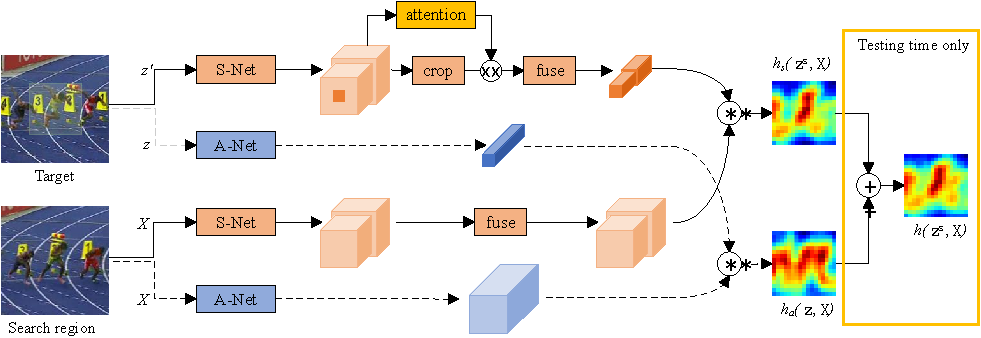
\includegraphics[width=\linewidth]{figures/theoretical_foundations/twofold_siamese_net_architecture.pdf}}
    \caption[\modelname{SA-Siam} architecture]{The architecture of the \modelname{SA-Siam} network. The \modelname{A-Net} represents the appearance network and the \modelname{S-Net} represents the semantic network. For the reason that this work builds on \modelname{Siam-FC} model~\cite{bertinetto2016siamfc}, structures connected by dotted lines are exactly the same as in the \modelname{Siam-FC} model. The last two convolutional layers provide features that are extracted afterward. The attention model determines the weight of each feature channel by simultaneous consideration of target and context information. The fusion module is trivial and uses just $1 \times 1$ convolutions. As shown on the right, combining branches is allowed only when testing. \externalsrc{\cite{he2018twofoldsiam}}}
    \label{fig:TwofoldSiameseNetArchitecture}
\end{figure}

The \modelname{SA-Siam} receives an input as a pair of image patches (\figstr{}~\ref{fig:TwofoldSiameseNetArchitecture}) cropped from the initial (target) frame and the current frame. Let $z$, $z^s$ and $X$ be the image of target, target including the surrounding context and the search region, respectively. Dimensions of $x^s$ and $X$ are identical, $W_s \times H_s \times 3$. Dimensions of the target $z$ located in the exact center of the region of $z^s$ are $W_t \times H_t \times 3$, such that $W_t < W_s$ and $H_t < H_s$. The appearance branch (\modelname{A-Net}) takes $\rbrackets{z, X}$ as input and essentially clones the entire \modelname{Siam-FC} network. Let $\func{f_a}{\cdot}$ denote the visual features extracted by the \modelname{A-Net}. Then, the response map of this branch is given by
\begin{equation}
    \func{h_a}{z, X} = \func{corr}{\func{f_a}{z}, \func{f_a}{X}},
\end{equation}
where $\func{corr}{\cdot}$ is the correlation operation. The training of this branch is rather straightforward thanks to the abundance of training pairs $\rbrackets{z_i, X_i}$ with their related response map $Y_i$, for $i = 1, \dots, N$, with $N$ being the no. of chosen training samples. The parameters $\theta_a$ of the \modelname{A-Net} model are optimized from scratch by minimizing the logistic loss function $\func{\mathcal{L}}{\cdot}$:
\begin{equation}
    \label{eq:ANetModelTraining}
    \underset{\theta_a}{\argmin}
    \frac{1}{N}
    \cbrackets{
        \func{\mathcal{L}}{
            \func{h_a}{z_i, X_i; \theta_a},
            Y_i
        }
    }.
\end{equation}

Analogically, the semantic branch (\modelname{S-Net}) assumes as input a pair $\rbrackets{z^s, X}$. Contrary to the \modelname{A-Net}, this model is pre-trained for the image classification task and its weights are frozen during the training phase. These last two convolutional layers of this model are of primary interest as their features provide abstraction at distinct levels. However, spatial resolutions are not alike. Let $\func{f_s}{\cdot}$ be the concatenated multilevel features. For the correlation operation ($\func{corr}{\cdot}$) to be usable, a special fusion module is introduced, implemented by a simple $1 \times 1$ convolution layer. The fusion operation is applied to features within the same layer, and this fused feature vector will be referred to as $\func{g}{\func{f_s}{X}}$.

Semantic features of higher-level are robust to appearance variation. This contributes to the generalization ability of the tracker but exacerbates its discriminative abilities. To circumvent this, the attention module is presented. The reasoning is that individual feature channels have varying importance for object tracking as far as different targets are concerned. The goal is then to assign a degree of importance (weight) to each channel for each target. Still, the target information is not sufficient, so the context must be supplied, too. The proposed attention module thus processes the feature map of $z^s$ instead of just $z$. Although the use of multilevel features in conjunction with the attention module delivers substantial progress for the semantic branch, it would be counterproductive for the appearance branch. Appearance features extracted from different convolutional layers lack sufficient differences in terms of expressiveness, as these features are dense whereas high-level semantic features are very sparse.

The attention module operates channel-wise. Assume the $i^{\text{th}}$ channel from some convolutional feature map with spatial dimensions of $22 \times 22$ is being processed. The tracking target is contained in the center, covering a region of $6 \times 6$. The entire feature map is divided into a grid of $3 \times 3$ cells. Within each grid, a max-pooling operation is applied followed by a simple neural network consisting of just $1$ hidden layer. The weight coefficient $\zeta_i$ for the particular $i^{\text{th}}$ channel is generated by the sigmoid activation function (\figstr{}~\ref{fig:TwofoldSiameseNetAttentionModule}). The attention module incurs negligible computational overhead as it's only active during the target processing on the first frame. Later on, the weight coefficient is used to scale each feature map according to its importance. The response map for the semantic branch is produced as
\begin{equation}
    \func{h_s}{z^s, X} =
    \func{corr}{
        \func{g}{\zeta \cdot \func{f_s}{z}},
        \func{g}{\func{f_s}{X}}
    },
\end{equation}
where the no. of elements of $\zeta$ is equal to the no. of channels in $\func{f_s}{z}$, and the operator $\cdot$ indicates an element-wise multiplication.

\begin{figure}[t]
    \centerline{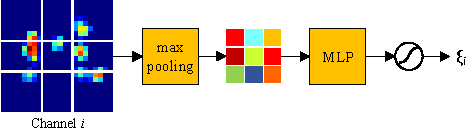
\includegraphics[width=0.6\linewidth]{figures/theoretical_foundations/twofold_siamese_net_attention_module.pdf}}
    \caption[\modelname{S-Net} attention module]{The attention module of the \modelname{S-Net} network. \externalsrc{\cite{he2018twofoldsiam}}}
    \label{fig:TwofoldSiameseNetAttentionModule}
\end{figure}

When training the \modelname{S-Net} branch, only the fusion and the attention modules are updated. No fine-tuning techniques are taken advantage of, regardless of the potential improvement of the semantic branch alone. Authors informed about such experiments, and they resulted in diminished overall performance thanks to \modelname{A-Net} and \modelname{S-Net} becoming less heterogeneous. Let $\rbrackets{\subsup{z}{i}{s}, X_i}$ with their corresponding ground-truth response map $Y_i$, for $i = 1, \dots, N$, be the $N$ chosen training samples. The parameters $\theta_s$ of the \modelname{S-Net} model are fitted using the logistic loss function $\func{\mathcal{L}}{\cdot}$ (equal to equation~\ref{eq:ANetModelTraining})
\begin{equation}
    \label{eq:SNetModelTraining}
    \underset{\theta_s}{\argmin}
    \frac{1}{N}
    \cbrackets{
        \func{\mathcal{L}}{
            \func{h_a}{\subsup{z}{i}{s}, X_i; \theta_a},
            Y_i
        }
    }.
\end{equation}
The inference phase involves computation of the overall heat map for which a weighted average of the two produced heat maps is used as shown below:
\begin{equation}
    \func{h}{z, z^s, X} = \lambda \func{h_a}{z, X} + \rbrackets{1 - \lambda} \func{h_s}{z^s, X}.
\end{equation}
This introduces another hyperparameter $\lambda$ (where $0 < \lambda < 1$) that can in practice be reliably estimated from the validation dataset.

The series of Siamese-based architectures for tracking continued with the idea of using the \gls{rpn}~\cite{li2018siamrpn} (see section~\ref{ssec:FasterRCNN} for the same concept applied in object detection). Under the flag of end-to-end training, the \modelname{SiamRPN} model consists of a Siamese subnetwork for feature extraction (again, a duplicate of the \modelname{SiamFC}~\cite{bertinetto2016siamfc}) and \gls{rpn} as another subnetwork encompassing both classification and regression branch (\figstr{}~\ref{fig:SiamRPNNetArchitecture}). The notable contribution is that the proposed framework is formulated as a local one-shot detection task in the inference phase (the first work to make such a step) (\figstr{}~\ref{fig:SiamRPNOneShotDetection}). The template branch encodes the object appearance information for further foreground/background discrimination. Analogically, the \gls{bbox} from the first frame is the only exemplar for one-shot detection in the inference phase.

The region proposal subnetwork contains a pair-wise correlation section as well as a supervision section. Let $k$ denote the number of anchors. Then, the model has to output $2k$ channels for the classification and $4k$ channels for the regression. Following the established notation, the Siamese subnetwork produces feature maps $\func{\gamma}{z}$ and $\func{\gamma}{x}$. The pair-wise correlation splits $\func{\gamma}{z}$ into $\sbrackets{\func{\gamma}{z}}_{cls}$ and $\sbrackets{\func{\gamma}{z}}_{reg}$ while increasing the no. of channels (\figstr{}~\ref{fig:SiamRPNNetArchitecture}). Conversely, $\func{\gamma}{x}$ is also split into $\sbrackets{\func{\gamma}{x}}_{cls}$ and $\sbrackets{\func{\gamma}{x}}_{reg}$, but the no. of channels remains unchanged. The correlation, when computed on both branches, is given by
\begin{equation}
    \begin{aligned}
        \subsup{A}{w \times h \times 2k}{cls} & =
        \sbrackets{\func{\gamma}{x}}_{cls} \star \sbrackets{\func{\gamma}{z}}_{cls}, \\
        \subsup{A}{w \times h \times 4k}{reg} & =
        \sbrackets{\func{\gamma}{x}}_{reg} \star \sbrackets{\func{\gamma}{z}}_{reg},
    \end{aligned}
\end{equation}
where the template feature maps $\sbrackets{\func{\gamma}{z}}_{cls}$ and $\sbrackets{\func{\gamma}{z}}_{reg}$ stand in place of kernels in the convolution operation signified by the $\star$ character.

\begin{figure}[t]
    \centerline{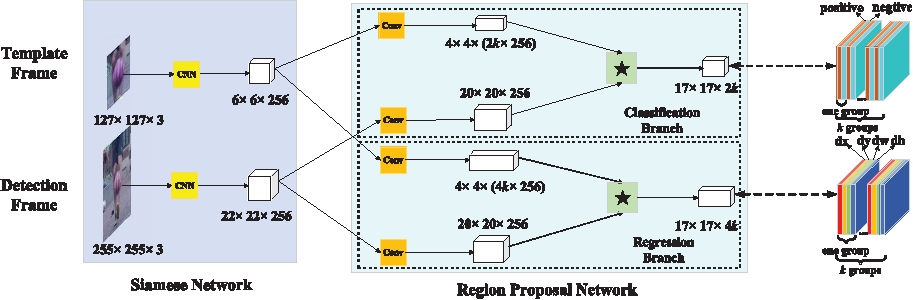
\includegraphics[width=\linewidth]{figures/theoretical_foundations/siam_rpn_architecture.pdf}}
    \caption[\modelname{Siam-RPN} architecture]{The pipeline starts with the original \modelname{Siam-FC} network followed by the \gls{rpn} which has two branches: classification and regression. The output of the two branches is obtained using a pair-wise correlation. Foreground/background classification and the box regression are given by the $17 \times 17 \times 2k$ and $17 \times 17 \times 4k$ feature maps, respectively. \externalsrc{\cite{li2018siamrpn}}}
    \label{fig:SiamRPNNetArchitecture}
\end{figure}

The noteworthy formulation of tracking as one-shot detection was proposed as follows. In general terms, the goal is to minimize the average loss $\mathcal{L}$ of a predictor function $\func{\psi}{x; W}$ by finding its parameters $W$. When computed over a dataset of $N$ samples $x_i$ with corresponding labels $y_i$, $\forall i = 1, \dots, N$, it is given by
\begin{equation}
    \label{eq:SiamRPNOneShotGeneral}
    \underset{W}{\argmin}
    \cbrackets{
        \frac{1}{N}
        \sum_{i = 1}^{N}
        \func{\mathcal{L}}{
            \func{\psi}{x_i; W},
            y_i
        }
    }.
\end{equation}
\emph{One-shot learning} aims to learn $W$ when only a single template $z$ is available.
Discriminative one-shot learning tackles a major challenge of \emph{learning to learn}, by finding a mechanism to integrate category information into the learner~\cite{bertinetto2016oneshot}. If we consider a meta-learning feed-forward function $\omega$ that maps $\rbrackets{z_i; W'}$ to $W$, then the problem can be stated as
\begin{equation}
    \label{eq:SiamRPNOneShotMetaLearning}
    \underset{W'}{\argmin}
    \cbrackets{
        \frac{1}{N}
        \sum_{i = 1}^{N}
        \func{\mathcal{L}}{
            \func{\psi}{x_i; \func{\omega}{z_i, W'}},
            y_i
        }
    }.
\end{equation}
In this setting, this objective function can be re-written in terms of the Siamese subnetwork feature extraction $\gamma$ and region proposal subnetwork $\Psi$ as
\begin{equation}
    \label{eq:SiamRPNOneShoCombo}
    \underset{W}{\argmin}
    \cbrackets{
        \frac{1}{N}
        \sum_{i = 1}^{N}
        \func{\mathcal{L}}{
            \func{\Psi}{\func{\gamma}{x_i; W}; \func{\gamma}{z_i; W}},
            y_i
        }
    }.
\end{equation}
The template branch provides training parameters to predict the kernel for the detection task, a typical example of the \emph{learning to learn} process. The template branch, therefore, embeds necessary category information into the kernel that is subsequently utilized for detection (\figstr{}~\ref{fig:SiamRPNOneShotDetection}). The last thing to consider is how to propose and then select the regions. One strategy is to discard boxes too far away from the object's center. A possible implementation is to keep $g \times g$ subregion of the $\subsup{A}{w \times h \times 2k}{cls}$ feature map resulting in $g \times g \times k$ anchors instead of $w \times h \times k$. This idea is the beginning of a further refined notion in future papers of the so-called \emph{centerness} that plays an important role in weighting \glspl{bbox}. Another strategy would be to use a cosine window to help in computing a penalty bound to a too large displacement in size and ratio. Afterwards, the \gls{nms} (section~\ref{ssec:NonMaximumSuppression}) is applied to get the final tracking \gls{bbox}.

\begin{figure}[t]
    \centerline{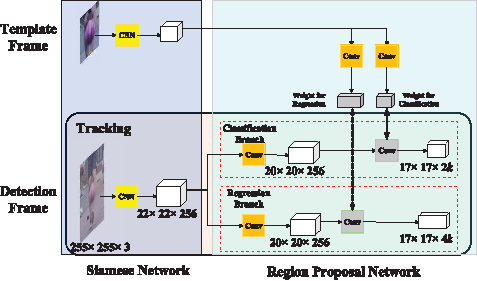
\includegraphics[width=0.7\linewidth]{figures/theoretical_foundations/siam_rpn_one_shot_detection.pdf}}
    \caption[Tracking as one-shot detection]{Tracking is framed as one-shot detection here. First, the template branch predicts the weights of the kernels for the \gls{rpn} using the first frame. Later on, only the detection branch is retained so the framework can be thought of as a local detection network. \externalsrc{\cite{li2018siamrpn}}}
    \label{fig:SiamRPNOneShotDetection}
\end{figure}

Later on, a fork of publications emerged with an endeavor to improve the tracking performance by estimating not only a regular axis-aligned \gls{bbox}, but a rotated box, too. Put into perspective, the rotated \gls{bbox}, as opposed to an ordinary, axis-aligned, contains the minimal amount of background pixels~\cite{chen2019rotbboxes}. Thus, datasets with rotated \glspl{bbox} provide tighter enclosed boxes. Additionally, the orientation information may be useful for solving different computer vision problems, such as action classification.

Inspiration from techniques for the problem of object segmentation yielded another approach where the tracking process was assisted with additional semi-supervised object segmentation~\cite{wang2019siammask}. The relevant contribution is the augmentation of the training loss with a binary segmentation task. Further, once trained, the model (dubbed \modelname{Siam-MASK}) relies exclusively upon a single \gls{bbox} initialization and operates online while producing rotated \glspl{bbox} instead of axis-aligned ones together with class-agnostic object segmentation masks. Notwithstanding its convenience, a single rectangle frequently fails to represent the object appropriately, hence the motivation to generate additional segmentation masks.

As always, the \modelname{SiamFC}~\cite{bertinetto2016siamfc} was employed as the fundamental building block. However, a notable alternation consisted of the use of a depth-wise cross-correlation layer instead of a simple cross-correlation layer. The latter one compresses all the information into one channel, impeding the potential to encode richer information about the target object. As a reminder, the original model used $6 \times 6 \times 128$ and $22 \times 22 \times 128$ tensors to produce a $17 \times 17 \times 1$ response map (\figstr{}~\ref{fig:FullyCNNSiamTrackingArch}). Here, a multi-channel response maps are utilized (\figstr{}~\ref{fig:SiamMaskArchitecture}).

\begin{figure}[t]
    \centering
    \begin{subfigure}[b]{0.68\textwidth}
        \centering
        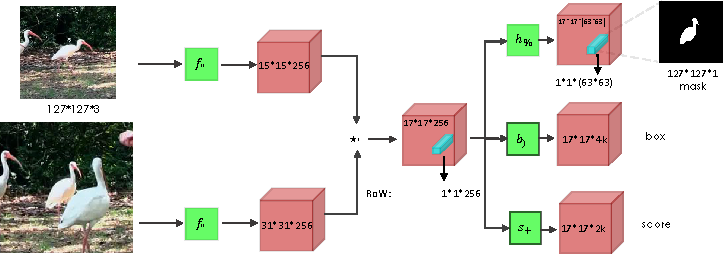
\includegraphics[width=\textwidth]{figures/theoretical_foundations/siam_mask_architecture_3_branch.pdf}
        \caption[]{}
    \end{subfigure}
    \hfill
    \begin{subfigure}[b]{0.31\textwidth}
        \centering
        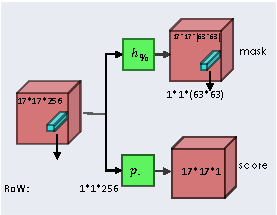
\includegraphics[width=\textwidth]{figures/theoretical_foundations/siam_mask_architecture_2_branch_head.pdf}
        \caption[]{}
    \end{subfigure}
    \caption[\modelname{Siam-Mask} architecture]{A schematic illustration of the two \modelname{Siam-Mask} variants: \imgpartdesc{a} a three-branch architecture (full), \imgpartdesc{b} a two-branch architecture (head). Depth-wise correlation layers are adopted again. \externalsrc{\cite{wang2019siammask}}}
    \label{fig:SiamMaskArchitecture}
\end{figure}

Let $z$ and $x$ be the exemplar and the search image, respectively. Then, these two inputs are processed by the same \gls{cnn} $f_\theta$ to yield $g_\theta$ using the cross-correlation as follows:
\begin{equation}
    \label{eq:SiamMaskCrossCorrelation}
    \func{g_\theta}{z, x} = \func{f_\theta}{z} \star \func{f_\theta}{x}.
\end{equation}
Authors contrived the term \gls{row} to represent each spatial element of the response map given by the left hand side of equation~\ref{eq:SiamMaskCrossCorrelation}. In that regard, the similarity between the exemplar $z$ and the $n$-th candidate window in $x$ is declared as $\func{\subsup{g}{\theta}{n}}{z, x}$. Throughout the training phase, $w \times h$ binary masks (one for each \gls{row}) using a trivial two-layer neural network $h_\phi$ are predicted. Let $\mtx{M_n}$ be the predicted segmentation mask corresponding to the $n$-th \gls{row},
\begin{equation}
    \mtx{M_n} = \func{h_\phi}{\func{\subsup{g}{\theta}{n}}{z, x}}.
\end{equation}
A ground-truth binary label $y_n \in \cbrackets{\pm 1}$ is assigned to each \gls{row} as well as pixel-wise ground-trith mask $\mtx{C_n}$ with dimensions $w \times h$. Let $\mtx{C}_n^{i,j} \in \cbrackets{\pm 1}$ denote the label corresponding to pixel at position $\rbrackets{i, j}$ within the segmentation mask in the $n$-th \gls{row}. The mask prediction task is driven by the binary logistic regression loss function $\mathcal{L}_{mask}$ over all \glspl{row}:
\begin{equation}
    \func{\mathcal{L}_{mask}}{\theta, \phi} =
    \sum_n
    \rbrackets{
    \frac{1 + y_n}{2wh}
    \sum_{i}
    \sum_{j}
    \func{\log}{1 + e^{-\mtx{C}_n^{i,j} \mtx{M}_n^{i,j}}}
    }.
\end{equation}

An incremental improvement of \modelname{Siam-Mask} model came when~\cite{chen2019rotbboxes} proposed a novel, efficient algorithm for the estimation of the \gls{bbox} rotation when the object segmentation mask is given. Particularly, a mask produced by the \modelname{Siam-Mask} model, as this work builds on top of~\cite{wang2019siammask}, under the derived name \modelname{Siam-Mask-E}. In addition, their approach can be used to generate a rotated box ground truth from any segmentation datasets to train a rotation angle regression model.

To estimate the rotation angle, they adopted the least-squared scheme as part of the ellipse fitting algorithm. Considering the standard conic equation
\begin{equation}
    ax^2 + bxy + cy^2 + dx + ey + f = 0,
\end{equation}
the ellipse can be formulated by adding a constraint
\begin{equation}
    b^2 - 4ac < 0,
\end{equation}
where $a$, $b$, $c$, $d$, $e$, and $f$ are the coefficients of the ellipse and $x$, $y$ represent any point on the ellipse. Let $\vectt{a}{a, b, c, d, e, f}$ and $\vectt{x}{x^2, xy, y^2, x, y, 1}$. The ellipse equation can then be written as
\begin{equation}
    \func{F}{\vect{x}} = \vect{x}^T\vect{a} = 0.
\end{equation}
Assume a dataset of $N$ points, $\mset{A} = \cbrackets{\rbrackets{x_1, y_1}, \rbrackets{x_2, y_2}, \dots, \rbrackets{x_N, y_N}}$, and a task of fitting an ellipse to the dataset $\mset{A}$. The goal is to find the coefficients of the vector $\vect{a}$, as determined by the objective function
\begin{equation}
    \underset{\vect{a}}{\argmin} \sum_{i = 1}^{N} {\func{F}{\vect{x}_i}}^2,
\end{equation}

\begin{figure}[t]
    \centerline{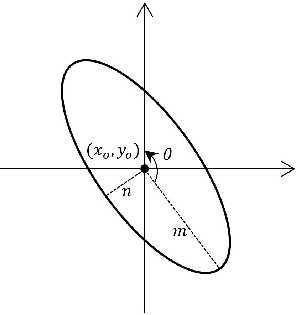
\includegraphics[width=0.4\linewidth]{figures/theoretical_foundations/fast_vot_rot_bbox_ellipse.pdf}}
    \caption[Ellipse notation]{Ellipse notation: $\rbrackets{x_0, y_0}$ is the center point around which the ellipse with semi-major axis $m$ and semi-minor axis $n$ is rotated by the angle $\theta$ in counter-clockwise direction. \externalsrc{\cite{chen2019rotbboxes}}}
    \label{fig:FastVOTRotBBOXEllipse}
\end{figure}
where $\vect{x}^T = \sbrackets{\subsup{x}{i}{2}, x_i y_i, \subsup{y}{i}{2}, x_i, y_i, 1}$ and $\mset{A}_i = \rbrackets{x_i, y_i}$.

For the upcoming description, we advise to follow the description for \figstr{}~\ref{fig:FastVOTRotBBOXFitting}. Once the coefficients are estimated, the rotation angle $\theta$ around the center point $\rbrackets{x_0, y_0}$ with semi-major $m$ and semi-minor axis $n$ are trivial to obtain (\figstr{}~\ref{fig:FastVOTRotBBOXEllipse}). The 2D affine transformation matrix
\begin{equation}
    \mtx{T} =
    \begin{bmatrix}
        \func{\cos}{\theta} &
        \func{\sin}{\theta} &
        \rbrackets{1 - \func{\cos}{\theta}}x_0 - \func{\sin}{\theta} y_0 \\
        -\func{sin}{\theta} &
        \func{\cos}{\theta} &
        \func{\sin}{\theta} x_0 - \rbrackets{1 - \func{\cos}{\theta}} y_0
    \end{bmatrix}
\end{equation}
is thereafter used to produce the set $\mset{M'}$, which contains the transformed (rotated and translated) points belonging to the input segmentation mask, denoted by the set $\mset{M}$, as
\begin{equation}
    \mset{M'} =
    \cbrackets{
        \mtx{T}
        \sbrackets{x, y, 1}^T
        \ | \
        \forall \rbrackets{x, y} \in \mset{M}
    }.
\end{equation}
Computing the \gls{bbox} $\vect{G}$ into which the ellipse after being transformed by $\mtx{T}$ is inscribed is rather straightforward:
\begin{equation}
    \vectt{G}{x_0 - n, y_0 - m, x_0 + n, y_0 + m}.
\end{equation}
Considering the extreme values for coordinates $x$ and $y$ below:
\begin{equation}
    \begin{aligned}
         & x_{min} = \min \cbrackets{x\ |\ \forall x \in \mset{M'}},
        \quad
         & x_{max} = \max \cbrackets{x\ |\ \forall x \in \mset{M'}}, \\
         & y_{min} = \min \cbrackets{y\ |\ \forall y \in \mset{M'}},
        \quad
         & y_{max} = \max \cbrackets{y\ |\ \forall y \in \mset{M'}},
    \end{aligned}
\end{equation}
then the the min-max axis-aligned \gls{bbox} $\vect{B}$ is given by
\begin{equation}
    \vectt{B}{x_{min}, y_{min}, x_{max}, y_{max}}.
\end{equation}
Combining $\vect{G}$ and $\vect{B}$ we have the intersection \gls{bbox} $\vect{R}$ calculated using the following equation:
\begin{equation}
    \vectt{R}{
        \max \cbrackets{\vect{G_1}, \vect{B_1}},
        \max \cbrackets{\vect{G_2}, \vect{B_2}},
        \min \cbrackets{\vect{G_3}, \vect{B_3}},
        \min \cbrackets{\vect{G_4}, \vect{B_4}}
    }.
\end{equation}
Let $\mset{R}$ be the set containing vertices of the box $\vect{R}$, thus
\begin{equation}
    \mset{R} = \cbrackets{
        \rbrackets{\vect{R_1}, \vect{R_2}},
        \rbrackets{\vect{R_3}, \vect{R_2}},
        \rbrackets{\vect{R_3}, \vect{R_4}},
        \rbrackets{\vect{R_1}, \vect{R_4}}
    }.
\end{equation}
The last step, the conversion of the transformed coordinates back to the original image coordinates, is performed using the inverse affine transformation matrix $\mtx{T}^{-1}$. The result of this operation is accomplished by
\begin{equation}
    \mset{R'} =
    \cbrackets{
        \mtx{T}^{-1}
        \sbrackets{x, y, 1}^T
        \ | \
        \forall \rbrackets{x, y} \in \mset{R}
    }.
\end{equation}

\begin{figure}[t]
    \centering
    \begin{subfigure}[b]{0.135\textwidth}
        \centering
        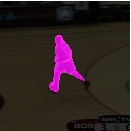
\includegraphics[width=\textwidth]{figures/theoretical_foundations/fast_vot_rot_bbox_algo_01.pdf}
        \caption[]{}
    \end{subfigure}
    \hfill
    \begin{subfigure}[b]{0.135\textwidth}
        \centering
        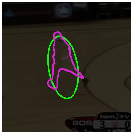
\includegraphics[width=\textwidth]{figures/theoretical_foundations/fast_vot_rot_bbox_algo_02.pdf}
        \caption[]{}
    \end{subfigure}
    \hfill
    \begin{subfigure}[b]{0.135\textwidth}
        \centering
        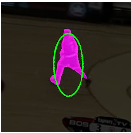
\includegraphics[width=\textwidth]{figures/theoretical_foundations/fast_vot_rot_bbox_algo_03.pdf}
        \caption[]{}
    \end{subfigure}
    \hfill
    \begin{subfigure}[b]{0.135\textwidth}
        \centering
        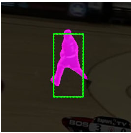
\includegraphics[width=\textwidth]{figures/theoretical_foundations/fast_vot_rot_bbox_algo_04.pdf}
        \caption[]{}
    \end{subfigure}
    \hfill
    \begin{subfigure}[b]{0.135\textwidth}
        \centering
        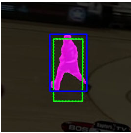
\includegraphics[width=\textwidth]{figures/theoretical_foundations/fast_vot_rot_bbox_algo_05.pdf}
        \caption[]{}
    \end{subfigure}
    \hfill
    \begin{subfigure}[b]{0.135\textwidth}
        \centering
        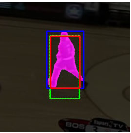
\includegraphics[width=\textwidth]{figures/theoretical_foundations/fast_vot_rot_bbox_algo_06.pdf}
        \caption[]{}
    \end{subfigure}
    \hfill
    \begin{subfigure}[b]{0.135\textwidth}
        \centering
        \includegraphics[width=\textwidth]{figures/theoretical_foundations/fast_vot_rot_bbox_algo_07.pdf}
        \caption[]{}
    \end{subfigure}
    \caption[Rotated \gls{bbox} by ellipse fitting]{\imgpartdesc{a} Edge pixels of the input segmentation mask, \imgpartdesc{b} ellipse fitting, \imgpartdesc{c} the affine transformation is computed and the points belonging to the mask are rotated and translated, \imgpartdesc{d} the ellipse is then inscribed into a rectangular box, \imgpartdesc{e} this box is then intersected with the min-max rectangular box, \imgpartdesc{f} the intersection box, \imgpartdesc{g} inverse affine transformation. \externalsrc{\cite{chen2019rotbboxes}}}
    \label{fig:FastVOTRotBBOXFitting}
\end{figure}

The idea to employ fully convolutional networks seems to pertain to the modern computer vision community. Besides a simpler model, the fully convolutional design often leads to a reduced number of hyperparameters. One such an architecture (a descendant of the famous \modelname{Siam-FC}~\cite{bertinetto2016siamfc} model) has been recently proposed, named \modelname{Siam-CAR}~\cite{guo2019siamcar}. This approach relies on the decomposition of the task of \gls{vot} into two subproblems: classification for pixel category and regression for object \gls{bbox} at the given pixel. The leading concept of the article is that this tracker operates in an end-to-end, per-pixel manner. The authors managed to avoid the use of anchors as well as region proposals, hence reducing the need for human intervention. The use of the two aforementioned traits commonly leads to sensitivity to dimensions and aspect ratios of the anchor boxes, which requires expertise on hyperparameter tuning for successful tracking.

\begin{figure}[t]
    \centerline{\includegraphics[width=\linewidth]{figures/theoretical_foundations/siamcar_architecture.pdf}}
    \caption[\modelname{Siam-CAR} architecture]{\modelname{Siam-CAR} architecture. The left side consists of the original \modelname{Siam-FC}~\cite{bertinetto2016siamfc} model, with a simple amendment of using depth-wise correlation for multi-channel response map extraction. The right side depicts the subnetworks for foreground/background classification and \gls{bbox} regression. \externalsrc{\cite{guo2019siamcar}}}
    \label{fig:SiamCARArchitecture}
\end{figure}

Let $R$ be the response map produced by a depth-wise correlation between the features extracted by the Siamese network from the exemplar $Z$ and the target $X$ (\figstr{}~\ref{fig:SiamCARArchitecture}). Then,
\begin{equation}
    R = \func{\gamma}{X} \star \func{\gamma}{Z}.
\end{equation}
An indispensable part of localization are low-level features like edges, corners, and so on, whereas high-level features strengthen the representational power from the semantic point of view, which is crucial for discrimination. Authors fused low-level and high-level features from the last $3$ residual blocks of the \modelname{ResNet-50} backbone (indicated by the $\func{F_3}{X}$, $\func{F_4}{X}$ and $\func{F_5}{X}$), forming a unity after concatenation (in case of $X$):
\begin{equation}
    \func{\gamma}{X} = \func{cat}{\func{F_3}{X}, \func{F_4}{X}, \func{F_5}{X}}.
\end{equation}
The resulting $\func{\gamma}{X}$ contains $3 \times 255$ channels since all $\func{F_i}{X}, \forall i = 3, 4, 5$, include $256$ channels. The response map $R$ is then convoluted with $1 \times 1$ kernel to reduce its dimension to $256$ channels, giving the reduced response map $R^*$.

At a later stage, the response map $\subsup{R}{w \times h \times m}{*}$ extracted by the Siamese subnetwork serves for classification and regression branches, producing feature maps $\subsup{A}{w \times h \times 2}{cls}$ and $\subsup{A}{w \times h \times 4}{reg}$, respectively. Each point $\rbrackets{i, j, :}$ in $\subsup{A}{w \times h \times 2}{cls}$ contains a $2D$ vector representing the foreground and background scores. Analogically, each point $\rbrackets{i, j, :}$ in $\subsup{A}{w \times h \times 4}{reg}$ contains a $4D$ vector $\vectt{t_{i, j}}{l, t, r, b}$ specifying distance from the corresponding location to the $4$ sides of the \gls{bbox} in the input search region. Let $\rbrackets{x_0, y_0}$ and $\rbrackets{x_1, y_1}$ denote the top-left and bottom-right corners of the ground-truth \gls{bbox} and $\rbrackets{x, y}$ the corresponding location of a point $\rbrackets{i, j}$. The regression target $\vect{\tilde{t}_{i, j}}$ at $\subsup{A}{w \times h \times 4}{reg} \rbrackets{i, j, :}$ can be computed as:
\begin{equation}
    \vectt{\tilde{t}_{i, j}}{x - x_0, y - y_0, x_1 - x, y_1 - y}.
\end{equation}
The regression loss is consequently computed using the \gls{iou} (section~\ref{sssec:IntersectionOverUnion}) algorithm,
\begin{equation}
    \label{eq:SiamCARRegLoss}
    \mathcal{L}_{reg} =
    \frac{1}{\sum \func{\mathbbm{1}}{\vect{\tilde{t}_{i, j}}}}
    \sum_{i, j}
    \func{\mathbbm{1}}{\vect{\tilde{t}_{i, j}}}
    \func{\mathcal{L}_{IOU}}{\func{A^{reg}}{i, j, :}, \vect{\tilde{t}_{i, j}}},
\end{equation}
which was proposed as part of loss function (given by $\func{\mathcal{L}_{IOU}}{\cdot}$) in~\cite{yu2016unitbox}. The indicator function $\func{\mathbbm{1}}{\cdot}$ evaluated to $1$ if the given location lies within a ground truth \gls{bbox}, otherwise the value is $0$. An important observation was made that locations further away from the object center may aggravate the predicted box as they can be considered of low-quality. To diminish the effect of such locations, another branch alongside the classification branch to suppress the outliers is introduced, based on the concept of \emph{centerness} (section~\ref{ssec:FullyConvolutioanlObjectDetection}, \figstr{}~\ref{fig:FCOSCenterness}) borrowed from the~\cite{tian2019fcos}. This branch outputs a feature map $\subsup{A}{w \times h \times 1}{cen}$, where each point indicates the \emph{centerness} score for the corresponding location. The \emph{centerness} is optimized as

\begin{equation}
    \begin{aligned}
        \label{eq:SiamCARCenLoss}
        \mathcal{L}_{cen} =
         & \frac{-1}{\sum \func{\mathbbm{1}}{\vect{\tilde{t}_{i, j}}}}
        \sum_{
            \func{\mathbbm{1}}{\vect{\tilde{t}_{i, j}}} = 1
        }
        \Big[
            \func{C}{i, j}
            \func{\log}{
                \func{\subsup{A}{w \times h \times 1}{cen}}{i, j}
            }
        +                                                              \\
         & \rbrackets{1 - \func{C}{i, j}}
            \func{\log}{
                1 - \func{\subsup{A}{w \times h \times 1}{cen}}{i, j}
            }
            \Big]
    \end{aligned},
\end{equation}
where $\func{C}{i, j}$ computes the \emph{centerness} only for valid objects:
\begin{equation}
    \label{eq:CenternesSiamCAR}
    \func{C}{i, j} =
    \func{\mathbbm{1}}{\vect{\tilde{t}_{i, j}}}
    \sqrt{
        \frac{
            \func{\min}{\tilde{l}, \tilde{r}}
        }{
            \func{\max}{\tilde{l}, \tilde{r}}
        }
        \times
        \frac{
            \func{\min}{\tilde{t}, \tilde{b}}
        }{
            \func{\max}{\tilde{t}, \tilde{b}}
        }
    }.
\end{equation}
The overall loss function, therefore, is given by
\begin{equation}
    \label{eq:SiamCAROverallLoss}
    \mathcal{L} =
    \mathcal{L}_{cls} +
    \lambda_1 \mathcal{L}_{cen} +
    \lambda_2 \mathcal{L}_{reg},
\end{equation}
where $\mathcal{L}_{cls}$ represents the standard cross-entropy loss for classification.

\section{Multi Object Tracking}
\label{sec:MultiObjectTracking}


\chapter{Survey of Datasets}
\label{chap:SurveyOfDatasets}

\section{Visual Object Tracking Datasets}

% ##############################################################################
\subsection{KITTI Object Tracking}
\label{ssec:DatasetKITTIObjectTracking}

This object tracking benchmark~\cite{geiger2012cvpr} consists of $21$ training sequences and $29$ test sequences. Even though there have been labeled $8$ different classes, only the classes ``car'' and ``Pedestrian'' are evaluated in this benchmark, as only for those classes enough instances for a comprehensive evaluation have been labeled. Considering our potential traffic application, this fact does not represent a disadvantage. The goal of the object tracking task in this benchmark is to estimate object tracklets for the classes ``car'' and ``pedestrian''. Only $2D$, axis-aligned \glspl{bbox} in each image are evaluated.

% ##############################################################################
\subsection{MOT17}
\label{ssec:DatasetMOT17}

\motseventeen{}~\cite{dendorfer2020motchallenge} is probably the most commonly utilized benchmark for evaluating \gls{mot} trackers. This challenge contains seven different indoor and outdoor scenes of public places with pedestrians as objects of interest. Each video corresponding to one scene is divided into two clips, one for training and the other for testing. However, there are three different versions of detections available produced by three different object detectors, thereby tripling the number of available videos in terms of distinct annotations. This benchmark challenge accepts both online and offline tracking approaches.

% ##############################################################################
\subsection{UA-DETRAC}
\label{ssec:DatasetUADETRAC}

The most important benchmark dataset for our work is \uadetrac{}~\cite{wen2020uadetrac}. To the best of our knowledge, this dataset most favorably suits the needs of all surveyed datasets available. The primary reason is that it provides a plethora of traffic situations recorded using a static camera (\figtext{}~\ref{fig:DatasetUADETRAC}). This setup appropriately reflects the requirements of our goal, which is the analysis of traffic scenes using object tracking algorithms. This work provides high-quality human-generated annotations with a lot of additional information about the captured vehicles, such as the intensity of their occlusion.

\uadetrac{} is considered a challenging real-world multi-object detection and multi-object tracking benchmark. The dataset consists of $10$ hours of videos captured at $24$ different locations in China. The videos are recorded at $25$ \gls{fps}, with resolution of $960 \times 540$ pixels. There are more than $140\ 000$ frames and $8\ 250$ vehicles that are manually annotated, leading to a total of $1.21$ million labeled \glspl{bbox} of objects.

% ------------------------------------------------------------------------------
\begin{figure}[t]
    \centerline{\includegraphics[width=\linewidth]{figures/datasets/uadetrac_samples.jpg}}
    \caption[\uadetrac{} dataset]{A sample from the \uadetrac{} dataset. The whole dataset consists of diverse traffic situations captured using a static camera viewed from various angles. \externalsrc{\cite{wen2020uadetrac}}}
    \label{fig:DatasetUADETRAC}
\end{figure}
% ------------------------------------------------------------------------------

\def\uadetracfigsize{0.4}

% ------------------------------------------------------------------------------
\begin{figure}[t]
    \centering
    \begin{subfigure}[b]{\uadetracfigsize\textwidth}
        \centering
        \includegraphics[width=\textwidth]{figures/datasets/uadetrac_stats_vehicle_category.png}
        \caption[]{}
    \end{subfigure}
    \hfill
    \begin{subfigure}[b]{\uadetracfigsize\textwidth}
        \centering
        \includegraphics[width=\textwidth]{figures/datasets/uadetrac_stats_weather.png}
        \caption[]{}
    \end{subfigure}
    \hfill
    \begin{subfigure}[b]{\uadetracfigsize\textwidth}
        \centering
        \includegraphics[width=\textwidth]{figures/datasets/uadetrac_stats_scale.png}
        \caption[]{}
    \end{subfigure}
    \hfill
    \begin{subfigure}[b]{\uadetracfigsize\textwidth}
        \centering
        \includegraphics[width=\textwidth]{figures/datasets/uadetrac_stats_occlusion_ratio.png}
        \caption[]{}
    \end{subfigure}
    \caption[\uadetrac{} dataset overview]{Summary statistics of the \uadetrac{} dataset. \imgpartdesc{a} shows the distribution of vehicle categories, one of \emph{car}, \emph{bus}, \emph{van} or \emph{other}; \imgpartdesc{b} shows the varying weather conditions belonging to either \emph{night}, \emph{sunny}, \emph{rainy} or \emph{cloudy}; \imgpartdesc{c} depicts the change in scale given by the square root of the \gls{bbox} pixel area; and \imgpartdesc{d} reflects the occlusion ratio throughout the dataset computed as the fraction of the vehicle \gls{bbox} being occluded . \externalsrc{\cite{wen2020uadetrac}}}
    \label{fig:UADETRACStats}
\end{figure}
% ------------------------------------------------------------------------------

Since this dataset is of paramount importance to our research, here we provide more details about the structure and properties of the contained data compared to other datasets described in our work. The dataset consists of $100$ videos, where $60$ of them are dedicated to training, while the remaining $40$ are used for testing. Ground-truth annotations are provided in both variations. This is not always the case, as several benchmarks do not disclose annotations for the test dataset, \egtext{}, \datasetname{KITTI}~\cite{geiger2012cvpr}.

The dataset authors provide extensive information about the vehicle, including its speed in frames per second, color, orientation, and occlusion. Due to space restrictions, we limit our elaboration on how the data was obtained only to the fields pertinent to our usage. In the beginning, there is a section describing some ignored regions. The authors decided to omit regions with very dense traffic. Nevertheless, the dataset contains a plethora of scenes where the number of cars is very high. More specifically, some basic statistical properties of the distribution of the number of cars throughout the dataset are: mean $9.21$, standard deviation $6.60$, median $21$, and maximum $49$. The data were obtained by collecting the number of annotated cars for each frame. Training and testing data were merged for simplicity.

\section{Object Re-identification Datasets}
\label{sec:ObjectReIDDatasets}

In this section, we focus on re-identifying vehicles. Faces and their \gls{reid} have been researched more than vehicles, which have brought various datasets in that area. Nonetheless, several important datasets for our work exist and we will shortly review their properties. 

% -------------------------------------------------------------------------------------------------
\subsection{CompCars}
\label{ssec:DatasetCompCars}

The \datasetname{CompCars} dataset \cite{Yang2015} (web: \cite{compcarsdataset}) consists of data from two scenarios: web-nature and surveillance-nature. The data in the web-nature category encompass $163$ cars with $1\ 716$ car models. In total, there are $136\ 726$ images that capture the entire car, whereas $27\ 618$ of additional images provide only a view of car parts. The full car images are labels with \glspl{bbox} as well as viewpoints. The attributes each car model is labeled with are the following: maximum speed, displacement, number of doors, number of seats, and type of a car. On the other hand, the surveillance-nature data contains $50\ 000$ images of just the front view. This dataset is freely available for research purposes and can be downloaded without the need to ask for permission. Apart from \gls{reid}, the dataset is well prepared for computer vision tasks such as fine-grained classification, attribute prediction, car model verification.

\begin{figure}[t]
    \centerline{\includegraphics[width=0.5\linewidth]{figures/datasets/compcars_surveillance_samples.pdf}}
    \caption[\datasetname{CompCars} dataset]{Sample images of the surveillance-nature data from the \datasetname{CompCars} dataset. The images have considerable appearance variations due to the varying conditions of light, weather, traffic, etc. \externalsrc{\cite{Yang2015}}}
    \label{fig:DatasetCompCarsSurveillance}
\end{figure}

\begin{figure}[t]
    \centering
    \begin{subfigure}[b]{0.75\textwidth}
        \centering
        \includegraphics[width=\textwidth]{figures/datasets/compcars_speed.pdf}
        \caption[]{}
    \end{subfigure}
    \begin{subfigure}[b]{0.4\textwidth}
        \centering
        \includegraphics[width=\textwidth]{figures/datasets/compcars_side_front_views.pdf}
        \caption[]{}
    \end{subfigure}
    \hfill
    \begin{subfigure}[b]{0.4\textwidth}
        \centering
        \includegraphics[width=\textwidth]{figures/datasets/compcars_headlights.pdf}
        \caption[]{}
    \end{subfigure}
    \caption[Attributes of the \datasetname{CompCars} dataset]{Samples depicting various attributes of the \datasetname{CompCars} dataset. (a) shows the possibility to predict the maximum speed of a car, (b) shows different views of the same car, (c) shows the evolution of headlights of two different car models (years: $2006$ - $2014$). \externalsrc{\cite{Yang2015}}}
    \label{fig:DatasetCompCarsAttributes}
\end{figure}

% -------------------------------------------------------------------------------------------------
\subsection{PKU VehicleID}
\label{ssec:DatasetPKUVehicleID}

The \datasetname{VehicleID} dataset \cite{liu2016deep} (web: \cite{pkuvehicleiddataset}) contains data captured during daytime by multiple real-world surveillance cameras distributed in a small city. There are $26\ 267$ vehicles ($221\ 763$ images in total). Each image is attached with an ID label corresponding to its identity in the real world. In addition, there are manually labeled $10\ 319$ vehicles ($90\ 196$ images in total) of their vehicle model information (i.e. “MINI-cooper”, “Audi A6L”, “BWM 1 Series”, etc.). This dataset is usable thanks to the information about the model. We posit that at some point a hypothesis could be tested whether incorporating car model information into the machine learning model would improve its robustness. Nevertheless, only the front or rear view of the vehicle is available. This disadvantage is lessened by a reasonable number of training images. This dataset is also available only upon request and only for research purposes.

\begin{figure}[t]
    \centerline{\includegraphics[width=0.5\linewidth]{figures/datasets/vehicleid_overview.pdf}}
    \caption[\datasetname{VehicleID} dataset]{Few samples from the \datasetname{VehicleID} dataset. Each vehicle has at least two images in the dataset, but only its front and rear view were obtained. \externalsrc{\cite{liu2016deep}}}
    \label{fig:DatasetVehicleID}
\end{figure}

% -------------------------------------------------------------------------------------------------
\subsection{VeRI-776}
\label{ssec:DatasetVeRI776}

A large-scale benchmark dataset named \datasetname{VeRI-776} (web: \cite{veridataset}) for vehicle \gls{reid} in the real-world urban surveillance scenario \cite{Liu2018}. In our opinion, this dataset is one of the best available, and it already has been explored and served the purpose of training \gls{reid} models. However, one has to send an official request to retrieve a copy. The featured properties of this include the following important properties for training robust \gls{reid} models:

\begin{itemize}
    \item It contains over $50\ 000$ images of $776$ vehicles captured by $20$ cameras covering an $1\  \text{km}^2$ area in $24$ hours.
    
    \item The images were captured in a real-world unconstrained surveillance scene and labeled with varied attributes, e.g. \glspl{bbox}, types, colors, and brands.
    
    \item Each vehicle is captured by at least $2$ up to $18$ cameras in different viewpoints, illuminations, resolutions, and occlusions.
    
    \item Data samples are also labeled with license plates and other spatio-temporal information, such as the \glspl{bbox} of plates with corresponding strings, the timestamps of vehicles, and the distances between neighboring cameras.
\end{itemize}

\begin{figure}[t]
    \centerline{\includegraphics[width=\linewidth]{figures/datasets/veri776__overview.pdf}}
    \caption[\datasetname{VeRI-776} dataset]{The key properties of the \datasetname{VeRI-776} dataset. Individual vehicles offer rich within-class differences in different viewpoints. At the same time, different but similar vehicles may have trivial inter-class differences. Moreover, the license plates as the unique ID are at disposal for a vehicle search. Additional contextual information can assist in vehicle searches in the city. \externalsrc{\cite{Liu2018}}}
    \label{fig:DatasetVeRI776}
\end{figure}

\section{Object Detection}
\label{sec:ObjectDetection}

Since the topic of this thesis concerns the task of \emph{visual} object tracking, an indispensable step in the processing pipeline will unquestionably be object detection. Here we give an overview of various types of image inference to highlight the importance of object detection. The general task of image inference comes in three types, where each builds upon the previous one. The dependency chain is the following: \emph{object classification} $\to$ \emph{object detection} $\to$ \emph{image segmentation}. Due to length constraints for this document, we will focus on object detection as it is the most important of the three for \gls{vot}. We do admit that the object detection strongly relies upon classification because the object cannot be localized (bound) without classifying it.

Object detection comes in various types discussed in the following sections. For our purposes, we will focus on applying the current \gls{sota} techniques with no intention of significantly contributing to object detection methods themselves. Nevertheless, we will put a great emphasis on the performance of the chosen algorithm, since faulty detection with high confidence can hardly be corrected later on. From a holistic point of view, there are \emph{fast} object detectors, such as the most prominent one, \gls{yolo}~\cite{Redmon2016} (section~\ref{ssec:YouLookOnlyOnce}), or \gls{ssd}~\cite{Liu2016}. Here we use the term \emph{fast} to denote that the detector can operate on high \gls{fps}. This comes at a cost of relatively lower accuracy, though, as compared to \emph{slower} but more accurate approaches based on region proposals, such as various versions of \glspl{rcnn} (section \ref{ssec:FasterRCNN}).

Historically speaking, object detection in its early stages of development depended on feature engineering followed by some shallow machine learning model (e.g. \gls{svm}~\cite{cortes1995support}) to classify the proposed object. Feature extraction was achieved using approaches such as \gls{sift}~\cite{Lowe1999}, an algorithm capable of producing description of local features in images. Another eminent approach was \gls{hog}~\cite{osti_6007283}, equally used for feature extraction by taking advantage of a change in orientation of gradients in localized portions of the image and subsequently counting occurrences of various orientations. But, as we stated, robust object detection is what our task demands, and the goal of getting the top performance is unattainable without deep learning-based object detection, the principal topic of this section.

Object detection is by its very nature a difficult task, because the number of objects is unknown in advance, which means, that the number of outputs of the model is variable. In terms of a standard deep learning model as described in section~\ref{ssec:ArtificialNeuralNetworks}, this represents a nuisance. A plethora of attempts have been proposed to evade this inherent shortage of standard neural networks. An obvious solution is to only produce a constant number of \glspl{bbox}, as utilized by \gls{ssd} and \gls{yolo}, for instance. But methods based on region proposals try to circumvent the obstacle of having to predict only a fixed set of \glspl{bbox}. Other differences between object detectors stem from the architecture itself, whether the training is an end-to-end pipeline or the model consists of various parts. Fully convolutional architectures are also becoming more prevalent and the latest results are promising~\cite{Tian2019}. We will also review fully convolutional trackers in great detail in section \ref{ssec:FullyConvolutionalTracking}.

% ##################################################
\subsection{Non-Maximum Suppression}
\label{ssec:NonMaximumSuppression}

Before we dive into the description of the detection itself, we first introduce a general post-processing approach for test phase inference of an object detector. A typical object detection pipeline employs a region proposal step for object classification. Object detectors have hugely profited from the so-called end-to-end learning paradigm in which proposals, features, and the classifier become part of one neural network model~\cite{Hosang2017}. A proposal, in this setting, is nothing but a region containing a potential object of interest. However, the number of proposals may grow considerably, outnumbering the real count of present objects of interest. Moreover, these proposals may have a large overlapping region as measured by \gls{iou} (section \ref{eq:IntersectionOverUnion}), rendering most of them useless in terms of conveying new information, as the majority could cover pretty much the same region. To filter such proposals and extract only the relevant ones, the \gls{nms} algorithm introduced below is used (see Fig.~\ref{fig:NonMaximumSuppression}). This post-processing algorithm is responsible for uniting all detected \glspl{bbox} belonging to the same object~\cite{Hosang2017}.

The central idea is to iteratively select only region proposals the \gls{iou} of which is below a specific threshold, i.e. the area they share does not exceed a particular value. But the search for proposals is executed with respect to their confidence level (detection score), since regions produced with higher score should be preserved first. Another reason to evade the occurrence of false positives with high confidence during the detection as much as possible.

For a more formal description, let $\mset{B} = \cbrackets{\vect{b}_1, \vect{b}_2, \dots, \vect{b}_n}$ be a set of $n$ region proposals described by $n$ \glspl{bbox}. Scores for each detection are contained in a set $\mset{S} = \cbrackets{s_1, s_2, \dots, s_n}$, where $s_i$ denotes a detection score for the $i$-th box, $\vect{b_i}$. Let $\lambda$, such that $0 \leq \lambda < 1$, denote a threshold for the maximum allowed portion of the overlap between regions. $\mset{B}_{nms}$ is the set of filtered proposal instances from the set $\mset{B}$ produced using the \gls{nms} algorithm below (inspired by~\cite{Bodla2017}):

\begin{algorithmic}[1]
    \Function{NMS}{$\mset{B}$, $\mset{S}$, $\lambda$}
    
        \State $\mset{B}_{nms}$ $\gets$ $\emptyset$
        \Comment{initialize the output (filtered) set of region proposals}
        
        \While {$\mset{B} \neq \emptyset$}
            \Comment{loop until all the proposals are processed}
            
            \State $m \gets \underset{i \in \cbrackets{1, 2, \dots, \msetsize{S}}}{\argmax{}} \mset{S}$
            \Comment{find an index of a proposal with the highest score}
            
            \State $\mset{B} \gets \mset{B} - \vect{b}_m$, $\mset{S} \gets \mset{S} - s_m$
            \Comment{remove the proposal}
            
            \State $\mset{B}_{nms} \gets \mset{B}_{nms} \cup \vect{b_m}$
            \Comment{save the proposal with the highest score}
            
            \For{$i \gets 1$ to $\msetsize{B}$}
            \Comment{iterate through remaining proposals}
            
                \If{\Call{iou}{$\vect{b}_m$, $\vect{b}_i$} $\geq \lambda$}
                \Comment{\gls{iou} (equation~\ref{eq:IntersectionOverUnion}) exceeds the threshold}
                
                    \State $\mset{B} \gets \mset{B} - \vect{b}_i$, $\mset{S} \gets \mset{S} - s_i$
                    \Comment{remove the proposal}
                \EndIf
            \EndFor
        \EndWhile
        
        \State \Return $\mset{B}_{nms}$
    \EndFunction
\end{algorithmic}

\begin{figure}[t]
    \centerline{\includegraphics[width=0.7\linewidth]{figures/theoretical_foundations/non_maximum_suppression.pdf}}
    \caption[\Gls{nms} visualization]{An illustration of a potential effect of the \gls{nms} algorithm on \glspl{bbox}. Multiple proposals (left) are filtered so that only the ones with the highest detection score (right) remain while satisfying the condition that the overlap does not exceed a specific threshold.}
    \label{fig:NonMaximumSuppression}
\end{figure}

% ##################################################
\subsection{YOLO}
\label{ssec:YouLookOnlyOnce}

\Gls{yolo} is a very popular object detector thanks to its ability to run in real-time and yet be very accurate. Its speed is primarily a consequence that \emph{it looks only once} at a given input image. Compared to region proposal-based approaches, where each object proposal has to be classified separately, resulting in multiple inferences by a potentially huge neural network model, the authors of \gls{yolo} devised a \gls{cnn} model capable of performing extraction of region proposals as well as classification in a single run~\cite{Redmon2016}. Besides, the backbone \gls{cnn} model responsible for handling the visual input processes an entire image during the training and test time, allowing the implicit inclusion of contextual information about classes together with their visual representation. During the testing phase, after the single forward propagation through the neural network is executed, the \gls{nms} algorithm is employed to filter predictions to make sure that each object instance is detected just once. It is needless to say that \Gls{yolo} performs well at learning representations that make the generalization easier, which makes this approach well suited for a general object detector, as long as it has been trained on the target domain~\cite{Redmon2016}. Since the initial introduction of this approach~\cite{Redmon2016}, multiple updates have been brought forward, either from the main author himself~\cite{Redmon2017, Redmon2018}, or from other researchers~\cite{Wang, Wong2019}. Such an interest supports the assertion that \gls{yolo} has great potential for further research as well as real-world applications. In our work, it is a prominent candidate for an object detector that we would train specifically for detecting vehicles and become a part of the object tracking pipeline.

The main implementation aspect is the unification of separate components of object detection into a single neural network. Training is thus executed in an end-to-end fashion. In the original article~\cite{Redmon2016}, the model was pre-trained on ImageNet~\cite{imagenet_cvpr09} classification task at half the resolution of $224 \times 224$. When detecting, the resolution was doubled to get required $448 \times 448$ (Fig.~\ref{fig:YOLOGeneralIdea}). The network uses features from the entire image for the prediction of each \gls{bbox}. It also simultaneously predicts all \glspl{bbox} across all classes~\cite{Redmon2016}.

As shown in Fig.~\ref{fig:YOLOBBOXESProgression}, the input image is divided into an $S \times S$ grid. Since most of the time an object will overlap multiple grid cells, the \emph{main} cell responsible for predicting the object will be the one the center of the object's \gls{bbox} falls into. Each \gls{bbox} prediction is evaluated by a confidence level computed as $\prob{\text{object}} \cdot \func{IOU}{\vect{b}_{pred}, \vect{b}_{truth}}$, with $\vect{b}_{pred}$ and $\vect{b}_{truth}$ being the prediction and ground truth, respectively. If no object exists in a particular cell, the confidence should be equal to $0$. Each grid cell prediction also encapsulates $C$ conditional probabilities for each class under the assumption that the object is present, mathematically stated as $\probgiven{{\text{class}}_i}{\text{object}}$. But only one set of class probabilities is predicted per grid cell, regardless of the value of the hyperparameter $B$. This description can be concisely conveyed by the equation below:
\begin{equation}
    \begin{aligned}
        \label{eq:YOLOCOnfidenceScores}
        &\probgiven{{\text{class}}_i}{\text{object}}
        \cdot
        \prob{\text{object}}
        \cdot
        \func{IOU}{\vect{b}_{pred}, \vect{b}_{truth}}
        =\\
        &\prob{{\text{class}}_i}
        \cdot
        \func{IOU}{\vect{b}_{pred}, \vect{b}_{truth}}.
    \end{aligned}
\end{equation}
This equality gives the class-specific confidence score which basically encodes both the probability of the $i$-th class appearing in a particular \gls{bbox} in conjunction with how well this predicted box fits the object.

\begin{figure}[t]
    \centerline{\includegraphics[width=0.8\linewidth]{figures/theoretical_foundations/yolo_general_idea.pdf}}
    \caption[\Gls{yolo} processing pipeline]{Processing of images using \gls{yolo} requires the input image to have the resolution of $448 \times 448$ pixels. Then, a single run of the convolutional network happens, followed by the thresholding of the resulting detections according to their confidence. \externalsrc{\cite{Redmon2016}}}
    \label{fig:YOLOGeneralIdea}
\end{figure}

\begin{figure}[t]
    \centerline{\includegraphics[width=0.8\linewidth]{figures/theoretical_foundations/yolo_bboxes_progression.pdf}}
    \caption[\Gls{yolo} detections]{This model treats detections as a regression problem. The image is divided into $S \times S$ grids, for each grid $B$ \glspl{bbox} are predicted with associated confidence, and for each box $C$ class probabilities are inferred. The prediction tensor has therefore size of $S^2 \times \rbrackets{5B + C}$. \externalsrc{\cite{Redmon2016}}}
    \label{fig:YOLOBBOXESProgression}
\end{figure}

The network design reflects a standard practice in deep learning-based computer vision model, where a \gls{cnn} backbone is used to extract features followed by fully connected layers. In this case, the two fully connected layers are in charge of prediction of the output probabilities and coordinates (Fig.~\ref{fig:YOLOArchitecture}).

\begin{figure}[t]
    \centerline{\includegraphics[width=0.8\linewidth]{figures/theoretical_foundations/yolo_architecture.pdf}}
    \caption[\Gls{yolo} architecture]{The \gls{yolo} model architecture consisting of 24 convoutional layers followed by two fully connected layers at the end. The alternation of $1 \times 1$ convolutional layers is used to reduce the feature space size. \externalsrc{\cite{Redmon2016}}}
    \label{fig:YOLOArchitecture}
\end{figure}

% ##################################################
\subsection{Faster R-CNN}
\label{ssec:FasterRCNN}

Apart from the two already introduced approaches, this one, \modelname{Faster R-CNN}, employs \emph{two-stage} object detection. The first stage consists of generating region proposals using the \gls{rpn}~\cite{Ren2017} (Fig.~\ref{fig:FasterRCNNRPN}), where the input image is processed by a feature extractor~\cite{Huang2017}. These class-agnostic proposals, a set of rectangular boxes, are produced from an input of arbitrary size (allowed by the fact that this process is modeled by a fully convolutional network) (Fig.~\ref{fig:FasterRCNNMetaArch}).

As far as the second stage is concerned, the proposed regions (usually $300$) serve as a basis for subsequent cropping of features from the same intermediate feature map which are then fed to the remaining feature extractor to predict the class. Based on this class prediction, the proposed box is further refined. The name for this stage is \emph{box classifier}.

\begin{figure}[t]
    \centerline{\includegraphics[width=0.7\linewidth]{figures/theoretical_foundations/faster_rcnn_metaarchitecture.pdf}}
    \caption[\modelname{Faster R-CNN} meta-architecture]{A meta-architecture of the \modelname{Faster R-CNN} model. \externalsrc{\cite{Huang2017}}}
    \label{fig:FasterRCNNMetaArch}
\end{figure}

As the endeavor is to diminish unnecessary computations, the proposals are not cropped explicitly from the input image, and then processed by the feature extractor. Nevertheless, there is a part of the computation that has to be executed once per each proposed region, so the performance depends on the number of regions generated by the \gls{rpn}.

\begin{figure}[t]
    \centerline{\includegraphics[width=0.5\linewidth]{figures/theoretical_foundations/faster_rcnn_rpn_module.pdf}}
    \caption[\modelname{Faster R-CNN} with the \gls{rpn}]{The \modelname{Faster R-CNN} is built as a unified network for object detection, with its \gls{rpn} module serving the purpose of an \emph{attention}. \externalsrc{\cite{Ren2017}}}
    \label{fig:FasterRCNNRPN}
\end{figure}

% ##################################################
\subsection{Fully Convolutional Object Detection}
\label{ssec:FullyConvolutionalObjectDetection}

\todo[inline]{Emphasize centerness more since SiamMOT exploited it, too. Also mention Siamese architectures that also used it.}

Recent research shows that utilizing fully convolutional networks provides many advantages. Not only the input can be of arbitrary size thanks to the absence of fully connected layers, but the number of hyperparameters is reduced, too. We will now discuss the \gls{fcos} model. This work was inspired by one-stage detectors such as \gls{yolo} and \gls{ssd} and by how semantic segmentation operates on the level of pixels. The proposed solution by~\cite{Tian2019} is anchor-free as well as proposal-free. The elimination of anchors avoids complicated computations related to anchor boxes, such as calculating overlapping regions during training. More importantly, anchor boxes come with many initialization-sensitive hyperparameters, namely their number and dimensions.

\Gls{fcos} is built on top of \gls{fpn}~\cite{Li2019}, which aggregates features from the backbone at multiple levels, reminiscing a pyramidal shape. Predictions are thereafter obtained across $5$ feature levels from the \gls{fpn} (Fig.~\ref{fig:FCOSFeaturePyramid}). \gls{fpn} makes use of the scale-invariant properties of feature pyramids, which enable object detection over a wide range of scales.

Authors came up with a concept of \emph{centerness}, which describes the amount of deviation of the pixel's location from the object center (Fig.~\ref{fig:FCOSCenterness}). The reason for adding this score was to suppress locations that are further away from the object's center, because they produced low-quality \gls{bbox} predictions. This score is then used as a weighting factor for the class prediction score. Let $l^*$, $t^*$, $r^*$ and $b^*$ be the regression targets for the box. Then the \emph{centerness} $\func{C}{\cdot}$ is computed as

\begin{equation}
    \label{eq:CenternessDetection}
    \func{C}{l^*, t^*, r^*, b^*} =
    \sqrt{
        \frac{
            \func{\min}{l^*, r^*}
        }{
            \func{\max}{l^*, r^*}
        }
        \times
        \frac{
            \func{\min}{t^*, b^*}
        }{
            \func{\max}{t^*, b^*}
        }
    }.
\end{equation}


\begin{figure}[t]
    \centerline{\includegraphics[width=\linewidth]{figures/theoretical_foundations/fcos_feature_pyramid.pdf}}
    \caption[\Gls{fcos} architecture]{The network architecture of the \gls{fcos}. Feature maps denoted by $C3$, $C4$ and $C5$ belong to the backbone network. Features at the levels from $P3$ to $P7$ are used to make final predictions. For each of these feature maps, the shared head computes the classification (foreground/background disrimination), the \emph{centerness} score and \gls{bbox} regression. \externalsrc{\cite{Tian2019}}}
    \label{fig:FCOSFeaturePyramid}
\end{figure}

\begin{figure}[t]
    \centerline{\includegraphics[width=0.25\linewidth]{figures/theoretical_foundations/fcos_centerness.pdf}}
    \caption[Centerness visualization]{Red, blue, and other colors denote $1$, $0$ and the values between them, respectively. Center-ness is calculated as given by eqiation~\ref{eq:CenternessDetection} and decays from $1$ to $0$ as the location deviates from the center of the object. Best viewed in color. \externalsrc{\cite{Tian2019}}}
    \label{fig:FCOSCenterness}
\end{figure}

\begin{figure}[t]
    \centerline{\includegraphics[width=0.6\linewidth]{figures/theoretical_foundations/fcos_detection_demo.pdf}}
    \caption[\Gls{fcos} predictions]{On the left, the model predicts for each pixel in the image a $4D$ vector $\sbrackets{l, t, r, b}^T$ encoding the \gls{bbox} dimensions (supervised by the ground-truth one during the training). On the right, there is a demonstration of possible ambiguity when a pixel resides within more than just one \gls{bbox}. In that case, a decision has to be made which box should be regressed to. \externalsrc{\cite{Tian2019}}}
    \label{fig:FCOSDetectionDemo}
\end{figure}


\chapter{Homography and Visual Object Tracking}
\label{chap:HomographyAndVOT}

In this methodology-focused chapter, we describe one of our scientific contributions. We start with our attempts that did not manifest into primary advances in the field of object tracking per se, yet they were significant enough that they earned a journal publication in the end.

\section{Introduction}
\label{sec:HomographyIntroduction}

Computer vision often deals with diverse image transformations to improve the outcome of the subsequent post-processing phase. The perspective transformation was deemed of particular interest to our goal of traffic analysis. Specifically, removal of perspective distortion. To this end, the so-called homography mapping is often exploited.

Broadly speaking, homography is a perspective projection of a plane from one camera view into a different camera view. The perspective projection maps points from a $3$D world onto a $2$D image plane along lines that emanate from a single point~\cite{geetha2013automatic, bousaid2020perspective}. Such a projection is contained within a $3 \times 3$ invertible transformation matrix called the homography matrix (or just homography) with $8$ \gls{dof}. A general homography matrix can be defined as follows
\begin{equation}
    \label{eq:HomographyMatrix}
    \H =
    \begin{bmatrix}
        h_{11} & h_{12} & h_{13} \\
        h_{21} & h_{22} & h_{23} \\
        h_{31} & h_{32} & h_{33}
    \end{bmatrix}
\end{equation}
This transformation may facilitate mapping between two views of the same plane. Concretely, a single vector $\vectt{u}{u_x, u_y, 1}$, which represents a warped keypoint in homogeneous coordinates, is mapped onto the rectified keypoint $\vectt{\tilde{u}}{\tilde{u}_x, \tilde{u}_y, 1}$, by the homography $\H$ using the transformation $s \vect{\tilde{u}} \approx \H \vect{u}$, where $s$ represents the scale factor. In our case, the goal was to rectify the image so that it looks as if the camera was in an orthogonal position with respect to the desired plane in the world.

Homography is frequently adopted for text document rectification to generate a fronto-parallel view~\cite{lu2005perspective, miao2006perspective}, image stitching~\cite{adel2014image, gao2011constructing}, extracting metric information from $2$D images~\cite{zhang2000flexible}, pose estimation~\cite{mariyanayagam2018poseestim}, and for various traffic-related applications, \egtext{}, ground-plane detection~\cite{arrospide2010homography}, and bird's-eye view projection~\cite{luo2010low}.

We aimed at exploring the possibility of employing homography for \gls{vot}. The primary incentive was the fact that as long as a static camera is used and a few assumptions that we will discuss later hold, the scene may be easily stripped off the effect of the perspective distortion. Consequently, the use case of tracking vehicles visually using a static camera while exploiting a fronto-parallel view over the road seemed like a plausible extension with possible advantages for traffic analysis. Furthermore, the combination of homography and object tracking is present in the literature, \egtext{}~\cite{bose2004groundplane, zhang2012homographytrack, Mei2009}. Bose~\etal{}~\cite{bose2004groundplane} presented a fully automated technique for both affine and metric rectification of a given ground plane by simply tracking moving objects. The derivation of the necessary constraints for projective transformation between the image and the ground plane was obtained by observing objects that moved at constant velocity in the world for some part of their trajectory. We conjectured that the extra information about the scene geometry that we may achieve using rectification could aid in making the tracking more accurate. Visual trackers are often supported by motion models such as Kalman filter~\cite{kalman1960linearfilter}, so the rationale was to estimate the motion model in an orthogonal projection, rather than a perspectively distorted one.

% ------------------------------------------------------------------------------
\begin{figure}[t]
    \centerline{\includegraphics[width=0.8\linewidth]{figures/homography/chessboard_marker.jpg}}
    \caption[Chessboard marker]{An example of a chessboard marker present in a scene that may be used to establish a point correspondence that would serve for a homography transformation. The rectified, fronto-parallel view demonstrates the desired effect that points present on the ``ground'' plane are properly projected, whereas other points suffer from substantial distortion. \externalsrc{\cite{webhomographybasiccode}}}
    \label{fig:ChessboardMarker}
\end{figure}
% ------------------------------------------------------------------------------

% ------------------------------------------------------------------------------
\begin{figure}[t]
    \centerline{\includegraphics[width=\linewidth]{figures/homography/homography_road.png}}
    \caption[Square marker on a road]{An example of a virtual square marker present on a road that may be used to establish a point correspondence, and thus the homography transformation, too. The obtained view allows for many applications such as speed and size measurements that would otherwise be a lot more problematic in a perspectively deformed view. \externalsrc{\cite{bose2004groundplane}}}
    \label{fig:RoadMarker}
\end{figure}
% ------------------------------------------------------------------------------

A common approach to estimate the homography is to use a set of at least four $2$D point correspondences~\cite{hartley1997defense}. The points that are used for establishing the $2$D point correspondences will be referred to as keypoints. These keypoints may belong to a marker which is an object with a known shape that is either naturally occurring or artificially positioned in the scene. A regular, easy-to-detect pattern (\egtext{}, a chessboard) is commonly utilized~\cite{zhang2016flexible} (\figtext{}~\ref{fig:ChessboardMarker}). A single marker is identified in the image by multiple independent keypoints that have a direct correspondence to its real shape, thus making a group of point correspondences. For the sake of traffic analysis, the marker may be represented by virtually any points on the image as long as certain conditions are met (\figtext{}~\ref{fig:RoadMarker}). However, the point correspondences established this way are often subjected to noise, thus errors may be introduced in the homography estimation. Although $4$ keypoints are satisfactory, often a greater number of keypoints is used, allowing to use optimization to minimize a suitable cost function~\cite{osuna2016multiobjective, mou2013robust}. Subsequently, an outlier removal becomes an important step in the processing pipeline, for which effective and robust algorithms such as RANSAC~\cite{fischler1981ransac} are usually employed.

% ------------------------------------------------------------------------------
\begin{figure}[t]
    \centerline{\includegraphics[width=\linewidth]{figures/homography/motivation_diagram.pdf}}
    \caption[Homography ranking motivation diagram]{A fundamental difference between existing homography estimation methods and our proposed method for homography ranking. If there are multiple markers while the information about their relative positions in the world is absent, the existing approaches can only estimate isolated homographies without the ability to select the best one. To address this issue, our method easily serves as an extension to existing approaches by exploiting multiple markers to rank the isolated homographies from the ``best'' to the ``worst''.}
    \label{fig:HomographyMotivationDiagram}
\end{figure}
% ------------------------------------------------------------------------------

A real-world application of generating a bird's-eye view over a road from a video recording when we could not use a large marker to cover a sufficient portion of the road (\figtext{}~\ref{fig:MultipleMarkersOnRoad}) motivated this entire project. We observed that, under our conditions, the homography estimation based on a single small marker was inaccurate. Therefore, there was an attempt to utilize multiple small markers and measure their relative positions. However, as is often the case in practice, their position measurements were highly noisy at best. Thus, we had to bypass the position measurements altogether, which led us to adopt the proposed method, instead. It is crucial to emphasize that our method can also be adopted in a situation when the marker placed at various positions on the same planar surface can be seen at different frames using a static camera. Stacking the captured frames onto each other would effectively yield an artificially generated view of multiple markers.

Assume a presence of a sole marker in the scene (\figtext{}~\ref{fig:RoadMarker}). Moreover, assume the view of the marker is perspectively distorted. If we know its real shape, then it is possible to compute the homography. However, when multiple copies of the same marker are visible, but their positions in the world are unknown, the detailed information about the shape is not enough to incorporate all the keypoints in the estimation. In the absence of position information, existing approaches for homography estimation based on point correspondences do not work because the projection has to preserve the proportional positions. As a result, estimating the homography while not knowing the ground-truth layout of the keypoints up to an arbitrary scale does not guarantee, and often does not even lead, to the correct result.

Under the constraints discussed above, the existing methods can only generate an isolated homography for each marker based on the one-to-one point correspondence (\figtext{}~\ref{fig:HomographyMotivationDiagram}). Each homography may be affected by different sources of noise, \egtext{}, low resolution, blur, or keypoint detection. Thus, the outcome of rectification may vary up to a great extent. In addition, many practical applications often use a marker that just covers a small portion of the image, increasing susceptibility to noise as a result. The trivial solution would be to use a bigger marker that covers the majority of the estimated plane's area. But such a solution is often cumbersome. It is simply not possible to ``merge'' multiple isolated homographies together.

% ------------------------------------------------------------------------------
\begin{figure}[t]
    \centerline{\includegraphics[width=\linewidth]{figures/homography/markers_on_the_road.png}}
    \caption[Multiple markers on the road]{A motivating real-world example. We can see different frames captured during a video recording that show various positions of the same marker. The picture after the ``equality'' sign is a merge of the previous frames for better illustration. Due to the use of a static camera, we may treat the positions of the given marker on individual frames as if they were captured simultaneously. However, the question remains unanswered. Given multiple markers in the absence of their position information, which one is the best to choose for rectification?}
    \label{fig:MultipleMarkersOnRoad}
\end{figure}
% ------------------------------------------------------------------------------
\section{Motivation}
\label{sec:HomographyMotivation}

One of the fundamental tasks of computer vision is dealing with diverse image transformations to improve the outcome of the subsequent post-processing phase. The perspective transformation was deemed of particular interest to our goal of traffic analysis. Specifically, removal of perspective distortion. To this end, the so-called homography mapping is often exploited.

Broadly speaking, homography is a perspective projection of a plane from one camera view into a different camera view. The perspective projection maps points from a $3$D world onto a $2$D image plane along lines that emanate from a single point~\cite{geetha2013automatic, bousaid2020perspective}. Such a projection is contained within a $3 \times 3$ invertible transformation matrix called the homography matrix (or just homography) with $8$ \gls{dof}. A general homography matrix can be defined as follows
\begin{equation}
  \label{eq:HomographyMatrix}
  \H =
  \begin{bmatrix}
    h_{11} & h_{12} & h_{13} \\
    h_{21} & h_{22} & h_{23} \\
    h_{31} & h_{32} & h_{33}
  \end{bmatrix}
\end{equation}
The transformation above may facilitate mapping between two views of the same plane. It is a known fact that in the pinhole camera model, the homography relates any two distinct images of the same planar surface to each other~\cite{hartley2003multiple, hartley1997defense}. In particular, a single vector $\vectt{u}{u_x, u_y, 1}$, which represents a warped keypoint in homogeneous coordinates, is mapped onto its counterpart, the rectified keypoint $\vectt{\tilde{u}}{\tilde{u}_x, \tilde{u}_y, 1}$, by the homography $\H$ using the transformation $s \vect{\tilde{u}} \approx \H \vect{u}$, where $s$ represents the scale factor. In its most general form, the homography serves the purpose of mapping between various perspectives. However, we restricted our focus to producing a view where perspective distortion is absent. In other words, the objective was to rectify the image so that it looks as if the camera was in an orthogonal position with respect to the desired plane in the world when taking the picture.

Homography is frequently adopted for text document rectification to generate a fronto-parallel view~\cite{lu2005perspective, miao2006perspective}, image stitching~\cite{adel2014image, gao2011constructing}, video stabilization~\cite{liu2015smooth}, extracting metric information from $2$D images~\cite{zhang2000flexible}, pose estimation~\cite{mariyanayagam2018poseestim}, and for various traffic-related applications, e.g., ground-plane detection~\cite{arrospide2010homography}, and bird's-eye view projection~\cite{luo2010low}.

Our goal was to explore the possibility of employing homography for \gls{vot}. The primary incentive was the fact that as long as a static camera is used and a few assumptions that we will discuss later hold, the scene may be easily stripped off the effect of the perspective distortion. Consequently, the use case of tracking vehicles visually using a static camera while exploiting a fronto-parallel view over the road seemed like a plausible extension with possible advantages for traffic analysis. Furthermore, the combination of homography and object tracking is present in the literature, e.g.~\cite{bose2004groundplane, zhang2012homographytrack, Mei2009}. To provide more detail, Bose~\etal{}~\cite{bose2004groundplane} presented a fully automated technique for both affine and metric rectification of a given ground plane (up to a scale factor) by simply tracking moving objects. The derivation of the necessary constraints for projective transformation between the image and the ground plane was obtained by observing objects that moved at constant velocity in the world for some part of their trajectory. We conjectured that the extra information about the scene geometry that we may achieve using rectification could aid in making the tracking more accurate. Visual trackers are often supported by motion models such as Kalman filter~\cite{kalman1960linearfilter}, so the rationale was to estimate the motion model in an orthogonal projection, rather than a perspectively distorted one.

\begin{figure}[t]
  \centerline{\includegraphics[width=\linewidth]{figures/homography/chessboard_marker.jpg}}
  \caption[Chessboard marker]{An example of a chessboard marker present in a scene that may be used to establish a point correspondence that would serve for a homography transformation. The rectified, fronto-parallel view demonstrates the desired effect that points present on the ``ground'' plane (in this case, the chessboard) are properly projected, whereas other points suffer from substantial distortion. \externalsrc{\cite{webhomographybasiccode}}}
  \label{fig:ChessboardMarker}
\end{figure}

\begin{figure}[t]
  \centerline{\includegraphics[width=\linewidth]{figures/homography/homography_road.png}}
  \caption[Square marker on a road]{An example of a virtual square marker present on a road that may be used to establish a point correspondence, and thus the homography transformation, too. The obtained view allows for many applications such as speed and size measurements that would otherwise be a lot more problematic in a perspectively deformed view. \externalsrc{\cite{bose2004groundplane}}}
  \label{fig:RoadMarker}
\end{figure}

A common approach to estimate the homography is to use a set of at least four $2$D point correspondences~\cite{hartley1997defense}. The points that are used for establishing the $2$D point correspondences will be referred to as keypoints. These keypoints may belong to a marker which is an object with a known shape that is either naturally occurring or artificially positioned in the scene. A regular, easy-to-detect pattern (e.g., a chessboard) is commonly utilized~\cite{zhang2016flexible} (see \figstr{}~\ref{fig:ChessboardMarker}). A single marker is identified in the image by multiple independent keypoints that have a direct correspondence to its real shape, thus making a group of point correspondences. For the sake of traffic analysis, the marker may be represented by virtually any points on the image as long as certain conditions are met (see \figstr{}~\ref{fig:RoadMarker}). However, the point correspondences established this way are often subjected to noise, thus errors may be introduced in the homography estimation. Although $4$ keypoints are satisfactory, often a greater number of keypoints is used, allowing to use optimization to minimize a suitable cost function~\cite{osuna2016multiobjective, mou2013robust}. Subsequently, an outlier removal becomes an important step in the processing pipeline, for which effective and robust algorithms such as RANSAC~\cite{fischler1981ransac} are usually employed.

\begin{figure}[t]
  \centerline{\includegraphics[width=\linewidth]{figures/homography/motivation_diagram.pdf}}
  \caption[Homography ranking motivation diagram]{A fundamental difference between existing homography estimation methods and our proposed method for homography ranking. If there are multiple markers while the information about their relative positions in the world is absent, the existing approaches can only estimate isolated homographies without the ability to select the best one. To address this issue, our method easily serves as an extension to existing approaches by exploiting multiple markers to rank the isolated homographies from the ``best'' to the ``worst''.}
  \label{fig:HomographyMotivationDiagram}
\end{figure}

A real-world application of generating a bird's-eye view over a road (see \figstr{}~\ref{fig:RoadRectification}) from a video recording when we could not use a large marker to cover a sufficient portion of the road (see \figstr{}~\ref{fig:MultipleMarkersOnRoad}) motivated this entire project. We observed that, under our conditions, the homography estimation based on a single small marker was inaccurate. Therefore, there was an attempt to utilize multiple small markers and measure their relative positions. However, as is often the case in practice, their position measurements were highly noisy at best. Thus, we had to bypass the position measurements altogether, which led us to adopt the proposed method, instead. It is crucial to emphasize that our method can also be adopted in a situation when the marker placed at various positions on the same planar surface can be seen at different frames using a static camera. Stacking the captured frames onto each other would effectively yield an artificially generated view of multiple markers.

Assume a presence of a sole marker in the scene (\figstr{}~\ref{fig:RoadMarker}). Moreover, assume the view of the marker is perspectively distorted. If we know its real shape makes at our disposal, then it is possible to compute the homography. However, when multiple copies of the same marker are visible, but their positions in the world are unknown, the detailed information about the shape is not enough to incorporate all the keypoints in the estimation. In the absence of position information, existing approaches for homography estimation based on point correspondences do not work because the projection has to preserve the proportional positions. As a result, estimating the homography while not knowing the ground-truth layout of the keypoints up to an arbitrary scale does not guarantee, and often does not even lead, to the correct result.

Under the constraints discussed above, the existing methods can only generate an isolated homography for each marker based on the one-to-one point correspondence (see \figstr{}~\ref{fig:HomographyMotivationDiagram}). Each homography may be affected by different sources of noise, e.g., low resolution, blur, or keypoint detection. Thus, the outcome of rectification may vary up to a great extent. In addition, many practical applications often use a marker that just covers a small portion of the image, so increasing susceptibility to noise as a result. The trivial solution would be to use a bigger marker that covers the majority of the estimated plane's area. But such a solution is often cumbersome. It is simply not possible to ``merge'' multiple isolated homographies together.

\begin{figure}[t]
  \centerline{\includegraphics[width=0.8\linewidth]{figures/homography/road_rectification.png}}
  \caption[Road rectification]{A demonstration of the process of rectification when obtaining a fronto-parallel view over the road using homography. \externalsrc{\cite{luo2010low}}}
  \label{fig:RoadRectification}
\end{figure}

\begin{figure}[t]
  \centerline{\includegraphics[width=\linewidth]{figures/homography/markers_on_the_road.png}}
  \caption[Multiple markers on the road]{A motivating real-world example for the proposed method. We can see different frames captured during a video recording that show various positions of the same marker. The picture after the ``equality'' sign is a merge of the previous frames for better illustration. Due to the use of a static camera, we may treat the positions of the given marker on individual frames as if they were captured simultaneously. However, the question remains unanswered. Given multiple markers in the absence of their position information, which one is the best to choose for rectification?}
  \label{fig:MultipleMarkersOnRoad}
\end{figure}
\section{Preliminaries}
\label{sec:HomographyPreliminaries}

This section contains a description of our custom terminology. Despite the existence of standard conventions for naming certain aspects of our problem, we nevertheless had to coin a few more terms for clarity.

We define a marker as an object with a known, easy-to-detect shape. Such object can be either naturally occurring or artificially placed on the planar surface of the scene we want to remove perspective distortion from, i.e., to produce a bird's-eye view. The marker contains keypoints, which is a set of distinct, independent, visual feature points (for instance, corners). The chosen keypoints visible in the perspectively deformed image are called the \mbox{warped keypoints}. The set of the \mbox{rectified keypoints} is represented in the desired image (not subjected to perspective distortion) and is produced from the warped keypoints using the homography projection. Last but not least, the \mbox{point correspondence} is a relationship between the warped and the \mbox{target keypoints} and it is necessary for homography estimation. In an ideal case, the rectified keypoints match the target keypoints in terms of their pixel positions (see \figstr{}~\ref{fig:HomographyTerminology}).

% ------------------------------------------------------------------------------
\begin{figure}[t]
    \centering
    \includegraphics[width=0.6\linewidth]{figures/homography/terminology.pdf}
    \caption[Homography ranking terminology]{Visualization of relationships within our established terminology. This diagram also depicts the hierarchical dependence between individual terms. In addition, the dotted elements represent processes with arrows denoting their input and output.}
    \label{fig:HomographyTerminology}
\end{figure}
% ------------------------------------------------------------------------------

Unless stated otherwise, a \mbox{\textbf{similarity transformation}} denotes a limited affine transformation with $4$ DoF which encompasses translation, rotation and uniform scaling (equation \ref{eq:SimilarityMatrices}). Specifically, let $\mset{K}_1$ and $\mset{K}_2$ be sets of feature keypoints belonging to objects $O_1$ and $O_2$. We refer to the objects $O_1$ and $O_2$ as \mbox{\textbf{similar}} if there exists a similarity transformation $\psi$, such that $\mset{K}_1 = \func{\psi}{\mset{K}_2}$ and $\mset{K}_2 = \func{\psi^{-1}}{\mset{K}_1}$. For instance, $O_1$ and $O_2$ may represent rectangles of different sizes whilst having a equal aspect ratio.

Let $m$ denote the number of markers and $k$ represent the number of keypoints belonging to each marker in consideration. We describe each $i$-th marker using a $3 \times k$ matrix $\suprbrackets{\mtx{W}}{i}$ that stores the warped keypoints as
\begin{equation}
    \suprbrackets{\mtx{W}}{i} =
    \begin{bmatrix}
        \subsuprbrackets{x}{1}{i} & \subsuprbrackets{x}{2}{i} & \dots & \subsuprbrackets{x}{k}{i} \\
        \subsuprbrackets{y}{1}{i} & \subsuprbrackets{y}{2}{i} & \dots & \subsuprbrackets{y}{k}{i} \\
        1                         & 1                         & \dots & 1
    \end{bmatrix},
    i = 1, \dots, m.
\end{equation}
Analogivally, we describe the target keypoints using a $3 \times k$ matrix $\mtx{T}$. Owing to the many-to-one point correspondence, only one specification is sufficient. Just beware that the ordering of keypoints had to match the warped keypoints defined above, so
\begin{equation}
    \mtx{T} =
    \begin{bmatrix}
        \tilde{x}_1 & \tilde{x}_2 & \dots & \tilde{x}_k \\
        \tilde{y}_1 & \tilde{y}_2 & \dots & \tilde{y}_k \\
        1           & 1           & \dots & 1
    \end{bmatrix},
\end{equation}
with the point correspondence relationship formulated as
\begin{equation}
    \subsuprbrackets{x}{j}{i} \simeq \tilde{x}_j, \subsuprbrackets{y}{j}{i} \simeq \tilde{y}_j, i = 1, \dots, m, j = 1, \dots, k.
\end{equation}

\chapter{Methodology}
\label{chap:Methodology}

In this chapter, we describe our scientific constributions. We start off with our attempts that did not manifest into primary advances in the field of object tracking per set, yet they were significant enough that they earned a journal publication in the end. Subsequently, we dive into our contributions to the field of Siamese-based \gls{vot}, which is the primary goal of this dissertation thesis.

\section{Homography and Visual Object Tracking}
\label{sec:HomographyAndVisualObjectTracking}


\section{Experiments and Discussion}
\label{sec:HomographyExperiments}

The evaluation of the proposed homography ranking algorithm involved various conditions. We tested cases that included diverse similarity transformations applied to original markers as well as noisy point correspondence, \egtext{}, errors in marker detection since these are the expected problems in real-world scenarios.

\figtext{}~\ref{fig:HeatmapsBestWorst} demonstrates how the reprojection error varies with respect to the marker position. It can be observed that the marker position can be approximately estimated by looking at the heatmap which represents the pixel-wise reprojection error over the image. However, the important property is that not all markers are subjected to the same pattern of error variation. This is the core observation that motivated our solution in the first place. The objective is to select the marker that minimizes the pixel-wise reprojection error within the region of the image that is as broad as possible. That is why we evaluate our method by computing the reprojection error over each pixel, not just the keypoints. The rationale is that subsequent image postprocessing would greatly benefit from having the area of the image as large as possible that is reprojected properly.

% ------------------------------------------------------------------------------
\begin{figure}[t]
    \centerline{\includegraphics[width=\linewidth]{figures/homography/heatmaps_best_worst.pdf}}
    \caption[Homography ranking heatmaps]{Distribution of pixel-wise reprojection error. The heat map along with the corresponding contours demonstrate the varying distance between the ground truth and rectified pixel position after removing the perspective distortion. The bold square represents the reference marker. We show the result of \imgpartdesc{a} the ``best'' marker and \imgpartdesc{b} the ``worst'' marker. This test scenario includes all similarity transformations as well as noise in point correspondence.}
    \label{fig:HeatmapsBestWorst}
\end{figure}
% ------------------------------------------------------------------------------

All the test scenarios indicated the following trend. On average, the homography with the highest score improved the relative performance to the baseline performance the most (both median and mean above $60$\%). The lowest-ranked homography often led to significantly worse performance (median and mean around $-90$\%). These values varied moderately across different setups.

\subsubsection{Implementation Details}
\label{sssec:HomographyImplementation}

Our proposed algorithm can be utilized to extend any homography estimation method that exploits point correspondences. To demonstrate, we adopted time-tested implementations from the \opencv{}~$4.4.0$ library~\cite{bradski2008learning}. Each homography was estimated by the \srcfuncname{findHomography} function which internally employs DLT~\cite{abdel2015direct} algorithm for $k = 4$ and RANSAC~\cite{fischler1981ransac} algorithm for $k > 4$, where $k$ is the size of the point correspondences set. At the same time, each optimal similarity transformation between two $2$D point sets was estimated by the \srcfuncname{estimateAffinePartial2D}, which also utilizes RANSAC for robustness. We used the default parameters whenever possible.

% ##############################################################################
\subsection{Dataset Creation}
\label{ssec:HomographyDatasetCreation}

Our synthetic dataset was created to simulate the presence of markers in the scene subjected to perspective distortion to facilitate a pixel-wise comparison of the reprojection error. This dataset covered multiple setups named as \mbox{\textbf{test scenarios}}. For each test scenario, we generated $t$ different samples which we call \mbox{\textbf{test instances}}. We set $t = 1\ 000$. \tabletext{}~\ref{tab:TestScenariosResults} contains description of the generated test scenarios. To create test instances (within test scenarios), we employed the procedures described below (\figtext{}~\ref{fig:DatasetGenerating}). Our dataset easily allows complete reproducibility of the reported results thanks to the synthetic nature of our data. The source code for running the experiments is freely available on our GitHub repository~\cite{webhomographyrankinggithub}.

\subsubsection{Image Initialization}

Each test instance was initialized as a blank $1024 \times 768$ image. This image served for $m$ randomly generated copies of the same shape (marker) placed in a $3 \times 3$ grid, where $0 < m \leq 9$. We used a uniform border with $20$\% size of the corresponding side to prevent the generated shapes from reaching outside of the image. We experimented with a different number of markers. From the set of $3 \times 3$ possible anchors, we chose $m$ randomly onto which we placed the generated markers. We also studied the effect of $3$, $5$, $7$, and $9$ out of $9$ possible markers, given that all the similarity transformations and noise were applied. Regarding marker shapes, we tested squares or convex, equilateral polygons, with a tight \gls{bbox} of size $100 \times 100$ pixels (covering approximately $1.3$\% of the image). However, other similar shapes could be used as well. Their centroids were evenly distributed over the image whereas the grid cells served as anchors. We adopted pseudo-random generators based on a uniform probability distribution. The described settings represented the default configuration. Later on, we applied further transformations to the generated markers and the image.

\subsubsection{Similarity Transformation}

To justify our use case, we demonstrated the effect of similarity transformations before perspectively distorting the image. The translation and rotation would demonstrate that markers could be positioned arbitrarily in a real environment provided they shared the same planar surface. The change in scale showed that markers could be of different sizes. The similarity transformation was simulated by applying random rotation from the interval $\left[0, 360\right)$ degrees with origin in the marker center. Then, we generated a random coordinate shift from interval $\sbrackets{-20, 20}$ pixels for translation in $x$ and $y$ direction. However, an identical translation had to be applied to the entire marker to prevent distortion. Subsequently, uniform scaling was performed with the origin in the marker center with a scale factor randomly generated from interval $\sbrackets{0.8, 1.5}$. Due to this range, a ratio of the marker to image area ranged from $1.0$\% to $1.9$\%.

\subsubsection{Perspective Distortion}

The most important transformation was the change in perspective. To this end, we simulated a $3$D rotation of an image around its center to represent a change in perspective on the plane that contained several markers. We rotated the image around its center in $x$, $y$, and $z$ axis by a random angle from interval $\sbrackets{-20, 20}$ degrees to accomplish a change in perspective. The original keypoints were transformed along with the entire image, producing the warped keypoints.

\subsubsection{Noisy Point Correspondence}

To simulate a noisy point correspondence, we applied a random noise (translation) to each $x$ and $y$ coordinate of the warped keypoints from the interval $\sbrackets{-2, 2}$ pixels. At this stage, each keypoint was modified in isolation to achieve the distortive effect. Thanks to the perspective deformation, the generated random shift represented different levels of noise depending on how much the image had been warped. This step imitated errors in the marker detection, leading to noisy point correspondence.

% ------------------------------------------------------------------------------
\begin{figure}[t]
    \centering
    \includegraphics[width=0.7\linewidth]{figures/homography/dataset_generating.pdf}
    \caption[Description of creation of test scenarios]{Description of how each one of $t$ test instances in a specific test scenario is created. The input is a blank $w \times h$ image over which $m$ markers are initialized in a uniform grid, which produces the original marker keypoints. Depending on the test scenario, a particular subset of similarity transformations is applied to the entire image. Subsequently, warped keypoints are modified by random noise to simulate noisy point correspondence.}
    \label{fig:DatasetGenerating}
\end{figure}
% ------------------------------------------------------------------------------

% ##############################################################################
\subsection{Evaluation Methodology}
\label{ssec:evaluation_methodology}

\subsubsection{Error Computation}
\label{sssec:error_computation}

\def\warpedpix{\vect{w}}
\def\origpix{\vect{g}}

The accuracy of the developed method was evaluated by measuring the reprojection error using the Euclidean distance between the original and the rectified pixel positions. To obtain an error over the entire image, we computed the error for each pixel. Specifically, let $w$ and $h$ be the width and height of the image, respectively. The $3$D rotation of a point in the image around the image center that produces perspective distortion is represented by $\func{\varphi}{\cdot}$. Let $\subsup{\origpix}{i,j}{T} = \sbrackets{j, i, 1}$ be the original (ground-truth) pixel position at the $i$-th row and $j$-th column, and let $\warpedpix_{i, j} = \func{\varphi}{\origpix_{i, j}}$ be the analogically defined warped pixel position, for $i = 1, \dots, h, j = 1, \dots, w$. We then compute the $2$D reprojection error grid (a $h \times w$ matrix) for the given homography $\H$ as
\begin{equation}
    \label{eq:reprojection_error_grid}
    \boldsymbol{\xi}_{wh} =
    \begin{bmatrix}
        \func{e}{\warpedpix_{1, 1}, \origpix_{1, 1}} & \dots & \func{e}{\warpedpix_{1, w}, \origpix_{1, w}} \\
        \dots                                        & \dots & \dots                                        \\
        \func{e}{\warpedpix_{h, 1}, \origpix_{h, 1}} & \dots & \func{e}{\warpedpix_{h, w}, \origpix_{h, w}}
    \end{bmatrix},
\end{equation}
where
\begin{equation}
    \func{e}{\warpedpix, \origpix} = \euclnorm{\H \warpedpix - \origpix}.
\end{equation}
To simply express the reprojection error as a single number for the whole image, we adopted an arithmetic mean of all the values in the error grid above, so
\begin{equation}
    \label{eq:ReprojectionErrorSingle}
    \xi_{\text{reproj}} =
    \frac{1}{wh}
    \sum_{i = 1}^{h}
    \sum_{j = 1}^{w}
    \func{e}{\warpedpix_{i, j}, \origpix_{i, j}}.
\end{equation}

\subsubsection{Evaluation Algorithm}
\label{sssec:EvaluationAlgorithm}

On the input, there are $m$ markers (\sectiontext{}~\ref{ssec:HomographyDatasetCreation}) and thus an $m$-to-$1$ point correspondence. Each marker, by definition, provides a unique homography. Therefore, the aim is to quantify the relative improvement in the reprojection error over the baseline when the $k$-th ranked homography is used for rectification. Even though we are primarily concerned only with the single, top-performing homography, we evaluate the entire ranking to demonstrate its stable behavior.

We evaluated our homography ranking in terms of reprojection error improvements against the existing approaches based on the isolated homography estimation represented by implementation from the \opencv{}~\cite{bradski2008learning} library. Since our method provides a ranking, we compare our performance against a random marker selection based on uniform probability distribution. We refer to this performance as the ``baseline''; an unbiased marker selection. In practice, the user would rely on ``educated guess'' when predicting which marker could potentially be the best one to use. To obtain the aforementioned baseline, we evaluated the reprojection error \ref{eq:ReprojectionErrorSingle} for each marker in isolation and computed the arithmetic mean of these values. When we executed our proposed algorithm, we got the full ordering of markers by their score value computed using the proposed criterion \ref{eq:HomographyScoreFunction}. We expected that if the first marker were used to rectify the image, then the reprojection error would be minimal (and lower than the baseline error). If any subsequent marker in the given order were used instead, the reprojection error would increase.

We computed the relative improvement in \% for each $k$-th homography according to the baseline performance. Each test scenario was evaluated one by one. For each test instance, we obtained a $k$-dimensional vector where its elements represented a percentual improvement at each $k$-th position. We represented our data as a $t \times k$ matrix, where $t$ was the number of test instances. We treated each column independently to compute the statistics. The details of our evaluation algorithm are described in Algorithm~\ref{alg:EvaluationAlgorithm}. For simplicity, we show an evaluation of just a single instance.

\def\meanerrs{\boldsymbol{e}}
\def\errdiffs{\boldsymbol{p}}
\def\arracc{\left[ \right]}

\begin{algorithm}[t]
    \caption[Homography ranking evaluation algorithm]{Homography ranking evaluation algorithm.}
    \label{alg:EvaluationAlgorithm}
    \begin{algorithmic}[1]
        \State $\hmatrices, \sortres \gets $ \Call{rankhomographies}{\ }
        \Comment{apply homography ranking (\algtext{}~\ref{alg:HomographyRanking})}

        \State $e_b \gets 0$
        \Comment{baseline error, initially zero due to summation}

        \State $\meanerrs \gets \arraydef \left[ m \right]$
        \Comment{empty array to store reprojection errors}

        \State $\errdiffs \gets \arraydef \left[ m \right]$
        \Comment{empty array to store relative improvements}

        \For{$i \gets 1, \dots , m$}
        \Comment{for each marker}

        \State $\meanerrs \left[ i \right] \gets $ $\xi_{\text{reproj}}$
        \Comment{compute reprojection error (\eqtext{}~\ref{eq:ReprojectionErrorSingle})}

        \State $e_b \gets e_b + \meanerrs \left[ i \right]$
        \Comment{update baseline error}
        \EndFor

        \State $e_b \gets e_b / m$
        \Comment{compute the mean reprojection error}

        \For{$i \gets 1, \dots , m$}
        \Comment{for each marker}

        \State $k \gets \sortres \left[ i \right]$
        \Comment{position of $i$-th best homography}

        \State $\errdiffs \left[ i \right] \gets \rbrackets{e_b - \meanerrs \left[ k \right]} / e_b$
        \Comment{compute the relative improvement}
        \EndFor

        \State \Return $\errdiffs$
        \Comment{return the array of relative improvements}
    \end{algorithmic}
\end{algorithm}

% ##############################################################################
\subsection{Experimental Results}
\label{ssec:EvaluationResults}

\figtext{}~\ref{fig:HeatmapsBestWorst} shows how the reprojection error varies with respect to the marker position. We can see that the marker position can be deduced by looking at the heatmap representing the pixel-wise reprojection error over the image. The transformation achieves the best accuracy in the marker neighborhood and steadily decreases for more distant pixels. However, not all markers are subjected to the same pattern of error variation. This observation was the core motivation for our solution. We aim to choose the marker that minimizes the pixel-wise reprojection error within the region of the image that is as broad as possible. That is why we evaluate our method by computing the reprojection error over each pixel, not just the keypoints.

All tested scenarios depict similar trends as shown on the plots in \figtext{}~\ref{fig:SimilarityTransformInfluence}, \figtext{}~\ref{fig:NoiseInfluence}, \figtext{}~\ref{fig:ShapeInfluence} and in \figtext{}~\ref{fig:NMarkersInfluence}. The box plots extend from the lower to upper quartile values, with the thin and thick lines representing the median and mean, respectively. The plots discussed further show relative improvements over the baseline \opencv{}~\cite{bradski2008learning} method. We evaluated relative improvements for the sake of interpretability. For better comprehension, we suggest to see \tabletext{}~\ref{tab:TestScenariosResults}. It contains individual test scenarios and their corresponding top performances in percents. Conversely, the reprojection error in absolute terms is difficult to interpret without additional context. Nevertheless, to highlight the differences in reprojection errors we also provide absolute values in \tabletext{}~\ref{tab:TestScenariosResults}. The presence of noise shifted the errors by multiple magnitudes, but still preserved the pattern of distribution.

\subsubsection{Influence of Similarity Transformations}

In this test scenario, we tested in isolation each allowed similarity transformation, \ietext{}, translation, rotation, and uniform scaling. \figtext{}~\ref{fig:SimilarityTransformInfluence} demonstrates that the relative improvement was circa equal in all situations. Besides, we show that the proposed method is practically invariant to similarity transformations allowing the markers to be in arbitrary positions in a plane. When all similarity transformations were utilized, our method performed even better, showing its stability and robustness.

\def\boxplotimgwidth{0.75\linewidth}

% ------------------------------------------------------------------------------
\begin{figure}[t]
    \centering
    \includegraphics[width=\boxplotimgwidth]{figures/homography/similarity_transform_influence.pdf}
    \caption[Influence of similarity transformation]{Influence of similarity transformation on the reprojection error.}
    \label{fig:SimilarityTransformInfluence}
\end{figure}
% ------------------------------------------------------------------------------

\subsubsection{Influence of Noise}

In \figtext{}~\ref{fig:NoiseInfluence}, we can see the effect of noisy point correspondence that simulated inaccurate keypoint detection. The ranking method preserved the trend of the relative improvement in presence of noise. Absolute reprojection error demonstrated that unless noise was present, the errors varied on sub-pixel levels, so they were practically zero.

% ------------------------------------------------------------------------------
\begin{figure}[t]
    \centering
    \includegraphics[width=\boxplotimgwidth]{figures/homography/noise_influence.pdf}
    \caption[Influence of noise]{Influence of noise applied to the warped keypoints representing a noisy point correspondence.}
    \label{fig:NoiseInfluence}
\end{figure}
% ------------------------------------------------------------------------------

\subsubsection{Influence of Variable Shapes}

We expected that the relative improvement of our method should be invariant to variable shapes as long as they were similar. \figtext{}~\ref{fig:ShapeInfluence} demonstrates that with an increasing number of keypoints our method consistently preserved its capabilities. Introducing more complicated shapes than just rectangles did not exacerbate the outcome of the algorithm.

% ------------------------------------------------------------------------------
\begin{figure}[t]
    \centering
    \includegraphics[width=\boxplotimgwidth]{figures/homography/shape_influence.pdf}
    \caption[Influence of marker shape]{Results for different marker shapes.}
    \label{fig:ShapeInfluence}
\end{figure}
% ------------------------------------------------------------------------------

\subsubsection{Influence of Number of Markers}

We tested a variable number of markers to demonstrate that our method preserved its improvement. \figtext{}~\ref{fig:NMarkersInfluence} shows that the greater the set of markers, the better the relative improvement. Even when we used just three markers, the proposed method achieved a $46.91$\% median relative improvement. While it is beneficial to use a larger number of markers, we believe that the improvement we can obtain from an increasing number of markers has a logarithmic trend. On the extreme side, if we used only one marker, there would be no improvement since there would be only one homography to choose from.

\begin{figure*}[t]
    \centering
    \includegraphics[width=\linewidth]{figures/homography/n_markers_influence.pdf}
    \caption[Influence of number of markers]{Influence of different number of markers on reprojection error. We experimented with \imgpartdesc{a} three, \imgpartdesc{b} five, \imgpartdesc{c} seven, and \imgpartdesc{d} nine markers.}
    \label{fig:NMarkersInfluence}
\end{figure*}

\def\tblsccolw{0.06}
\def\tblrscolw{0.08}
\begin{table*}[t]
    \caption[Description of synthetic dataset scenarios]{Description of test scenarios in our synthetic dataset with corresponding settings and results for the top-ranked homography. One row represents one test scenario. Four visually separated groups (from top to bottom) are related to experiments shown in \figtext{}~\ref{fig:SimilarityTransformInfluence}~-~\ref{fig:NMarkersInfluence}.}
    \label{tab:TestScenariosResults}
    \setlength{\tabcolsep}{3pt}
    \begin{center}
        \footnotesize
        \begin{tabular}{p{\tblsccolw\linewidth}p{0.03\linewidth}p{\tblsccolw\linewidth}p{\tblsccolw\linewidth}p{\tblsccolw\linewidth}p{\tblsccolw\linewidth}|p{\tblrscolw\linewidth}p{\tblrscolw\linewidth}p{\tblrscolw\linewidth}p{\tblrscolw\linewidth}p{\tblrscolw\linewidth}p{\tblrscolw\linewidth}}
            \toprule
            \multirow{2}{2pt}{\textbf{shape}}  &
            \multirow{2}{2pt}{\textbf{\#}}     &
            \multirow{2}{2pt}{\textbf{trans.}} &
            \multirow{2}{2pt}{\textbf{rot.}}   &
            \multirow{2}{2pt}{\textbf{scale}}  &
            \multirow{2}{2pt}{\textbf{noise}}  & \multicolumn{3}{l}{\textbf{relative improvement}} & \multicolumn{3}{l}{\textbf{absolute improvement}}                                                                                                      \\
                                               &                                                   &                                                   &     &     &     & \textbf{median} & \textbf{mean} & \textbf{stdev} &
            \textbf{median}                    & \textbf{mean}                                     & \textbf{stdev}                                                                                                                                         \\
            \midrule
            square                             & 6                                                 & no                                                & no  & no  & no  & 62.80\%         & 59.63\%       & 19.64\%        & 0.0003  & 0.0003   & 0.0001   \\
            square                             & 6                                                 & yes                                               & no  & no  & no  & 62.65\%         & 59.00\%       & 19.72\%        & 0.0003  & 0.0003   & 0.0001   \\
            square                             & 6                                                 & no                                                & yes & no  & no  & 66.42\%         & 63.17\%       & 19.11\%        & 0.0004  & 0.0004   & 0.0002   \\
            square                             & 6                                                 & no                                                & no  & yes & no  & 63.38\%         & 58.51\%       & 23.97\%        & 0.0002  & 0.0003   & 0.0002   \\
            \midrule
            square                             & 6                                                 & yes                                               & yes & yes & no  & 67.82\%         & 63.66\%       & 20.30\%        & 0.0004  & 0.0004   & 0.0002   \\
            square                             & 6                                                 & yes                                               & yes & yes & yes & 64.11\%         & 59.26\%       & 22.12\%        & 22.0781 & 24.3177  & 15.0085  \\
            \midrule
            5-poly                             & 6                                                 & yes                                               & yes & yes & yes & 74.67\%         & 71.19\%       & 21.98\%        & 69.5553 & 336.2653 & 685.7427 \\
            7-poly                             & 6                                                 & yes                                               & yes & yes & yes & 71.02\%         & 65.63\%       & 22.99\%        & 46.7939 & 135.6574 & 395.7526 \\
            9-poly                             & 6                                                 & yes                                               & yes & yes & yes & 68.97\%         & 65.57\%       & 21.98\%        & 44.9763 & 115.1219 & 309.2720 \\
            \midrule
            square                             & 3                                                 & yes                                               & yes & yes & yes & 46.91\%         & 41.36\%       & 31.58\%        & 14.7750 & 18.1155  & 20.6746  \\
            square                             & 5                                                 & yes                                               & yes & yes & yes & 59.03\%         & 53.91\%       & 24.56\%        & 19.7629 & 22.5333  & 16.0080  \\
            square                             & 7                                                 & yes                                               & yes & yes & yes & 66.19\%         & 62.41\%       & 19.98\%        & 23.8768 & 27.1364  & 32.2853  \\
            square                             & 9                                                 & yes                                               & yes & yes & yes & 69.86\%         & 66.09\%       & 18.18\%        & 25.6645 & 26.6838  & 11.6975  \\
            \bottomrule
        \end{tabular}
    \end{center}
\end{table*}
\section{Conclusion}

In this homography-related subpart of our object tracking research, we proposed a method that builds on top of existing approaches for homography estimation that utilize existing point correspondences. The method is a systematic ranking of a set of homography matrices while exploiting the proposed score function to establish the order. Each homography in such a set belongs to a specific marker.

We consistently demonstrated that the proposed solution is robust in presence of noise in the point correspondences. These correspondences can be either algorithmically found using feature-matching algorithms (\egtext{}, \gls{sift}~\cite{lowel1999objrecognition}) or annotated manually, but one has to keep in mind that even human annotations are often inaccurate. We also showed the robustness of our method to a varying number of markers and a change in shape.

Generally speaking, all the improvements at individual ranking positions steadily decreased, reaching $0$\% improvement at around $\nicefrac{2}{3}~m$, where $m$ is the number of markers. A practically applicable statement would be the following: ``the first half of ranked homographies yields a better reprojection compared to the baseline on average.''. The baseline performance was given by an average \opencv{}~\cite{bradski2008learning} reprojection error under the assumption of no prior preference of specific markers, hence the random marker selection.

A practical advantage of our algorithm is that it is invariant to the underlying homography estimation method. It can, therefore, serve as an extension to all existing or future approaches that handle point correspondences, either as part of run time or a post-processing stage. Moreover, it is computationally very efficient, as it scales well with a quadratic complexity $\func{\Theta}{m^2}$ in the number of markers, which is usually a single-digit number.

The proposed homography ranking found a real-world application within our solution for the university-related \interreg{} project where we tackled the problem of tracking vehicles for the purpose of speed and dimension estimation. Homography mapping was a necessary part of our approach. However, we did not continue with this branch of research due to the lack of available datasets that we would require for a deep learning-based object tracking solution involving perspective projections.


\chapter{Developed Approaches to Visual Object Tracking}
\label{chap:DevelopedVisualTrackingApproaches}

In this chapter, we dive into our contributions to the field of Siamese-based \gls{vot}. Every section in this chapter follows more-or-less the same pattern. Every section begins with motivation, then elaborates on some particular solution, and finishes off by providing an experimental evaluation followed by a discussion. We start by commenting on why we think the most important tracker, \gls{siammot} framework, was chosen as a base for our experimentation, and then proceed to a general description of this approach (\sectiontext{}~\ref{sec:SiamMOT}). Subsequently, we propose our first enhancement to this tracker based on top of external neural network used for object \gls{reid} (\sectiontext{}~\ref{sec:SiamMOTandReID}). In the following section, we describe our experiments aimed at incorporating learning metric embeddings into end-to-end training pipeline of the \gls{siammot} tracker itself (\sectiontext{}~\ref{sec:SiamMOTandFeatureEmb}). We close the chapter by examining the inclusion of the attention mechanism and a deformable convolution operation, once again, by altering the end-to-end tracking pipeline (\sectiontext{}~\ref{sec:SiamMOTandAttention}).

\section{Siamese Multi-Object Tracking}
\label{sec:SiamMOT}

This section is dedicated to the most important tracker we have encountered during our research, called \siammot{}~\cite{shuai2021siammot}. Its importance stems from the fact that the majority of our experiments adopted this model. Even though this section could be part of the theoretical foundations chapter, we found it more comprehensible to provide the description of the base architecture closer to the description of our methods and experiments.

% ##############################################################################
\subsection{General Description}

The authors of~\cite{shuai2021siammot} tracker focused on improving online \gls{mot}. As far as their methodology was concerned, they employed region-based approach~\cite{ren2017fasterrcnn} in conjunction with a Siamese multi-object tracking network, hence the name \siammot{}. Broadly speaking, this architecture employes Siamese tracker for motion estimation between two frames. We would like to note that all the principles so far discussed regarding Siamese trackers apply here. However, as already suggested, the adoption of \gls{rpn} enables this framework to have more information available. Not only there is the motion prediction from the Siamese tracker, there are also detections produced by the \fasterrcnn{} object detector~\cite{ren2017fasterrcnn} that is integrated within the whole architecture. Subsequently, an online solver is utilized to merge these prediction obtained from the tracker and detector heads. It is no surprise that such a framework that exploits modern approaches (more on that later) to object detection and Siamese tracking produces \gls{sota} performance.

We will disect this framewrok in great detail since we studied it scrupulously. We performed multiple experiments, many of which did not yield expected improvements. Nevertheless, the practical part of our work was focused on contributing to the open source repository dedicated to this project developed by several Amazon researchers~\cite{websiammotoriggithub}. We followed a standard path of how contributing to open source projects should be done in a transparent and, more importantly, compatible fashion. We initialized a fresh fork of this project on our personal GitHub account~\cite{websiammotforkgithub} to preserve as much compatibility with the original software as possible and to not strip ourselves of the opportunity to easily receive potential updates from the original repository.

During our development we often engaged in discussions related to this project incentivized by other researchers who were also working on this project and trying to either only apply this work to their specific use case or even extend the model. Our detailed knowledge of this model acquired through deliberate and long-lasting work on this project often helped several other programmers who dealt with various issues. From the programming standpoint, our work involved a considerable amount of programming, even though the base architecture was provided and fully functional. We would like to emphasize that the project consisted of $?$ lines of source code programmed purely in Python programming language. Concerning the deep learning aspect, the PyTorch library~\cite{paszke2019pytorch} was primarily used. It is a widely known library aimed at building deep neural network models while exploiting automatic differentiation.

% ##############################################################################
\subsection{Model Architecture}

The two key aspects of the the \siammot{} architecture are \fasterrcnn{}~\cite{ren2017fasterrcnn} object detector and Siamese tracker. The salient element of the \fasterrcnn{} is the \gls{rpn}. Simply put, \siammot{} adds a region-based Siamese tracker along the standard $2$-stage object detection pipeline in order to model instance-level motion.

As depicted in \figstr{}~\ref{fig:SiamMOTArchitecture}, the input consists of two frames, namely $\mtxsup{I}{t}$ and $\mtxsup{I}{t + \delta}$, accompanied by a set of detected object instances $\mtxsup{R}{t} = \cbrackets{\subsup{R}{1}{t}, \subsup{R}{2}{t}, \dots, \subsup{R}{i}{t}, \dots}$ at time $t$. During the inference process, the detection head produces a set of detected object instances $\mtxsup{R}{t + \delta}$ whilst the tracker's task is to propage the detections $\mtxsup{R}{t}$ to time $t + \delta$, and thus yielding the tracker output denoted as $\mtxsup{\tilde{R}}{t + \delta}$. Please note that it is not the output of the entire tracker, only of the Siamese tracker itself. These instances have to be further processed. Explained next.

This framework relies on a motion model that \emph{tracks} each detected object instance from time $t$ to $t + \delta$. A specific \gls{bbox} $\subsup{R}{i}{t}$ at time $t$ is thus propagated to its future counterpart $\subsup{\tilde{R}}{i}{t + \delta}$ at time $t + \delta$. Such a procedure is then completed by a spatial matching process the objective of which is the \emph{association} of the tracker output $\subsup{\tilde{R}}{i}{t + \delta}$ with detections $\subsup{\tilde{R}}{i}{t + \delta}$ at time $t + \delta$ such that detected instances are linked from $t$ to $t + \delta$.

Assume there is a specific object instance $i$ detected at time $t$. Then, the Siamese tracker searches for this particular instance at frame $\mtxsup{I}{t + \delta}$ while exploiting a contextual window spanning a fixed neighborhood of the object's location (i.e., $\subsup{R}{i}{t}$) at frame $\mtxsup{I}{t}$. In order to define this step more formally, consider the following dependency:
\begin{equation}
    \label{eq:SiamMOTSiameseTracker}
    \rbrackets{
        \subsup{v}{i}{t + \delta},
        \subsup{\tilde{R}}{i}{t + \delta}
    } =
    \func{\mathcal{T}}{
        \mtxsubsup{f}{R_i}{t}, \mtxsubsup{f}{S_i}{t + \delta}; \Theta
    },
\end{equation}
where $\mathcal{T}$ is a module (head) represented by the Siamese tracker with learnable parameters $\Theta$. In light of the already stated efficiency of this framework in terms reusing information as much as possible, the module $\mathcal{T}$ is trained on shared feature maps extracted from the backbone using \gls{roi}-align operations. As a short reminder, a basic Siamese tracker uses an exemplar image encoded as a kernel to search for the occurrence of the corresponding object in a future frame over a specific search region that should be, by definition, greater than the exemplar region. Thus, the feature map $\mtxsubsup{f}{R_i}{t}$ is extracted over the region $\subsup{R}{i}{t}$ contained in the frame $\mtxsup{I}{t}$. Analogically, the feature map $\mtxsubsup{f}{S_i}{t + \delta}$ is extracted over the search region $\subsup{S}{i}{t + \delta}$ delineated in the frame $\mtxsup{I}{t + \delta}$. The region $\subsup{S}{i}{t + \delta}$ is computed by simple expansion of the region $\subsup{R}{i}{t}$ by a factor $r$, such that $r > 1$, while preserving the location of the geometric center, as illustrated in \figstr{}~\ref{fig:SiamMOTArchitecture} by the dashed \gls{bbox}. Once again, a standard procedure of region expansion while maintaining the original region in the center of the specified region that is ubiquitous among single-object Siamese trackers. Last but not least, $\subsup{v}{i}{t + \delta}$ represents the visibility confidence for the detected instance $i$ at time $t + \delta$. This visibility score reflects the tracker's prediction confidence, and so the value $\subsup{v}{i}{t + \delta}$ should be high if the instance is visible in $\subsup{S}{i}{t + \delta}$, otherwise the value should be low. On top of this formulation that is reminiscent of single object tracking, in the \gls{mot} context \eqstr{}~\ref{eq:SiamMOTSiameseTracker} is applied multiple times, i.e., for each object detected in frame $t$, signified by $\subsup{R}{i}{t} \in \mtxsup{R}{t}$. However, from implementation's perspective, all these operations can run in parallel and thus the backbone features are computed only once, making the online tracking inference very efficient.

\begin{figure}[t]
    \centering
    \includegraphics[width=\linewidth]{figures/methodology/siammot_architecture.pdf}
    \caption[\siammot{} architecture]{The base architecture of the \siammot{} model. This tracker detects and associates object instances simultaneously. The Siamese tracker situated in the top branch serves the purpose of predicting motion of objects across frames, thus faciliates temporal linking of objects in an online fashion. Simply put, the Siamese tracker module can be thought of as a single object tracker with all the pros and cons we have discussed so far. On the other hand, a $2$-stage object detection is performed as part of the bottom branch. These two branches are then merged using a solver that spatially and temporally attemps to match tracker and detector predictions to produce the tracker output. We have to emphasize that the spatial matching and solver blocks are only used during the inference and are not differentiable. Note that the feature map corresponding to the frame $\mtxsup{I}{t}$ is shrunk to $\nicefrac{1}{2}$ of its actual size to fit the figure. Backbone features are identical in terms of tensor shapes for both inputs. \externalsrc{\cite{shuai2021siammot}}}
    \label{fig:SiamMOTArchitecture}
\end{figure}

The authors conjectured that motion modeling is of paramount importance for online \gls{mot}. Given our experience in this field so far, we agree. The motion modeling is practically reponsible for association between $\mtxsup{R}{t}$ and $\mtxsup{R}{t + \delta}$. Despite its efficacy, there are still issues to be addressed. The association will fail due to the following reasons:
\begin{enumerate}
    \item if $\mtxsup{\tilde{R}}{t + \delta}$ does not match to the correct object instance in $\mtxsup{R}{t + \delta}$,
    \item or if $\subsup{v}{i}{t + \delta}$ is low (below a specific threshold) for a visible object (person, vehicle, etc.) at time $t + \delta$.
\end{enumerate}
In order to tackle the problems outlined above, the Siamese tracker exploits various \gls{sota} techniques developed in the single-object Siamese tracking community. We affirmatively approve of the authors decisions, since we deliberately elaborated on multiple aspects that this tracker heavily relies upon in our survey on Siamese tracking~\cite{ondrasovic2021siamese}.

As far as the Siamese part of the \siammot{} is concerned, the authors dubbed their technique as ``explicit motion modeling''. They also worked with ``implicit motion modeling'', but that branch of experiments was neither sufficiently expanded in the paper nor it is of particular importance for our research due to its inferior performance. It only servered the purpose of having a baseline to overcome during evaluation.

\subsubsection{Explicit Motion Modeling}

The most fundamental aspect of Siamese trackers is the cross-correlation operator (\sectionstr{}~\ref{}) to generate a pixel-level $2$D response map. In \siammot{}, this operation correlation each location of the search feature map (belonging to the search region) $\mtxsubsup{f}{S_i}{t + \delta}$ with the exemplar (target) feature map $\mtxsubsup{f}{R_i}{t}$ to produce a response map
\begin{equation}
    \mtxsub{r}{i} = \mtxsubsup{f}{S_i}{t + \delta} \star \mtxsubsup{f}{R_i}{t}.
\end{equation}
Therefore, each map $r_i$ captures a different aspect of similarity at every pixel.

Inspired by the \gls{fcos}~\cite{tian2019fcos} visual object detector, this tracker adopts fully-convolutional network $\psi$ to facilitate instance detection using the response map $\mtxsub{r}{i}$. Besides, the so-called ``centerness'' is also utilized in this architecture (discussed later). The network $\psi$ enables a prediction of a dense visibility confidence map $\mtxsub{v}{i}$. Every pixel of $\mtxsub{v}{i}$ is used as an indicator of the likelihood that this pixels falls within the location of the target object. Besides, a dense location map $\mtxsub{p}{i}$ is also predicted with the goal of encoding offsets from that particular location to the top-left and bottom right \gls{bbox} corners. Consequently, the instance region at $\rbrackets{x, y}$ can be derived by the transformation
\begin{equation}
    \func{\mathcal{R}}{\func{\mtx{p}}{x, y}} =
    \sbrackets{x - l, y - t, x + r, y + b},
\end{equation}
where $\func{\mtx{p}}{x, y} = \sbrackets{l, t, r, b}$, i.e., individual corner offsets. This map is then decoded as
\begin{equation}
    \begin{aligned}
                            & \subsup{\tilde{R}}{i}{t + \delta} =
        \func{\mathcal{R}}{\func{\mtxsub{p}{i}}{x^*, y^*}}                                                                      \\
                            & \subsup{v}{i}{t + \delta} = \func{\mtxsub{v}{i}}{x^*, y^*}                                        \\
        \text{s. t. } \quad & \rbrackets{x^*, y^*} = \underset{x, y}{\argmax} \rbrackets{\mtxsub{v}{i} \odot \mtxsub{\eta}{i}},
    \end{aligned}
\end{equation}
in which $\odot$ symbolizes the element-wise multiplication, $\mtxsub{\eta}{i}$ incurs a non-negative penalty score throughout the entire candidate region computed as
\begin{equation}
    \func{\mtxsub{\eta}{i}}{x, y} =
    \lambda \mathcal{C} +
    \rbrackets{1 - \lambda} \func{\mathcal{S}}{
        \func{\mathcal{R}}{
            \func{\mtx{p}}{x, y}
        },
        \subsup{R}{i}{t}
    }.
\end{equation}
Here, the letter $\lambda$, such that $0 \leq \lambda \leq 1$, is a weighting coefficient, $\mathcal{C}$ is the cosine-window function (\sectionstr{}~\ref{}) with respect to the geometric center of the previous target location given by $\subsup{R}{i}{t}$, and $\mathcal{S}$ is a Gaussian function that is supposed to penalize the height-to-width ratio changes between candidate region $\func{\mtx{p}}{x, y}$ and $\subsup{R}{i}{t}$. The aim of the penalty map is to discourage abrupt changes in target location between individual frames during the course of tracking. This technique is widely adopted in Siamese trackers.

\subsubsection{Loss Function}

The loss function for this model consists of multiple parts and for its completeness it requires a triplet $\rbrackets{\subsup{R}{i}{t}, \subsup{S}{i}{t + \delta}, \subsup{R}{i}{t + \delta}}$. The following function is minimized during the training phase:
\begin{equation}
    \begin{aligned}
        \lossf =
         & \sum_{\forall \rbrackets{x, y}}
        \func{l_{\text{focal}}}{
            \func{\mtxsub{v}{i}}{
                x, y
            },
            \func{\mtxsubsup{v}{i}{*}}{
                x, y
            }
        } +                                \\
         & \sum_{\forall \rbrackets{x, y}}
        \mathbbm{1}
        \sbrackets{
            \func{\mtxsubsup{v}{i}{*}}{
                x, y
            } = 1
        }
        \rbrackets{
            \func{w}{x, y}
            \cdot
            \func{l_{\text{reg}}}{
                \func{\mtxsub{p}{i}}{x, y},
                \func{\mtxsubsup{p}{i}{*}}{x, y}
            }
        }
    \end{aligned}.
\end{equation}
In the expression above, the pairs $\rbrackets{x, y}$ enumerate all valid position within the $\subsup{S}{i}{t + \delta}$ region. The loss function dedicated to regression task, i.e., $l_{\text{reg}}$, is formulated as the \gls{iou} loss for regression~\cite{danelljan2019atom, yu2016unitbox}. To address the class-balance problem in an effective way, the focal loss for classification~\cite{lin2018focal} given by the term $l_{\text{focal}}$ is employed, too. All ground-truth values are marked by the $*$ character. So,
\begin{equation}
    \func{\mtxsubsup{v}{i}{*}}{x, y} =
    \begin{cases}
        \begin{aligned}
             & 1 & \text{if } \rbrackets{x, y} \text{ is within } \subsup{R}{i}{*, t + \delta} \\
             & 0 & \text{otherwise}                                                            \\
        \end{aligned}
    \end{cases},
\end{equation}
and
\begin{equation}
    \func{\mtxsubsup{p}{i}{*}}{x, y} =
    \sbrackets{
        x - \subsup{x}{0}{*},
        y - \subsup{y}{0}{*},
        \subsup{x}{1}{*} - x,
        \subsup{y}{1}{*} - y
    },
\end{equation}
where $\rbrackets{\subsup{x}{0}{*}, \subsup{y}{0}{*}}$ and $\rbrackets{\subsup{x}{1}{*}, \subsup{y}{1}{*}}$ correspond to the top-left and bottom-right coordinates of the ground-truth \gls{bbox} $\subsup{R}{i}{t + \delta}$, respectively. Following the line of inspiration from the \gls{fcos}~\cite{tian2019fcos} tracker, the regression loss $l_{\text{reg}}$ is additionally modulated by computing the ``centerness'' for every location (see \figstr{}~\ref{fig:FCOSCenterness}). This concept describes the amount of deviation of the pixel's location from the object center. The reason for adding this score was to suppress locations that are further away from the object's center, because they produced low-quality \gls{bbox} predictions. This score is then used as a weighting. The ``centerness'' coefficient $\func{w}{x, y}$ is calculated for each pixel with respect to the target instance $\subsup{R}{i}{t + \delta}$ as
\begin{equation}
    \label{eq:Centerness}
    \func{w}{x, y} =
    \sqrt{
        \frac{\minf{x - x_0, x_1 - x}}{\maxf{x - x_0, x_1 - x}}
        \cdot
        \frac{\minf{y - y_0, y_1 - y}}{\maxf{y - y_0, y_1 - y}}
    }.
\end{equation}

\begin{figure}[t]
    \centerline{\includegraphics[width=0.2\linewidth]{figures/methodology/fcos_centerness.pdf}}
    \caption[Centerness visualization]{Red, blue, and other colors denote $1$, $0$ and the values between them, respectively. Centerness is calculated as given by \eqstr{}~\ref{eq:Centerness} and decays from $1$ to $0$ as the location deviates from the center of the object. Best viewed in color. \externalsrc{\cite{tian2019fcos}}}
    \label{fig:FCOSCenterness}
\end{figure}

% ##############################################################################
\subsection{Training and Inference Phases}

The \siammot{} model can be trained in an end-to-end fashion, which is one of its great advantages in terms of usability, among others. The general loss function can be formulated as
\begin{equation}
    \label{eq:SiamMOTGeneralLoss}
    \lossf = l_{\text{rpn}} + l_{\text{detect}} + l_{\text{motion}},
\end{equation}
where the $l_{\text{rpn}}$ as well as the $l_{\text{detect}}$ are standard \gls{rpn}~\cite{ren2017fasterrcnn} and detection-subnetwork~\cite{girshick2015fast} losses, respectively. The $l_{\text{motion}}$ loss is used to train the Siamese tracker.

For better understanding, we suggest the reader follow the diagram in \figstr{}~\ref{fig:SiamMOTInference}. At inference, the well-established \gls{iou}-based \gls{nms} operation (\sectionstr{}~\ref{ssec:NonMaximumSuppression} is exploited to process the outputs of the detection and tracker subnetwork independently. The subsequent process aimed at spatial-matching is used to merge detections with the tracker output. This stage also involves the already mentioned \gls{iou}-based \gls{nms} operation (thus, in total, it is used three times during the inference).

\begin{figure}[t]
    \centering
    \includegraphics[width=\linewidth]{figures/methodology/siammot_inference_diagram.pdf}
    \caption[\siammot{} inference diagram]{Visualization of the inference pipeline in the \siammot{} architecture. The entire framework efficiently reuses as much information as possible, making it fast and accurate. Backbone features that are a result of intricate \gls{dla} and \gls{fpn} processing are fed into detector and the tracker. Please note that the predictions from the tracker are once again refined using the detector head. Two two aforementioned heads function on top of backbone features through the lens of \gls{roi} align operations. During the inference phase, the ``online solver'' works only with the final \glspl{bbox} produced by the tracker and the object detector. It utilizes a simple caching mechanism to store the backbone features belonging to active or dormant objects. The decision making regarding initialization, suspension and complete removal of track is performed within the ``track pool'' module.}
    \label{fig:SiamMOTInference}
\end{figure}

The spatial-maching is followed by a standard \emph{online} solver that has been widely adopted in numerous works, such as~\cite{bawley2016simple, wojke2017simple, zhou2020tracking, bergmann2019tracking}. In its essence, this solver is simple yet very effective. As our experiments will later demonstrate, it is exceedingly difficult to surpass its performance in general by a significant margin. This solver is governed by the following rules listed below. Let $\subsup{v}{i}{t}$ be the visibility confidence, then
\begin{enumerate}
    \item the object's trajectory is continued as long as its visibility confidence is above a specific threshold $\alpha$, otherwise this trajecotry becomes dormant,
    \item a new trajectory is spawned in case there is a non-matched detection (during the spatial-matching process) and its visibility confidence is above a threshold $\beta$,
    \item a dormant trajectory is terminated, i.e., the object ID will never be used once again, it its visibility confidence is below $\alpha$ for $\tau$ consecutive frames.
\end{enumerate}

\subsubsection{Short-term Occlusion Handling}

This model also attempts to tackle short-term occlusion. It is one of the key incentives that led us to consider this architecture for our experiments, which is the model's ability to handle occlusion in an efficient and trivial manner. At the beginning, we guessed that this phase could be improved upon due to its inherent simplicity. However, regardless of how rudimentary their approach may seem, it implicitly addresses a great deal of frequent cases that apprear in object tracking in a competent way. Our endeavors later described often involved a minor improvement in rare situations with simultaneous minor detriments to common situations. Therefore, the outcome of perfoming worse than the baseline on average was usually inescapable.

A short-term occlusion can be defined as having the visibility confidence for the currently tracker object below the threshold $\alpha$. In \siammot{}, instead of definitely ceaseing the track's existence, the relevant information are kept in memory and thus the search for the exemplar continued until $\tau > 1$ frames have been processed in hope of re-instatiating the object. The most recently predicted location and its corresponding feature frames extracted from the backbone are utilized as the searching template.

\subsubsection{Online Solver Algorithm}

% ##############################################################################
\subsection{Implementation Details}

The \siammot{} model is a paragon of feature pooling.

% ##############################################################################
\subsection{Relevant Implementation-Related Remarks}

In this short section, we would like to summarize several relevant remarks related to the \siammot{} model.

\subsubsection{Pre-training}

Overall, the model is not difficult to train. By difficult training we mainly mean instability and sensitivity to hyperparameters. However, the training itself requires a great deal of GPU VRAM available in order to use sufficiently large minibatches. As far as our development experience with the \siammot{} model is concerned, we used the \texttt{NVidia}~\cite{webnvidia} \texttt{RTX 2080Ti} graphics cards which provides $4352$ CUDA cores together with $11$GB of GDDR6 memory. For traning, we often exploited an existing backbone model pre-trained on ImageNet~\cite{deng2009imagenet} dataset provided by the authors. Even though there is the entire model available pre-trained on \mscoco{}~\cite{lin2014mscoco} dataset, we decided to avoid it due to conflicting nature of object classes. We observed better performance when training vehicle detection from scratch rather than trying to ``re-wire'' the model to dismiss detecting objects we wanted to avoid in the first place, e.g., pedestrians.

\subsubsection{Gradient Accumulation}

Since majority of our experiments involved expanding the model by adding additional heads, we often struggled with the amount of available GPU VRAM in order to preserve reasonable size of minibatches. To this end, we also experimented with gradient accumulation. This technique allows the user to postpone the model weight updating after more minibatches have been processed. Therefore, the programmer may simulate using larger minibatches than actually are utilized. We emphasize the importance of not updating the model variables must during the accumulation phase so as to to ensure that all the mini-batches are processed by the same model variable values to calculate their gradients. Only after accumulating the gradients of the values of the model weights can be adjusted accordingly.

For a brief illustration, let $w$ be a single weight we want to update with respect to the computed gradient using the loss function $f$. Our goal is to adjust the weight at time $t$ and thus produce the weight at time $t + 1$. The learning rate is denoted by $\alpha$. So, the gradient update is usually performed as
\begin{equation}
    w^{t + 1} = w^t - \alpha \nabla \func{f}{w^t}.
\end{equation}
When using gradient accumulation, the update step is modified as
\begin{equation}
    w^{t + 1} = w^t - \alpha \sum_{i = 1}^{n} \nabla \func{f}{w^t}_i,
\end{equation}
where $n$ is the number of accumulated minibatches.

\begin{figure}[t]
    \centering
    \includegraphics[width=0.6\linewidth]{figures/methodology/gradient_accumulation.png}
    \caption[Gradient accumulation]{Gradient accumulation is a mechanism that allows splitting the minibatch of samples — used for training a neural network — into several even smaller mini-batches of samples that will be processed sequentially. \externalsrc{\cite{webgradaccumulation}}}
    \label{fig:GradientAccumulation}
\end{figure}

Considering the advantages outlined above, it is necessary to acknowledge the potential drawbacks. For example, if batch normalization~\cite{ioffe2015batchnorm} layers are used within the model, then the use of gradient accumulation may possibly have a detrimental effect upon their performance. The reason is that batch normalization layers compute the statistics with respect to a single minibatch. These layers, in their standard formulation and commonly adopted implementation, are incapable of accomodating their innerworkings to adequately administer multiple sequential minibatches. However, there is ongoing research in the direction of group normalization as well, namely works of~\cite{wu2018groupnorm}~and~\cite{zhou2020batchgroupnorm}.

% ##############################################################################
\subsection{Experimental Analysis}
\section{Siamese Multi-Object Tracking and ReID}
\label{sec:SiamMOTandReID}

% ##############################################################################
\subsection{Motivation}

The use of \gls{reid} has been emphasized numerous times during our preliminary research for this thesis. We conjectured that once full occlusion ensues, the \gls{reid} mechanism could be adopted to recover the lost track since the object appears at the scene as a new one. The presence of occlusion percolates traffic scenes, especially if the camera does not view the road from a higher position. At the beginning of our Ph.D. research, we worked on the \interreg{} project where we tackled vehicle tracking when the camera was positioned next to the road (\figtext{}~\ref{fig:InterregDatasetSample}). Under these circumstances, occlusion was inevitable. Such a setup inexorably led to situations in which a vehicle appeared for a second on the left side of the frame, then ended up fully covered by a truck, and re-appeared for a miniscule amount of time at the other side of frame. The task of maintaining the same object identifier was burdensome and often impossible with high degree of precision.

% ##############################################################################
\subsection{Preliminary Discussion}

To make a full disclosure right at the beginning, we expected that the adoption of \gls{reid} enhancements within the \gls{siammot} framework would bring improvements in certain areas. Retrospectively, our experiments showed detrimental effects upon the tracker accuracy. Despite our negative outcome, we still consider the performed research to be a contribution to the \gls{mot} area. We will elaborate further on why it is so in order to learn from such an experience as much as possible. Our surprise stems primarily from the fact that our thesis goals revolved around the application of \gls{reid} in object tracking. Therefore, finding that such approach does not yield the desired outcome raises multiple questions, specifically the following ones:
\begin{enumerate}
    \item Does the inclusion of \gls{reid} into \gls{mot} frameworks have a potential to resolve cases of full occlusion without exacerbating other areas?
    \item Is the \gls{reid} extension suitable to the chosen \gls{mot} model, namely, the \gls{siammot}?
    \item Is the target use case in terms of datasets adequate to showcase the potential of \gls{reid} applied in the \gls{siammot} tracker?
\end{enumerate}

% ##############################################################################
\subsection{Proposed ReID-Enhanced Architecture}
\label{ssec:ProposedReIDEnhancedArchitecture}

We adopted the object \gls{reid} approach published in~\cite{luo2019bagoftricksreid}, a simple yet very robust framework for person \gls{reid}. We employed this architecture (\figtext{}~\ref{fig:BagOfTricksReIDArchitecture}) for vehicle \gls{reid} due to its simplicity accompanied with \gls{sota} performance at the time of publishing.

% ------------------------------------------------------------------------------
\begin{figure}[!t]
    \centering
    \includegraphics[width=\linewidth]{figures/siamese_tracking/bagoftricks_reid_architecture.pdf}
    \caption[Gls{reid} baseline]{A object \gls{reid} baseline which we used for our experiments. \externalsrc{\cite{luo2019bagoftricksreid}}}
    \label{fig:BagOfTricksReIDArchitecture}
\end{figure}
% ------------------------------------------------------------------------------

% ##############################################################################
\subsection{Training Phase}

% ##############################################################################
\subsection{Inference Phase}

The online solver algorithm was, from our point of view, the primary suspect for potential improvements due to its inherent simplicity that we considered inferior compared to the rest of the architecture.

% ##############################################################################
\subsection{Experimental Evaluation}

% ##############################################################################
\subsection{Discussion}
\section{Siamese Multi-Object Tracking and Embedding}
\label{sec:SiamMOTandFeatureEmb}

% ##############################################################################
\subsection{Motivation}

One of our experiments involved an end-to-end training of the \gls{siammot} model together with a custom head aimed at embeddings based on \gls{roi}-pooled backbone-extracted features for the object \gls{bbox}. The goal was to force the training process into extracting features that are not only satisfactory for detection and tracking but also contain the necessary information to create embeddings for \gls{reid} purposes during the inference.

We strived for simplicity by extending the processing pipeline without altering the existing infrastructure. From the standpoint of implementation, the \gls{siammot} project itself is organized in a proper object-oriented and modular fashion, which made this particular development task easy in this aspect. However, as we will discuss further, we encountered setbacks in terms of training stability and we had to take appropriate measures. Furthermore, extending a huge model that already requires a significant amount of \gls{gpu} \gls{vram} made it even more demanding.

During the research related to our Siamese tracking survey~\cite{ondrasovic2021siamese}, we noticed one work where the exemplar features were projected using \gls{gap} operation into an embedding space consisting of fewer dimensions~\cite{li2020figsiam}. The embedding vector was produced using the feature tensor that represented the kernel for the cross-correlation operation utilized by the majority of the Siamese trackers discussed so far.

More concretely, suppose the extracted features were represented by a tensor of shape $8 \times 8 \times 256$. Then, the \gls{gap} operation along the channel dimension would produce a tensor of shape $1 \times 1 \times 256$, which could then be further flattened into a single $256$-dimensional vector. In the end, the obtained vector was $l_2$-normalized and thus projected onto a unit hypersphere. In the work of Li~\etal{}~\cite{li2020figsiam}, these embedding vectors were exploited for template updating and for combining multiple templates within a pool of size $n$ in an exponential fashion.

This observation led us to the following hypothesis. Given the fact the Siamese exemplar features do contain some, although probably not sufficient information for pure object \gls{reid}, would it be possible to map them further using a non-linear function to produce embedding vectors that could serve for \gls{reid}? Such features are just a learned template, therefore, some notion of similarity needs to be already built into it.

% ##############################################################################
\subsection{Feature Embedding Head Architecture}

% ------------------------------------------------------------------------------
\begin{figure}[!t]
    \centering
    \includegraphics[width=\linewidth]{figures/siamese_tracking/siammot_feature_emb_training.pdf}
    \caption[Embedding-enhanced \gls{siammot} architecture]{Our extension (shown in red) to the underlying \gls{siammot} architecture that incorporates vector embeddings to the end-to-end training. This diagram shows the pipeline that is used during the training, not inference.}
    \label{fig:SiamMOTWithEmbeddings}
\end{figure}
% ------------------------------------------------------------------------------

As far as the vector embedding computation was concerned, we attached the embedding head (\tabletext{}~\ref{tab:FeatureEmbeddingHead}) into the backbone features but after the \gls{roi}-pooling operation (\figtext{}~\ref{fig:SiamMOTWithEmbeddings}). This ensured fixed tensor shapes and allowed us to process the very same features that the object detector and Siamese tracker utilized, too. Simply put, for every proposal made for a particular frame, we looked at the delineated \gls{bbox} through the lens of \gls{roi}-pooling to extract backbone features. In fact, we simply reused the extracted exemplar features. Later on, we processed these features using our newly devised embedding head to produce feature embeddings. The resulting embeddings were subjected to the triplet loss computation (discussed next) with all the necessary operations such as various types of hard negative mining.

\begin{table}[!t]
    \centering
    \begin{tabular}{lll}
        \toprule
        \textbf{layer}    & \textbf{tensor shape}        & \textbf{parameters no.} \\
        \midrule
        input             & $\sbrackets{B, 128, 15, 15}$ & $0$                     \\
        \midrule
        conv $3 \times 3$ & $\sbrackets{B, 128, 13, 13}$ & $147\ 456$              \\
        ReLU              & $\sbrackets{B, 128, 13, 13}$ & $0$                     \\
        \midrule
        conv $3 \times 3$ & $\sbrackets{B, 256, 11, 11}$ & $294\ 912$              \\
        ReLU              & $\sbrackets{B, 256, 11, 11}$ & $0$                     \\
        \midrule
        flatten           & $\sbrackets{B, 30976}$       & $0$                     \\
        linear            & $\sbrackets{B, 1024}$        & $31\ 720\ 448$          \\
        \midrule
        $l_2$-normalize   & $\sbrackets{B, 1024}$        & $0$                     \\
        \bottomrule
                          & \textbf{total}               & $32\ 162\ 816$          \\
        \cline{2-3}
    \end{tabular}
    \caption[Feature embedding head]{Our custom embedding head that we used to process backbone-extracted features to produce embedding vectors. It is built from two convolutional layers separated by a \gls{relu} nonlinearity followed by a fully connected layer which produces a $1024$ dimensional feature embedding. The batch size dimension is given by $B$ in the tensor shape. Since each embedding vector is normalized to unit length, we avoided learning biases throughout the whole network.}
    \label{tab:FeatureEmbeddingHead}
\end{table}

% ##############################################################################
\subsection{Training Phase}

The training phase was altered by adding another loss function to the sum of already existing three losses from the original model. In particular, the general \gls{siammot} loss function defined in \eqtext{}~\ref{eq:SiamMOTGeneralLoss} was reformulated as
\begin{equation}
    \label{eq:SiamMOTFeatureEmbLoss}
    \lossf = l_{rpn} + l_{detect} + l_{motion} + l_{emb}.
\end{equation}
The $l_{emb}$ loss incorporated triplet loss (\eqtext{}~\ref{eq:TripletLoss} on page~\pageref{eq:TripletLoss}). We also experimented with the contrastive loss (\eqtext{}~\ref{eq:ContrastiveLoss} on page~\pageref{eq:ContrastiveLoss}), but the effect was detrimental in every aspect, so we will not discuss it any further. As we remarked in \sectiontext{}~\ref{sec:LatentSpacesAndEmbeddings} on page \pageref{sec:LatentSpacesAndEmbeddings} aimed at latent spaces and embeddings, it is crucial to adopt appropriate sample mining strategies when using the triplet loss. The rationale is that for the training to keep progressing, the model needs to encounter harder and harder triplets to generate sufficient learning signals. To this end, we went for the semi-hard triplet mining strategy (\eqtext{}~\ref{eq:BatchHardMining} on page~\pageref{eq:BatchHardMining}). However, we struggled with collapsing embeddings~\cite{levi2021rethinking}. This phenomenon happens when the embedding training forces the model to project all the features onto a single point in the embedding space, thus incurring the loss equal to the used margin. We claim that the use of semi-hard negative mining produced triplets that were too difficult. Since we used all the \gls{rpn} proposals to generate triplets, one may imagine that there would always be proposals covering only some small part of the object, making it problematic for the network to learn the concept of ``similarity'' and ``difference'' if it only processes very hard images. Nevertheless, these situations are very common in margin-based losses~\cite{levi2021rethinking}. The computed loss is so high that it is more suitable for the model to map all the features onto a single embedding vector. To remedy this, we implemented batch-all online mining strategy (\eqtext{}~\ref{eq:BatchAllLossFunction} on page \pageref{eq:BatchAllLossFunction}), which stabilized the training. We recommend first utilizing batch-all mining strategy during the training, and then slowly proceeding to batch-hard strategy after a certain point. We still have not implemented this approach, because it would be time-consuming to find the right hyperparameters. There are many open questions, such as to mine the \gls{rpn} proposals in a better way or to set the margin to a higher value. Loss functions aimed at object \gls{reid} are notoriously cumbersome to train. One last remark is that we implemented the entire mining algorithm followed by the loss computation in a \gls{gpu}-only fashion for fast execution and easy integration into the pipeline.

% ##############################################################################
\subsection{Inference Phase}

\subsubsection{Feature-based Non-Maximum Suppression}
\label{sssec:FeatureNonMaximumSuppression}

Salscheider~\cite{salscheider2020featurenms} proposed an extended \gls{nms} algorithm that incorporates a distance between feature embeddings dubbed as \featurenms{}. Considering our idea introduced above, we had to encompass the vector embeddings into the solver reasoning. In the beginning, we came up with the solution that exactly copied the one the mentioned author proposed. That provided further justification for attempting to implement the algorithm and test it in practice. The advantage is that this approach is restricted to the inference phase, thus experimenting with it did not require model re-training.

We assume the reader is acquainted with the original \gls{nms} algorithm (more in \sectiontext{}~\ref{ssec:NonMaximumSuppression}.). Nevertheless, here we repeat the same definitions for clarity. Let $\mset{B} = \cbrackets{\vect{b}_1, \vect{b}_2, \dots, \vect{b}_n}$ be a set of $n$ region proposals described by $n$ \glspl{bbox}. Scores for each detection are contained in a set $\mset{S} = \cbrackets{s_1, s_2, \dots, s_n}$, where $s_i$ denotes a detection score for the $i$-th box, $\vect{b_i}$. This time, we are also going to need the associated feature embedding vectors with each \gls{bbox}, represented by a set $\mset{E} = \cbrackets{\vect{e}_1, \vect{e}_2, \dots, \vect{e}_n}$. Let $\mset{B}_{fnms}$ be  the set of filtered proposal instances from the set $\mset{B}$ produced using the \featurenms{} algorithm.

\def\threshlower{\tau_{\text{lower}}}
\def\threshupper{\tau_{\text{upper}}}
\def\threshsim{\delta}

The distinction in terms of parameters is the following. The original algorithm required only one threshold for the maximum allowed portion of the overlap between regions. The \featurenms{} requires three parameters discussed below.
\begin{itemize}
    \item A minimum threshold $\threshlower$ denoting the boundary below which the two objects are deemed as different. This value should be low, for example, $0.2$, which means that if the \gls{iou} between the two objects is less than $0.2$, then the two instances should be treated as different objects.
    \item A maximum threshold $\threshupper$ denoting a boundary above which the two objects are considered to be identical. Conversely to the $\threshlower$, this value should be high, for instance, $0.8$, which indicates that if the \gls{iou} of the two object instances surpasses this threshold, then it should be the same object, and thus, the \gls{bbox} with the lower confidence is discarded.
    \item A threshold $\threshsim$ is used as a decision boundary between the embedding vectors. This threshold should reflect a measure of similarity. If the adopted measure of similarity (cosine distance, Euclidean distance, ...) falls below $\threshsim$, then the two objects are different, otherwise, they are considered the same one. This value of $\threshsim$ is used only if the two conditions above do not hold.
\end{itemize}

Here we provide a pseudocode of the \featurenms{} algorithm:

\begin{algorithmic}[1]
    \Function{Feature-NMS}{$\mset{B}$, $\mset{S}$, $\mset{E}$, $\threshlower$, $\threshupper$, $\threshsim$}

    \State $\mset{B}_{fnms}$ $\gets$ $\emptyset$
    \Comment{initialize the output (filtered) set of region proposals}

    \While {$\mset{B} \neq \emptyset$}
    \Comment{loop until all the proposals are processed}

    \State $m \gets \underset{i \in \cbrackets{1, 2, \dots, \msetsize{S}}}{\argmax{}} \mset{S}$
    \Comment{find an index of a proposal with the highest score}

    \State $\mset{B} \gets \mset{B} - \vect{b}_m$, $\mset{S} \gets \mset{S} - s_m$, $\mset{E} \gets \mset{E} - \vect{e}_m$
    \Comment{remove the proposal}

    \State $\mset{B}_{fnms} \gets \mset{B}_{fnms} \cup \vect{b}_m$
    \Comment{save the proposal with the highest score}

    \For{$i \gets 1$ to $\msetsize{B}$}
    \Comment{iterate through remaining proposals}

    \If{\Call{iou}{$\vect{b}_m$, $\vect{b}_i$} $\geq \threshlower$}
    \Comment{above the lower-bound threshold}

    \If{\Call{iou}{$\vect{b}_m$, $\vect{b}_i$} $\geq \threshupper$}
    \Comment{above the upper-bound threshold}

    \State $\mset{B} \gets \mset{B} - \vect{b}_i$, $\mset{S} \gets \mset{S} - s_i$, $\mset{E} \gets \mset{E} - \vect{e}_i$
    \Comment{remove the proposal}

    \Else

    \If{\Call{similarity}{$\vect{e}_m$, $\vect{e}_i$} $\geq \threshsim$}
    \Comment{similarity above threshold}
    \State $\mset{B} \gets \mset{B} - \vect{b}_i$, $\mset{S} \gets \mset{S} - s_i$, $\mset{E} \gets \mset{E} - \vect{e}_i$
    \Comment{remove the proposal}
    \EndIf

    \EndIf
    \EndIf
    \EndFor
    \EndWhile

    \State \Return $\mset{B}_{fnms}$
    \EndFunction
\end{algorithmic}

% ##############################################################################
\subsection{Experimental Evaluation and Discussion}

The proposed embedding-based enhancement was evaluated against the baseline model without the embedding head. For a fair comparison, we made sure that the hyperparameters were identical to the greatest possible extent. We only had to alter the batch size and learning rate. Since the triplet loss requires the computation of a great number of triplets, especially the batch-all strategy, we had to decrease the batch size to avoid crashes due to not having enough \gls{gpu} \gls{vram} available.

We acknowledge that it is difficult to compare the baseline model with the proposed extension since they progress differently during the training. Therefore, we saved the model state after $K$ training iterations and then evaluated the performance using the validation dataset. The same process was repeated for the baseline architecture, which we trained from scratch using smaller batch sizes. Furthermore, the embedding evaluation also requires the cosine similarity threshold. We tried multiple different values to see the effect.

\todo[inline]{Add ``baseline vs. embedding'' $2$D scatter plot - \gls{mota} vs. \gls{motp}.}
\todo[inline]{Add ``baseline vs. embedding'' $2$D scatter plot - precision vs. recall.}
\todo[inline]{Add a table with quantitative comparison.}
\todo[inline]{Add an ablation study ``\gls{reid} training + original solver'' to see the effect.}

% ##############################################################################
\subsection{Discussion}

We conjecture that our inability to improve the tracker performance was caused by the introduction of the feature embedding itself, as it was the only change during the training phase. Our ablation study also demonstrated that joint training with the embedding head had a negative impact on the tracker, even if the original solver was adopted during the evaluation. This raises the question of potential task/feature conflict between the heads. We venture to claim the inherent incompatibility of the detection, tracking, and \gls{reid} tasks, despite the existence of a recently published work Lu~\etal{}~\cite{lu2020retinatrack}, who developed their \retinatrack{} tracker. This framework exploited the base visual object detector called a \retinanet{}~\cite{lin2018focal} and then added, in principle, a very similar head as we did for the purpose of producing feature embeddings. However, there are obvious differences between the two trackers in terms of how the inference phase is executed, and that is where we see one of the possible causes of our failure.

\subsubsection{Unfairness between the detection and re-identification}

There is a recent publication~\cite{zhang2021fairmot} by Zhang~\etal{} that discusses the notion of ``fairness'' between detection and \gls{reid}. According to their empirical evidence, there are multiple levels in which the ``unfairness'' manifests itself. This term was used to describe a situation in which the importance of either \gls{reid} or detection task is lessened. We would like to emphasize the recency of this work since several of their remarks and conclusions coincide with ours. Had we encountered this paper prior to conducting our experiments, we would have taken a different path. At least, we would have striven to find another way to incorporate the embedding creation into an end-to-end pipeline. The aforementioned work, among other things, introduces a joint tracker that effectively circumvents the obstacles related to conflicting tasks. This framework avoids the use of anchor proposals and is based on \gls{centernet}~\cite{zhou2019centernet} object detector.

They argue that the \gls{reid} task may become overlooked if the embedding vectors are produced solely from the \gls{roi}-pooled regions, as in our case. Consequently, the detection task becomes central in terms of influence upon the loss function since generating embedding vectors on incorrect \glspl{bbox} is meaningless. Thus, the bias to produce accurate object proposals is inescapable.

Next, a problem arises when one anchor corresponds to multiple identities, which is an obstacle we have already mentioned. As a result, the extracted features are not optimal in terms of their accuracy as well as discriminative representativeness. To remedy this, features should be extracted at a single point, \ietext{}, at the estimated object centers (hence the use of \gls{centernet}), instead of region proposals.

An analogical problem is when multiple anchors correspond to one identity. A high overlap in terms of \gls{iou} directs the model to estimate the same identity for nearby anchors. But, even small perturbation may result in falling below a specific threshold and the anchors become marked as belonging to different objects. In fact, this situation is very common as proposals are generated on the feature level (a coarse representation due to downsampling), and not the pixel level.

Another inherent problem when merging object detection and \gls{reid} is feature conflict. We have highlighted numerous times the significance of multi-layer feature fusion. However, not all tasks benefit from this approach equally. In particular, object detection utilizes deep features to estimate object classes and locations, whereas the \gls{reid} is more prone to utilizing low-level features owing to their discriminative power. For that reason, it is important to balance the loss optimization.

And last but not least, the feature dimension poses another source of imbalance. The authors remarked that actually learning lower-dimensional features for \gls{reid} is better than higher-dimensional. In our research, we thought the opposite is true. High-dimensional embedding vectors notably harm the object detection accuracy due to the competition between the two tasks. The number of feature dimensions for detection is usually very low (compared to $1024$D or $2048$D embedding vectors). We adopted high-dimensional vector embeddings in conjunction with the usual low-dimensional detector features, thus exacerbating the rivalry between the two. The rationale behind proposing to use, \egtext{}, $64$D embedding vectors, is that the \gls{mot} task performs just a few one-to-one matchings between two consecutive frames. However, there is a tacit assumption of having all objects sufficiently visible, as this work did not cover occlusion handling and their benchmark evaluations were not specifically targeted at full object occlusion. This is a path definitely worth exploring. Nonetheless, the proposed framework achieved \gls{sota} performance among \gls{mot} approaches, surpassing the competitive frameworks by a large margin even in terms of \gls{fps}.

\section{Siamese Multi-Object Tracking and Attention}
\label{sec:SiamMOTandAttention}

% ##############################################################################
\subsection{Motivation}

During several evaluation runs and our manual inspection of the tracker performance, we noticed a ubiquitous pattern. We remind that the scenes on which we trained as well as tested our tracker were captured by a static camera. Consequently, several video sequences contained multiple vehicles standing still, due to a traffic jam or an ongoing red light, but viewed under an angle somewhere in the range of $30-60$ degrees (\figtext{}~\ref{fig:UADETRACPartialOcclusion}). Therefore, it resulted in a partial occlusion. However, what we considered even more problematic was the inability of the axis-aligned \gls{bbox} to properly define the vehicle as the angle under which the car was visible caused the \gls{bbox} to capture a great portion of the neighboring vehicles even without severe occlusion happening.

% ------------------------------------------------------------------------------
\begin{figure}[!t]
    \centerline{\includegraphics[width=0.7\linewidth]{figures/siamese_tracking/uadetrac_partial_occlusion_red_light.pdf}}
    \caption[Partial occlusion in the \uadetrac{} dataset]{An example of a situation where multiple vehicles are standing still on a cross-road. In this scenario, even though just a slight degree of occlusion is present, the biggest issues are caused by the need to delineate \glspl{roi} using axis-aligned \glspl{bbox}. This inevitably captures the neighboring vehicles, increasing the likelihood of drifting to semantic background due to presence of similar interference, \ietext{}, distractors.}
    \label{fig:UADETRACPartialOcclusion}
\end{figure}
% ------------------------------------------------------------------------------

Situations described above reminded us of the \gls{siammask}~\cite{wang2019siammask} single object tracker targeted at predicting segmentation mask along with the usual single-object Siamese tracking routine. Such prediction was subsequently exploited to produce a rotated \gls{bbox} instead of an axis-aligned one. Even though the evaluation benchmarks only consider axis-aligned predictions, the rotated region served the purpose of enhancing the discriminative power of the tracker, primarily when dealing with occlusion. In the scenario shown in \figtext{}~\ref{fig:UADETRACPartialOcclusion}, a rotated \gls{bbox} would inexorably lead to an improved tracking accuracy. This approach was deemed successful for general object tracking, thus it also spawned another follow-up work of \gls{siammaske}~\cite{chen2019rotbboxes} which altered the original formulation of predicting the rotated \gls{bbox} by use of ellipse fitting for even better accuracy.

However, there is a lack of datasets providing rotated annotations. The \uadetrac{} dataset is no exception. As a result, we sidestepped this approach and searched for an alternative solution that would enhance the discriminative power of the tracker when faced with partial occlusion. One such approach was the use of attention~\cite{vaswani2017attention}, especially spatial attention, which we found effective during our survey research~\cite{ondrasovic2021siamese}. Apart from the attention mechanism, we also remembered the more general formulation of the convolution operation, which has been shown to significantly better object detection tasks due to the semi-dense prediction requirements, dubbed as deformable convolution~\cite{dai2017dcnn}. In what follows, we will discuss these two methods (\sectiontext{}~\ref{ssec:Attention} and \sectiontext{}~\ref{ssec:DeformableCNNs}) as a foundation for our subsequent experiments that yielded a positive outcome.

% ##############################################################################
\subsection{Attention}
\label{ssec:Attention}

An attention mechanism was first introduced by Vaswani~\etal{}~\cite{vaswani2017attention}. The use of encoder-decoder architectures to capture a complete sequence of information by a single vector spurred the development of the attention module. This use case poses problems in holding on to information at the beginning of the sequence and encoding long-range dependencies. To address this, the attention module computes attentions, or, in other words, the degree of relevance between ``queries'' and ``keys'', to retrieve ``values'' in adequate proportions.

The concept of ``queries, keys and values'' comes from information retrieval systems. Let us provide a demonstrative example based on a YouTube video search. Assume a specific query signaling the demand to retrieve a particular YouTube video. The system then maps this query against a set of keys represented by various features, \egtext{}, video title, description, upload time, etc. These keys are directly associated with the stored candidate videos within the database. The output of this operation is a set of values, \ietext{}, found videos, that best match the given query.

The attention aims to exploit deep learning to learn a transformation of the input (not necessarily the same) into three separate vector spaces, each of them dedicated to a different purpose. The first space is to capture the query, therefore, it should represent features that best describe the query to facilitate information retrieval. The obvious compatriot is the key vector space which is trained to represent the value in the most accurate way to initiate the search accurately. Last but not least, the value vector space extracts features that are most useful for the task at hand. They do not need to capture features pertinent to the search. For that, there are the two other mappings.

For a more concrete demonstration, we will use a scaled dot-product attention. The input consists of queries and keys of dimension $d_k$, and values of dimension $d_v$. The query is used to compute a dot product with all the keys. These computations are scaled by $\sqrt{d_k}$ to provide a temperature scaling for the following softmax transformation to obtain the weights that will be used to retrieve values (\figtext{}~\ref{fig:ScaledDotProductAttention}). For optimal performance, it is reasonable to compute the attention function for the set of queries simultaneously as they can be easily stored in a matrix, denoted by $\mtx{Q}$. Analogically, keys and values can be also packed together into matrices given by $\mtx{K}$ and $\mtx{V}$, respectively. Thus, the attention can be formulated as a function of queries, keys and values, and is defined as
\begin{equation}
    \label{eq:ScaledDotProductAttention}
    \func{attention}{\mtx{Q}, \mtx{K}, \mtx{V}} =
    \func{softmax}{\frac{\mtx{Q} \mtx{K}^T}{\sqrt{d_k}}} \mtx{V}.
\end{equation}

% ------------------------------------------------------------------------------
\begin{figure}[!t]
    \centerline{\includegraphics[width=0.15\linewidth]{figures/siamese_tracking/scaled_dot_product_attention.pdf}}
    \caption[Scaled dot-product attention]{An example of the input transformation by the scaled dot-product attention module. The pair of queries and keys is used to produce the probability distribution over the individual values for the final weighted sum. \externalsrc{\cite{vaswani2017attention}}}
    \label{fig:ScaledDotProductAttention}
\end{figure}
% ------------------------------------------------------------------------------

The two most prominent variants of attention are the additive attention~\cite{bahdanau2016additiveattention} and the multiplicative (dot-product) attention, with the latter being identical to the one described above except for the temperature scaling. Just for the record, we experimented with both approaches and we observed differences in performance. On balance, both attentions are similar in theory, however, dot-product is much faster and more space-efficient in practice. On the other hand, additive attention outperforms the dot-product attention as long as temperature scaling is not employed for larger values of $d_k$, since the dot-products tend to push the softmax function to regions of extremely small gradients.

In our work, we also exploited the notion of self-attention. Since attention was first targeted at natural language translation, let us provide an example from this area. Originally, the attention was computed between the input and output sentences. Regarding self-attention, attention is computed with respect to the sentence itself. In terms of computer vision, the spatial self-attention represents a weight map over a $2$D feature map indicating how important each feature element for the particular task is. Analogically, the channel self-attention may be used to attribute importance to individual channels, as they often are not equally important. Moreover, it yields more interpretable models as a by-product~\cite{vaswani2017attention}. These ideas will be explored later.

% ##############################################################################
\subsection{Deformable Convolutional Neural Networks}
\label{ssec:DeformableCNNs}

\Glspl{dcnn}~\cite{dai2017dcnn} are gaining popularity and are being applied to numerous sophisticated computer vision tasks, \egtext{}, object segmentation (dense predictions) and object detection (semi-dense predictions). Since object tracking revolves around the same requirements in terms of pixel-wise precision, we contemplated using this advancement, too.

Although \glspl{cnn} (\sectiontext{}~\ref{ssec:ConvolutionalNeuralNetworks} on page~\pageref{ssec:ConvolutionalNeuralNetworks}) are an excellent tool for a plethora of deep learning tasks involving image processing, they are still limited in their capabilities to model a broad range geometric transformation. To address this, practitioners apply a broad range of data augmentation techniques (\egtext{}, rotation, translation, scaling, shearing, and cropping) to provide the necessary samples of some particular transformation during the training. However, such an approach is limited to tailor-made transformations that may not cover the entire set of possibilities the model may face at test time.

The first work to learn spatial transformation from the training data in a deep learning fashion is known under the name \glspl{stn}~\cite{jaderberg2016stn}. It warps the feature map via a global parametric transformation such as affine transformation. In the realm of convolutional operations, there is the atrous convolution operation~\cite{holschneider1990atrousconv} that enhances the standard convolution by expanding the receptive field while maintaining the same number of parameters by use of greater offsets. However, these offsets are fixed. An obvious successor of this approach is the active convolution~\cite{jeon2017activeconv} that treats convolution offsets as learnable parameters instead of constants. But, in this setting, the learned offsets are shared across different spatial locations. Thus, the most general approach is to determine the offsets at each location independently and then proceed as usual. This is where deformable convolution (\figtext{}~\ref{fig:StandardVsDeformableCNN}) comes into place.

In concrete terms, a $2$D convolution consists of sampling using a regular offset grid $\mset{R}$ defining the receptive field as well as dilation over the input features $\vect{x}$ followed by the summation of the samples values weighted by $\vect{w}$. For example, a standard $3 \times 3$ convolution with dilation $1$ would employ offsets given by
\begin{equation}
    \label{eq:StandardConvolutionOffsetGrid}
    \mset{R} = \cbrackets{
        \rbrackets{-1, -1}, \rbrackets{-1, 0}, \dots, \rbrackets{0, 1}, \rbrackets{1, 1}
    }.
\end{equation}
Then, for each location $\vect{p}_0$ within the output feature map $\vect{y}$ is calculated as
\begin{equation}
    \label{eq:StandardConvolutionOutputCalc}
    \func{\vect{y}}{\vect{p}_0} =
    \sum_{\forall \vect{p}_n \in \mset{R}}
    \func{\vect{w}}{\vect{p}_n} \cdot \func{\vect{x}}{\vect{p}_0 + \vect{p}_n},
\end{equation}
where the locations in $\mset{R}$ are iterated over by $\vect{p}_n$. Conversely, the deformable convolution extends the standard one by augmenting the original sampling grid $\mset{R}$ with additional offsets $\cbrackets{\Delta \vect{p}_n \ |\ n = 1, \dots, \msetsize{R}}$ (\figtext{}~\ref{fig:DeformableCNN}). Thus, \eqtext{}~\ref{eq:StandardConvolutionOutputCalc} is reformulated as
\begin{equation}
    \label{eq:DeformableConvolutionOutputCalc}
    \func{\vect{y}}{\vect{p}_0} =
    \sum_{\forall \vect{p}_n \in \mset{R}}
    \func{\vect{w}}{\vect{p}_n} \cdot \func{\vect{x}}{\vect{p}_0 + \vect{p}_n + \Delta \vect{p}_n}.
\end{equation}
Nonetheless, the user needs to keep in mind that the sampling offsets now become fractions and thus have to be handled accordingly. One approach is to employ bilinear interpolation, where the position in the input feature map $\vect{x}$ is determined by
\begin{equation}
    \label{eq:DeformableConvolutionBilinear}
    \func{\vect{x}}{\vect{p}} =
    \sum_{\forall \vect{q}} \func{G}{\vect{q}, \vect{p}} \cdot \func{\vect{x}}{\vect{p}},
\end{equation}
in which $\vect{q}$ enumerates all integral locations and $\func{G}{\cdot}$ represents the  interpolation kernel. The interpolation processing can be efficiently implemented owing to the sparsity. The performance overhead is negligible compared to the reaped benefits of adaptive sampling locations capable of covering very complicated transformations (\figtext{}~\ref{fig:SamplingLocationsDeformableCNN}).

% ------------------------------------------------------------------------------
\begin{figure}[t]
    \centerline{\includegraphics[width=0.6\linewidth]{figures/siamese_tracking/dcn_standard_vs_deformable.png}}
    \caption[Standard vs. deformable convolution]{Visualization of the difference between the fixed \imgpartdesc{a} and adaptive \imgpartdesc{b} receptive fields. Stacking multiple deformable convolutions results in profound amplification of deformation, making the transformation capture diverse shapes that would otherwise be very coarsely approximated by a standard convolution. \externalsrc{\cite{dai2017dcnn}}}
    \label{fig:StandardVsDeformableCNN}
\end{figure}
% ------------------------------------------------------------------------------

% ------------------------------------------------------------------------------
\begin{figure}[t]
    \centerline{\includegraphics[width=0.6\linewidth]{figures/siamese_tracking/deformable_convolution.pdf}}
    \caption[\Gls{dcnn}]{Illustration of a $3 \times 3$ deformable convolution operation. Unlike the standard convolution operation used in neural networks, this one employs one additional step of predicting variable offsets instead of using a fixed rectangular grid. \externalsrc{\cite{dai2017dcnn}}}
    \label{fig:DeformableCNN}
\end{figure}
% ------------------------------------------------------------------------------

% ------------------------------------------------------------------------------
\begin{figure}[t]
    \centerline{\includegraphics[width=0.7\linewidth]{figures/siamese_tracking/dcn_sampling_locations.png}}
    \caption[Various sampling locations in \glspl{dcnn}]{Deformable convolution is effective at learning appropriate sampling locations reflecting the underlying transformation. \imgpartdesc{a} shows the regular sampling grid of a standard convolution; \imgpartdesc{b} is an example of irregularly deformed sampling region; \imgpartdesc{c} and \imgpartdesc{d} represent an expected pattern corresponding to scaling and rotation operations, respectively. \externalsrc{\cite{dai2017dcnn}}}
    \label{fig:SamplingLocationsDeformableCNN}
\end{figure}
% ------------------------------------------------------------------------------

The original paper~\cite{dai2017dcnn}, in which \glspl{dcnn} were introduced, showed that learning dense spatial transformation in using deep learning by use of \glspl{cnn} or sophisticated vision tasks such as object detection and semantic segmentation is feasible as well as effective. After our experience, we add that object tracking may benefit from this extension, too.

\subsection{Modulated Deformable Convolutional Neural Networks}
\label{ssec:ModulatedDeformableCNNs}

The original paper by Zhu~\etal{}~\cite{zhu2018mdcnn} aptly described their contribution in the headline that contained the words ``more deformable, better results''. Because of this, we will provide a concise description of the \glspl{mdcnn}, an extension to the previously discussed \glspl{dcnn}.

Since we are simply adding a slight modifications to an already introduced equation, we will try to avoid repetition. Thus, let $\vect{p}_0$, $\vect{p}_n$ and $\Delta \vect{p}_n$ have the same meaning as in \eqtext{}~\ref{eq:DeformableConvolutionOutputCalc}. Then, the modified equation becomes
\begin{equation}
    \label{eq:ModulatedDeformableConvolutionOutputCalc}
    \func{\vect{y}}{\vect{p}_0} =
    \sum_{\forall \vect{p}_n \in \mset{R}}
    \func{\vect{w}}{\vect{p}_n} \cdot \func{\vect{x}}{\vect{p}_0 + \vect{p}_n + \Delta \vect{p}_n} \cdot \Delta \vect{m}_n,
\end{equation}
where $\Delta \vect{m}_n$ is the modulation scalar for the current location, such that $\Delta \vect{m}_n \in \rbrackets{0, 1}$. Thus, there are two types of learnable parameters. The already described offsets, given by the $\Delta \vect{p}_n$ term, and the new modulation (weighting) coefficients, represented by the term $\Delta \vect{m}_n$. This trivial extension allows the system to not only learn how to sample features in a non-regular fashion if needed, but it also allows applying distinct weight to each sampling location to further adaptively intensify the deforming effect. Although the weights of the underlying convolutional layer can be tweaked to a large extent in order to apply different weights to different features, the inclusion of additional weighting coefficient provides more \glspl{dof}.

From an implementation standpoint, \glspl{dcnn} as well as \glspl{mdcnn} have learnable offsets (and modulation coefficients, if used) set to zero during initialization. This produces no deformable effect, so the convolution behaves as usual in terms of location sampling. However, the modulation aspect is slightly different. Since the sigmoid function is commonly adopted to project the modulation weights into the $\rbrackets{0, 1}$ interval, it multiplies each location by the value of $\func{sigmoid}{0} = \nicefrac{1}{2}$ at the beginning.

% ##############################################################################
\subsection{Deformable Siamese Attention}
\label{ssec:DeformableSiameseAttention}

The two independent ideas above led us to experiment with a self-attention mechanism aimed at enhancing feature selection in both spatial and channel domain. Such experiments resulted in slight improvements for the reasons outlined in the motivation section. To support that our ideas were based on properly identified causes, there is a recently published work demonstrating the effectiveness of the very same approach.

Yu~\etal{}~\cite{yu2021dsa} formulated their \gls{dsa}, which covered both of our suggestions above and additionally introduced the notion of cross-attention as an enhancement to the self-attention itself. What primarily motivated the introduction of the cross-attention was that the exemplar and search region features in Siamese trackers are computed separately, yet they may frequently compensate each other. It is reasonable to assume that multiple objects appear at the same time even in \gls{sot}, let alone \gls{mot}. Consequently, it is of paramount importance for the search branch to have as much information as possible about the exemplar during the computation of the response map for better discrimination. By the same token, the exemplar features may be enhanced by information from the search features. To this end, the cross-attention, at the acceptable computational cost, serves properly in a predictable fashion.

% ------------------------------------------------------------------------------
\begin{figure}[t]
    \centerline{\includegraphics[width=\linewidth]{figures/siamese_tracking/siammot_attention_training.pdf}}
    \caption[\Gls{siammot} with attention]{Our proposal to incorporate attention into the \gls{siammot} pipeline. This diagram shows the relationships between individual parts of the framework during the training phase.}
    \label{fig:SiamMOTWithAttention}
\end{figure}
% ------------------------------------------------------------------------------

Considering their contribution and promising outcomes for the \gls{sot} demonstrated on the \gls{siamrpn} framework (\sectiontext{}~\ref{ssec:TrackingUsingSiameseNetworks} on page \pageref{ssec:TrackingUsingSiameseNetworks}), we decided to implement their proposed module into the \gls{siammot} tracker as described in their paper (\figtext{}~\ref{fig:SiamMOTWithAttention}). However, with the prospect of greater improvement, we adopted modulated \glspl{dcnn}, instead of pure \glspl{dcnn}, because the \Glspl{mdcnn} have all the advantages of the standard deformable convolution, but they additionally learn a modulation (weighting) for individual elements of the feature map while taking the underlying features into account. For our purposes, this seemed to intensify the spatial attention effect, since not only the deformable part was responsible for choosing features using irregular sampling patterns, the network was even allowed to weigh them differently. We conjectured that such an extension may either have no dramatic effect or influence it only positively.

% ------------------------------------------------------------------------------
\begin{figure}[t]
    \centerline{\includegraphics[width=\linewidth]{figures/siamese_tracking/deformable_siamese_attention.pdf}}
    \caption[\Gls{dsa} diagram]{The \gls{dsa} extension introduces two sub-modules for both exemplar and search branch. The self-attention is further divided into two operations, namely the spatial and channel attention. The very same attention network is used to process both features independently. Notice how the channel attention is computed only once as part of the self-attention process and then directly fused with the channel self-attention of the other branch, creating the cross-attention effect, which is the strongest one from all three, according to authors. \externalsrc{\cite{yu2021dsa}}}
    \label{fig:DeformableSiameseAttention}
\end{figure}
% ------------------------------------------------------------------------------

\subsubsection{Self-Attention}

Self-attention is computed separately on the exemplar and search branch independently. This operation can be easily achieved since exemplar and search tensors only differ in width and height. The following description of the self-attention computation conforms to the established attention principles regarding ``queries, keys and values'' introduced in \sectiontext{}~\ref{ssec:Attention}. For better understanding of the computation, see the diagram in \figtext{}~\ref{fig:DeformableSiameseAttention}.

Let $\mtx{X} \in \setrnnn{C}{H}{W}$ be the input features. To produce query features $\mtx{Q}$ and key features $\mtx{K}$, such that $\mtx{Q}, \mtx{K} \in \setrnnn{C^{\prime}} {H}{W}$ and $C^{\prime} = \frac{1}{4}C$, where $C^{\prime}$ is the reduced number of channels, two separate $1 \times 1$ convolution layers are applied. The two obtained features then need to be reshaped into $\mtx{\bar{Q}}, \mtx{\bar{K}} \in \setrnn{C^{\prime}}{N}$, where $N = H \times W$. The spatial self-attention $\mtxsubsup{A}{S}{S} \in \setrnn{N}{N}$ is then produced via matrix multiplication and a column-wise softmax operation as
\begin{equation}
    \label{eq:SpatialSelfAttention}
    \mtxsubsup{A}{S}{S} =
    \func{softmax_{col}}{\mtx{\bar{Q}}^T \mtx{\bar{K}}}.
\end{equation}
Authors used $C^{\prime} = \frac{1}{8}C$, but in \gls{mot}, the number of objects to track is often a lot greater, thus the computation graph grows dramatically with the higher number of channels. Furthermore, in our case $C = 128$, and we considered using $32$ channels for the attention to be the bare minimum.

Meanwhile, an analogous sequence of operations is adopted to produce the value features. A $1 \times 1$ convolution layer without the subsequent reshape operation transforms the input features $\mtx{X}$ into the value features $\mtx{\bar{V}} \in \setrnn{C}{N}$. At this point, we have matched the queries with keys and computed the values. We may proceeed further to the weighted selection from the values and to incorporate the attention into the features as follows
\begin{equation}
    \label{eq:SpatialSelfAttentionApplication}
    \mtxsubsup{\bar{X}}{S}{S} =
    \alpha \mtx{\bar{V}} \mtxsubsup{A}{S}{S} + \mtx{\bar{X}},
\end{equation}
where $\alpha$ is a learnable scalar parameter, and $\mtxsubsup{\bar{X}}{S}{S} \in \setrnn{C}{N}$. The outputs $\mtxsubsup{\bar{X}}{S}{S}$ are then reshaped back to the original size, specifically $\mtxsubsup{X}{S}{S} \in \setrnnn{C}{H}{W}$. From our experience, the parameter $\alpha$ is very useful for training stabilization.

The corresponding channel self-attention $\mtxsubsup{A}{C}{S}$ and the channel-wise attentional features $\mtxsubsup{X}{C}{S}$ are obtained similarly. Due to space limitations and the fact that the upcoming formulation of the cross-attention exploits the channel self-attention, we will omit a detailed description. We will just point out that the ``queries, keys and values'' for the channel self-attention are produced directly from the features on the input, with no $1 \times 1$ convolutions whatsoever. The final self-attentional features are generated by an element-wise sum using the partial spatial and channel self-attentions, $\mtxsubsup{X}{S}{S}$ and $\mtxsubsup{X}{C}{S}$, respectively.

\subsubsection{Cross-Attention}

Let $\mtx{Z} \in \setrnnn{C}{h}{w}$, $\mtx{X} \in \setrnnn{C}{H}{W}$ denote the exemplar and search region features, respectively. The following description introduces the computation of the cross-attention from the perspective of the search branch. First, the exemplar features $\mtx{Z}$ are reshaped into $\mtx{\bar{Z}} \in \setrnn{C}{n}$, where $n = h \times w$. Then, the cross-attention from the exemplar branch is computed. We emphasize that the channel attention is reused, therefore, the computation below serves as a recipe for how to compute the channel self-attention. So, we compute the channel cross-attention $\mtxsup{A}{C} \in \setrnn{C}{C}$ as
\begin{equation}
    \label{eq:CrossAttentionCalc}
    \mtxsup{A}{C} =
    \func{softmax_{row}}{\mtx{\bar{Z}} \mtx{\bar{Z}}^T}.
\end{equation}
The real benefit comes from the merging stage, where the above-computed attention is merged with the other, in this case, the search branch as
\begin{equation}
    \label{eq:CrossAttentionMerge}
    \mtxsup{\bar{X}}{C} =
    \gamma \mtxsup{A}{C} \mtx{\bar{X}} + \mtx{\bar{X}},
\end{equation}
where $\gamma$ is a learnable scalar parameter. The merged features $\mtxsup{\bar{X}}{C}$, once again, have to be reshaped, so the features $\mtxsup{X}{C} \in \setrnnn{C}{H}{W}$ are the final output.

At last, the self-attentional features are combined with the cross-attentional features using element-wise sum. The cross-attention from the perspective of the exemplar branch can be obtained using a similar sequence of operations. In total, there are six steps that involve addition for the purpose of feature merging (\figtext{}~\ref{fig:DeformableSiameseAttention}).

Once the attention is applied to tracking, the corresponding response map is altered as expected. Discriminative power of the tracker is enhanced by appropriate suppression of the semantic background. As \figtext{}~\ref{fig:DSAAttentionVisualization} shows, activations in the search regions as viewed through the response map vary if the \gls{dsa} module is included in the computation, making the tracker less prone to drifting to scene or semantic background objects.

\subsubsection{Deformable Convolution Phase}

The attention is finalized by processing the obtained feature tensors by another layer of modulated deformable convolution. We modified the deformable convolution operation to include the modulated version, which is our modification compared to the original formulation (\figtext{}~\ref{fig:DeformableSiameseAttention}, top yellow boxes). The resulting features with shape identical to the input shape are used to compute the response map. As a result, this extension can be easily integrated into an existing pipeline thanks to its ability to preserve tensor shapes.

% ------------------------------------------------------------------------------
\begin{figure}[t]
    \centerline{\includegraphics[width=0.5\linewidth]{figures/siamese_tracking/dsa_attention_visualization.pdf}}
    \caption[\Gls{dsa} attention visualization]{Visualization of response (confidence) maps. The first column represents the search image, the second column represents the activation levels without the \gls{dsa} module, whereas the third column clearly demonstrates the improved target-background discirminability in the computed attentional features. \externalsrc{\cite{yu2021dsa}}}
    \label{fig:DSAAttentionVisualization}
\end{figure}
% ------------------------------------------------------------------------------

% ##############################################################################
\subsection{Experimental Evaluation}
\label{ssec:DSAExperimentalEvaluation}

\todo[inline]{Add experimental evaluation. Don't forget about gradient accumulation.}

% ##############################################################################
\subsection{Discussion}
\label{ssec:DSADiscussion}

\todo[inline]{Add discussion.}


\section{Conclusion}

In this homography-related subpart of our object tracking research, we proposed a method that builds on top of existing approaches for homography estimation that utilize existing point correspondences. The method is a systematic ranking of a set of homography matrices while exploiting the proposed score function to establish the order. Each homography in such a set belongs to a specific marker.

We consistently demonstrated that the proposed solution is robust in presence of noise in the point correspondences. These correspondences can be either algorithmically found using feature-matching algorithms (\egtext{}, \gls{sift}~\cite{lowel1999objrecognition}) or annotated manually, but one has to keep in mind that even human annotations are often inaccurate. We also showed the robustness of our method to a varying number of markers and a change in shape.

Generally speaking, all the improvements at individual ranking positions steadily decreased, reaching $0$\% improvement at around $\nicefrac{2}{3}~m$, where $m$ is the number of markers. A practically applicable statement would be the following: ``the first half of ranked homographies yields a better reprojection compared to the baseline on average.''. The baseline performance was given by an average \opencv{}~\cite{bradski2008learning} reprojection error under the assumption of no prior preference of specific markers, hence the random marker selection.

A practical advantage of our algorithm is that it is invariant to the underlying homography estimation method. It can, therefore, serve as an extension to all existing or future approaches that handle point correspondences, either as part of run time or a post-processing stage. Moreover, it is computationally very efficient, as it scales well with a quadratic complexity $\func{\Theta}{m^2}$ in the number of markers, which is usually a single-digit number.

The proposed homography ranking found a real-world application within our solution for the university-related \interreg{} project where we tackled the problem of tracking vehicles for the purpose of speed and dimension estimation. Homography mapping was a necessary part of our approach. However, we did not continue with this branch of research due to the lack of available datasets that we would require for a deep learning-based object tracking solution involving perspective projections.


\bibliographystyle{is-unsrt}
{\footnotesize
    \bibliography{references}}

\newpage
\section*{List of Author's Publications}

\subsection*{Home Conferences}

\noindent \textit{AFD001} \textbf{Foundations for homography estimation in presence of redundant point correspondencies} / \textbf{Milan Ondrašovič}, \textbf{Peter Tarábek}.

\noindent In: \textbf{Mathematics in science and technologies}: proceedings of the MIST conference 2020: proceedings of the MIST conference 2020 / Katarína Bachratá, Katarína Jasenčáková and Monika Smiešková. - 1. vyd. - [S.l.] : [s.n.], 2020. - 70 s. [print]. - ISBN 9798648566026. - s. 52-57 [print].

\noindent [Ondrašovič Milan ($50\%$) - Tarábek Peter ($50\%$)]

\noindent\rule{\textwidth}{0.4pt}

\noindent \textit{AFD002} \textbf{Object position estimation from a single moving camera} /\textbf{ Milan Ondrašovič}, \textbf{Peter Tarábek}, \textbf{Ondrej Šuch}.

\noindent In: \textbf{Information and digital technologies 2021}: proceedings of the international conference: proceedings of the international conference / [bez zostavovateľa]. - 1. vyd. - Danvers : Institute of Electrical and Electronics Engineers, 2021. - 370 s. - ISBN 978-1-6654-3692-2. - s. 31-37.
Zaradené v: SCOPUS

\noindent [Ondrašovič Milan ($50\%$) - Tarábek Peter ($40\%$) - Šuch Ondrej ($10\%$)]

\subsection*{International Journals}

\noindent \textit{ADC001} \textbf{Homography ranking based on multiple groups of point correspondences} / \textbf{Milan Ondrašovič} and \textbf{Peter Tarábek}.

\noindent In: \textbf{websensors}. - Bazilej: Multidisciplinary Digital Publishing Institute. - [online, print]. - ISSN 1424-3210. - Roč. 21, č. 17 (2021), s. [1-17] [online, print].
Zaradené v: Current Content Connect ; SCOPUS ; Web of Science Core Collection

\noindent [Ondrašovič Milan ($50\%$) - Tarábek Peter ($50\%$)]

\noindent\rule{\textwidth}{0.4pt}

\noindent \textit{ADC002} \textbf{Siamese visual object tracking: a survey} / \textbf{Milan Ondrašovič} and \textbf{Peter Tarábek}.

\noindent In: \textbf{IEEE Access} : practical innovations, open solutions: practical innovations, open solutions. - Piscataway: Institute of Electrical and Electronics Engineers. - [online]. - ISSN 2169-3536 (online). - Roč. 9 (2021), s. 110149-110172 [online].
Zaradené v: Current Content Connect ; SCOPUS ; Web of Science Core Collection

\noindent [Ondrašovič Milan ($50\%$) - Tarábek Peter ($50\%$)]


\end{document}
